\documentclass[11pt, fleqn]{article}
\usepackage[utf8]{inputenc}
\usepackage{fullpage}
\usepackage{amsmath,amssymb,array}
\usepackage{dsfont}
\usepackage{amsfonts}
\usepackage{graphicx}
\usepackage{mathtools}
\usepackage{polynom}
\usepackage{esint}
\usepackage{mathrsfs}
\usepackage{calligra}
\usepackage{ulem}
\usepackage{fizztex}
\setlength{\parindent}{0em}
\usepackage{hyperref}
\hypersetup{
    linktoc=all
}



\begin{document}
\allowdisplaybreaks

\title{Stupid Mech 325 Stupid Summary\\ \vspace{-0.4cm}\begin{tiny}Fuck this course\end{tiny}}
\author{Tyler Wilson, Sarah Gauthier and Ethan Predinchuk}
\date{}

\maketitle
\tableofcontents

\textbf{A note on the text:}\\
Mech 325 is a stupid course that follows no laws or logic. I don't know what in the fuck is going on so use this guide at your own risk.\\

\includegraphics[scale = 0.3]{Caution.png}
\section{Belts and Shit}
\subsection{General Anatomy}
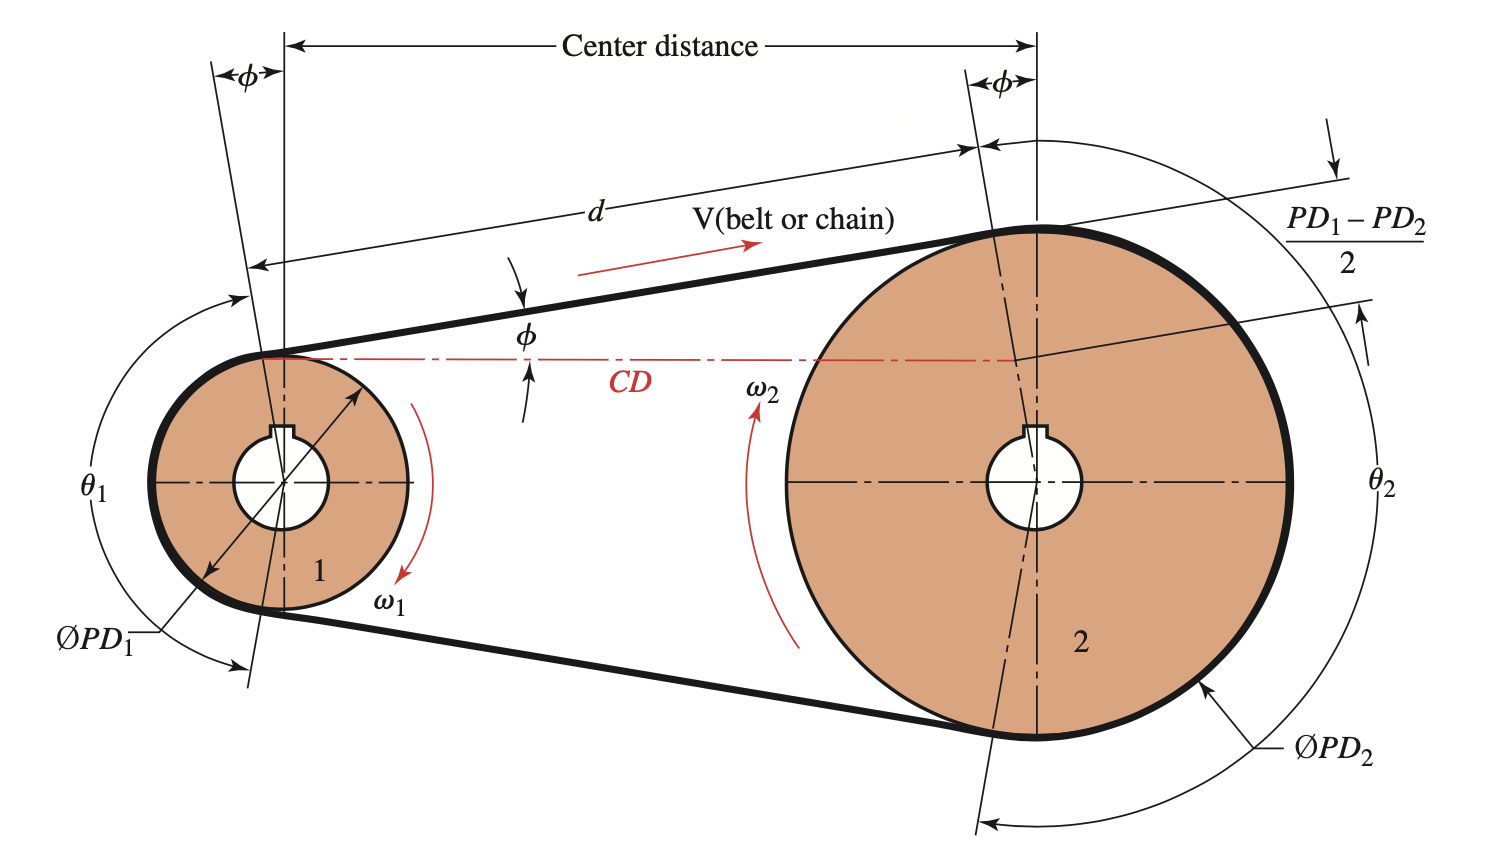
\includegraphics[scale=0.6]{Belts/configuration.png}\\
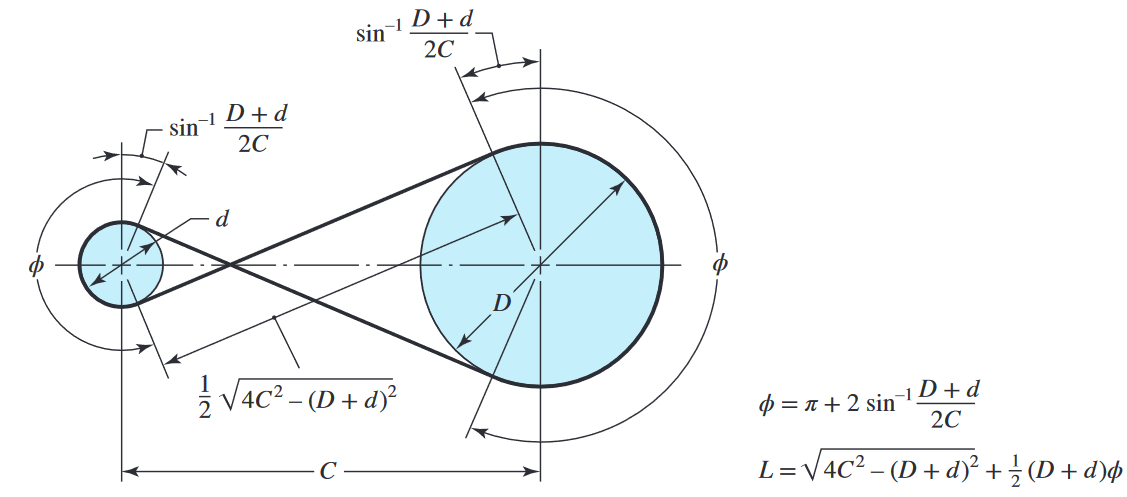
\includegraphics[scale=0.45]{Gears/Twist.png}\\
\subsection{General Nomenclature}
$PD=D=$ pitch diameter (in)\\
$\omega=n=$ angular speed of sprocket/sheave (rpm)\\
$VR=$ velocity ratio\\
$v_b=$ belt speed\\
$CD=$ center distance (in)\\
$\text{\o}=$ random angle that helps solve for the wrap angle ($^\circ$)\\
$\theta=$ angle of wrap ($^\circ$)\\
$s=$ arc length (length of belt/chain wrap on sprocket)\\
$d=$ distance (or span) (belt/chain length that is tangent to sprockets)\\
$L_p=$ belt/chain total length\\
$H_{in}=$ input power (hp)\\
$P_{des}=$ power (hp)\\
$P_{rated}=$ rated power (hp)\\
$SF=$ service factor

\subsection{Flat Belts}
\subsubsection{Nomenclature}
    $F_1=$ taut-side tension\\
    $F_2=$ slack-side tension\\
    $F_c=$ centrifugal tension\\
    $F_i=$ initial tension\\
    $f=$ maximum coefficient of friction\\
    $T=$ transmitted torque\\
    $w= $ weight per foot ($\mathrm{lb/ft}$)\\
    $V= $ belt speed ($\mathrm{ft/min}$)\\
    $H=$ transmitted power ($\mathrm{hp}$)\\
    $b=$ belt width ($\mathrm{in}$)\\
    $t=$ belt thickness ($\mathrm{in}$)\\
    $\gamma$ = specific weight ($\mathrm{lb/in^3}$)\\
    $(F_1)_a= $largest allowable tension\\
    $F_a= $ allowable tension/unit width\\
    $C_P=$ pulley correction factor (tab. 17-4)\\
    $C_V=$ velocity correction factor (p. 889)\\
    $H_\text{nom}=$ nominal (rated) power\\
    $H_a=$ design power\\
    $K_s=$ service factor\\
    $n_d= $ design safety factor\\
    $n_f=$ factor of safety\\
    $n=$ angular velocity ($\mathrm{rpm}$)
\subsubsection{Formulae}
    $\Delta F=(F_1)_a-F_2=\frac{2T}{d}$\\
    $F_1-F_2=\frac{2T}{d}$\\
    $F_1=F_c+\frac{2F_ie^{f\phi}}{e^{f\phi}+1}$\\
    $F_2=F_c+\frac{2F_i}{e^{f\phi}+1}$\\
    $\frac{F_1-F_c}{F_2-F_c}=e^{f\phi}$\\
    $F_c=\frac{w}{32.17\,\mathrm{ft/s^2}}\brround{\frac{V}{60\,\mathrm{s/min}}}^2$\\
    $F_i=\frac{F_1+F_2}{2}-F_c=\frac{T}{d}\frac{e^{f\phi}+1}{e^{f\phi}-1}$\\
    $H=\frac{(F_1-F_2)V}{33,000\,\mathrm{(\frac{ft\,lb}{min})/hp}}$\\
    $w=12\,\mathrm{in/ft}\,\gamma bt$\\
    $(F_1)_a=bF_aC_PC_V$\\
    $H_d=H_\text{nom}K_sn_d$\\
    $H_a=H_\text{nom}K_sn_d$\\
    $n_\text{fs}=\frac{H_a}{H_\text{nom}K_s}$\\
    $T=63025\frac{H_\text{nom}K_sn_d}{n}=63025\frac{H_d}{n}$\\
    $f'=\frac{1}{\phi}\ln\brround{\frac{(F_1)_a-F_c}{F_2-F_c}}$\\
    $\text{dip}=\frac{C^2w}{96\,\mathrm{in/ft}F_i}$\\
    $F_1=(F_1)_a$ at operation limit\\
        require $f'<f$
\subsubsection{Tables for Constants}
    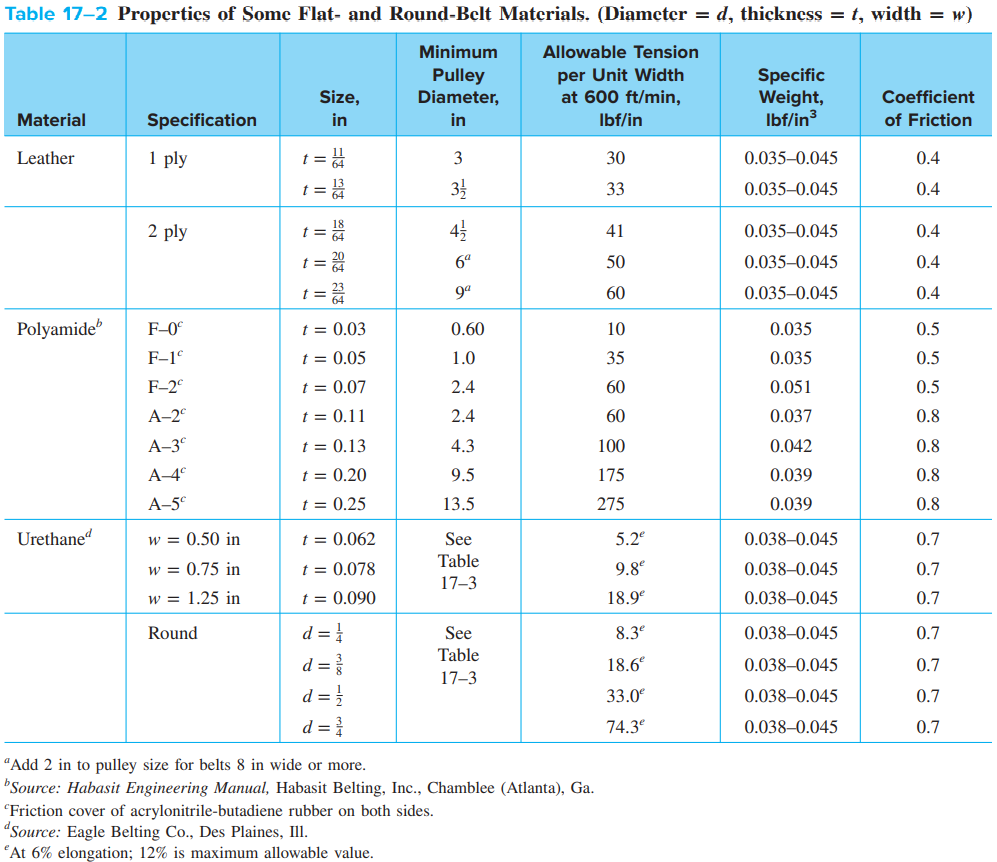
\includegraphics[scale = 0.5]{Belts/Table 17-2.png}\\
    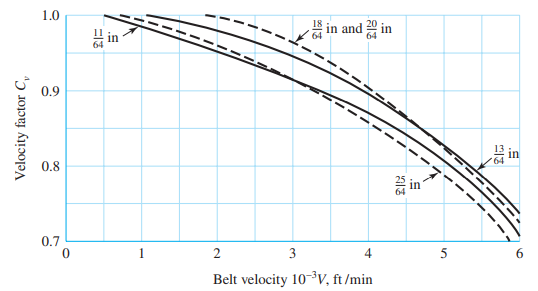
\includegraphics[scale = 0.9]{Belts/Fig17-9.png}\\
    $C_v = 1$ for polyamide and urethane belts\\
    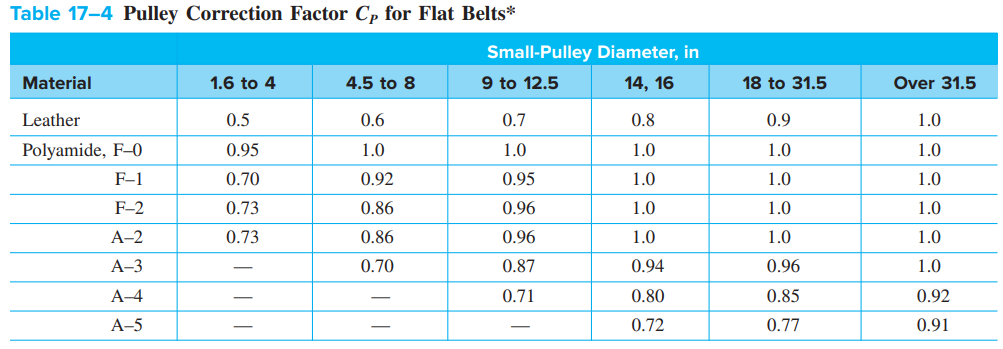
\includegraphics[scale = 0.5]{Belts/Table 17-4.png}
\subsection{V-Belt Drives}
\subsubsection{Anatomy}
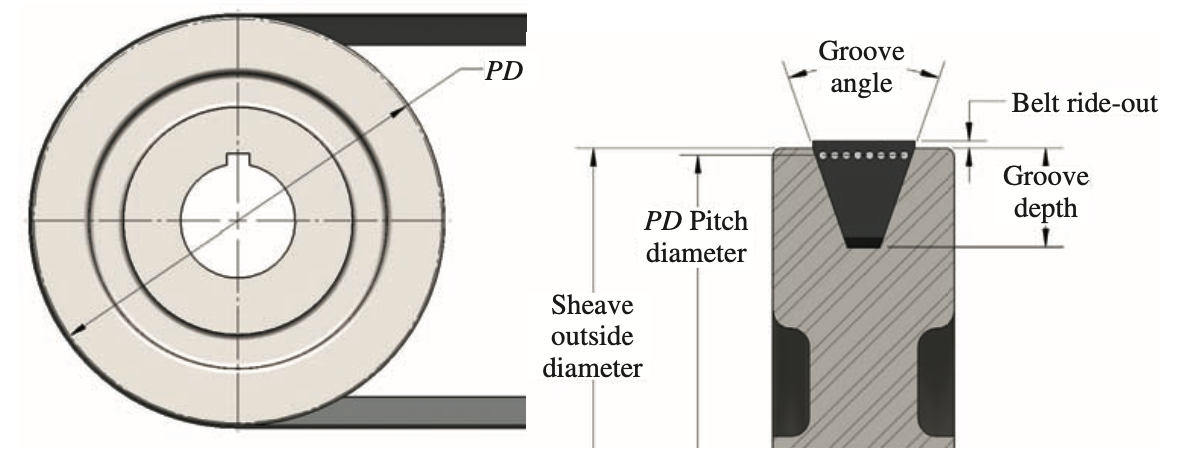
\includegraphics[scale=0.6]{Belts/v-belt_pd.png}
\subsubsection{Design Selection}
\begin{enumerate}
    \item Compute the design power
    \begin{enumerate}
        \item Find the service factor based from this table:\\
        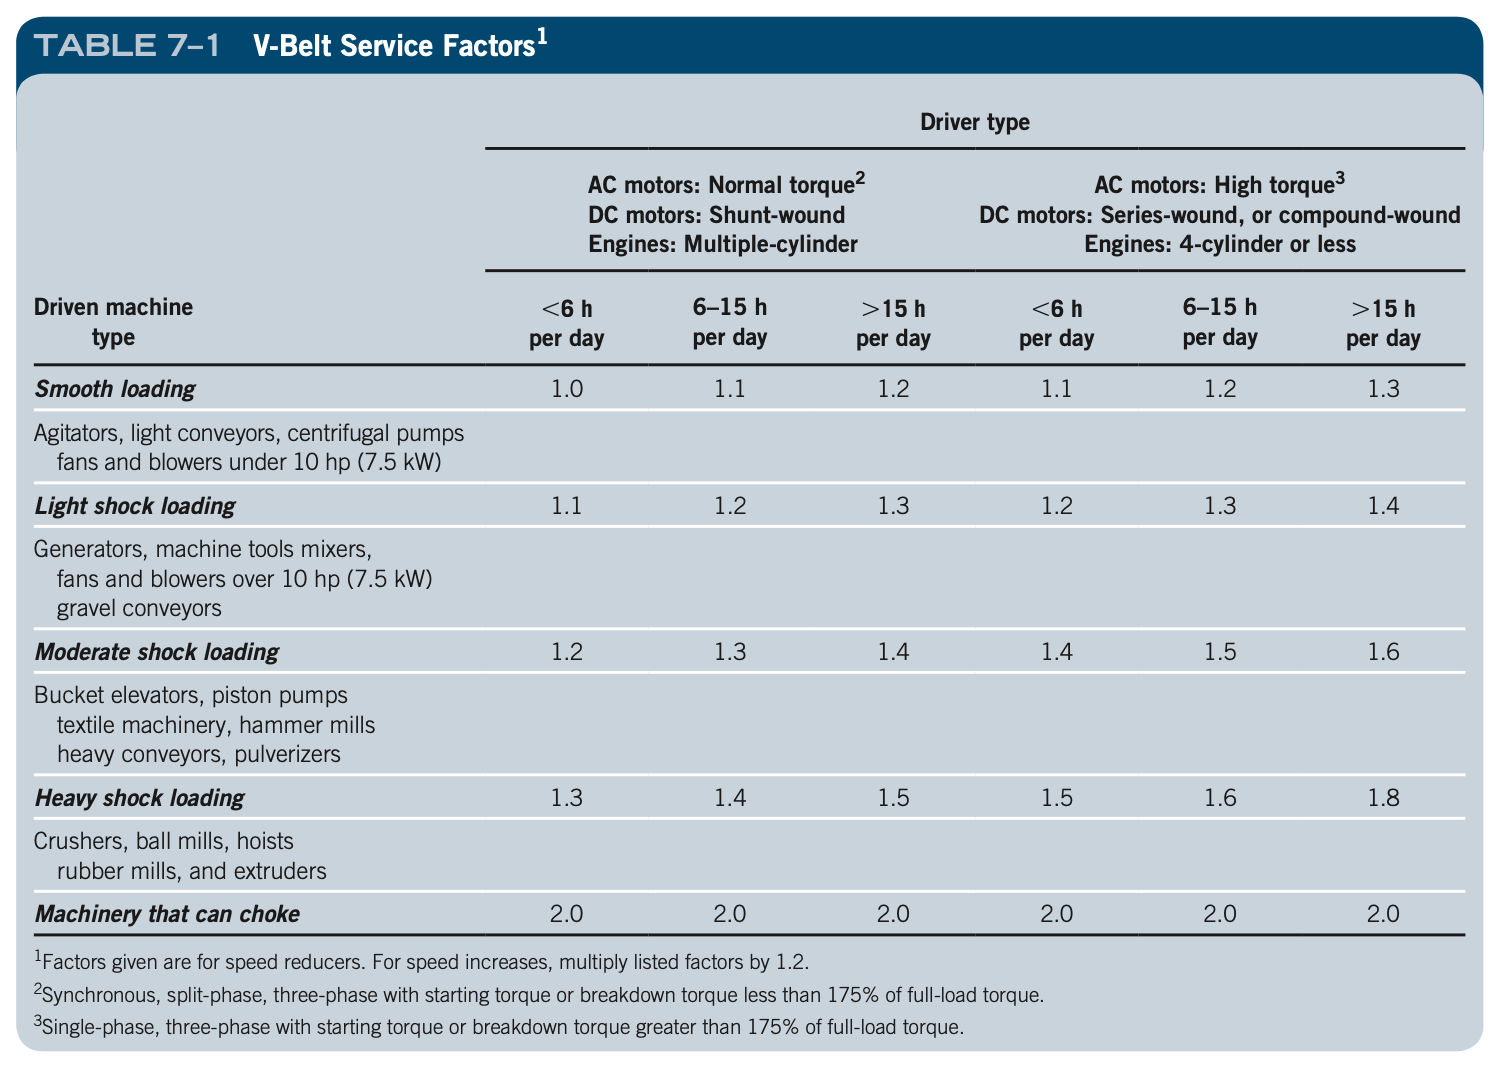
\includegraphics[scale=0.55]{Belts/7-1.png}
        \item Compute design power using:
        \begin{align*}
            P_{des}=H_{in}\cdot SF
        \end{align*}
    \end{enumerate}
    \item Select the belt section\\
    If at the boundary between two different types of belts, be
    conservative and choose the larger one\\
    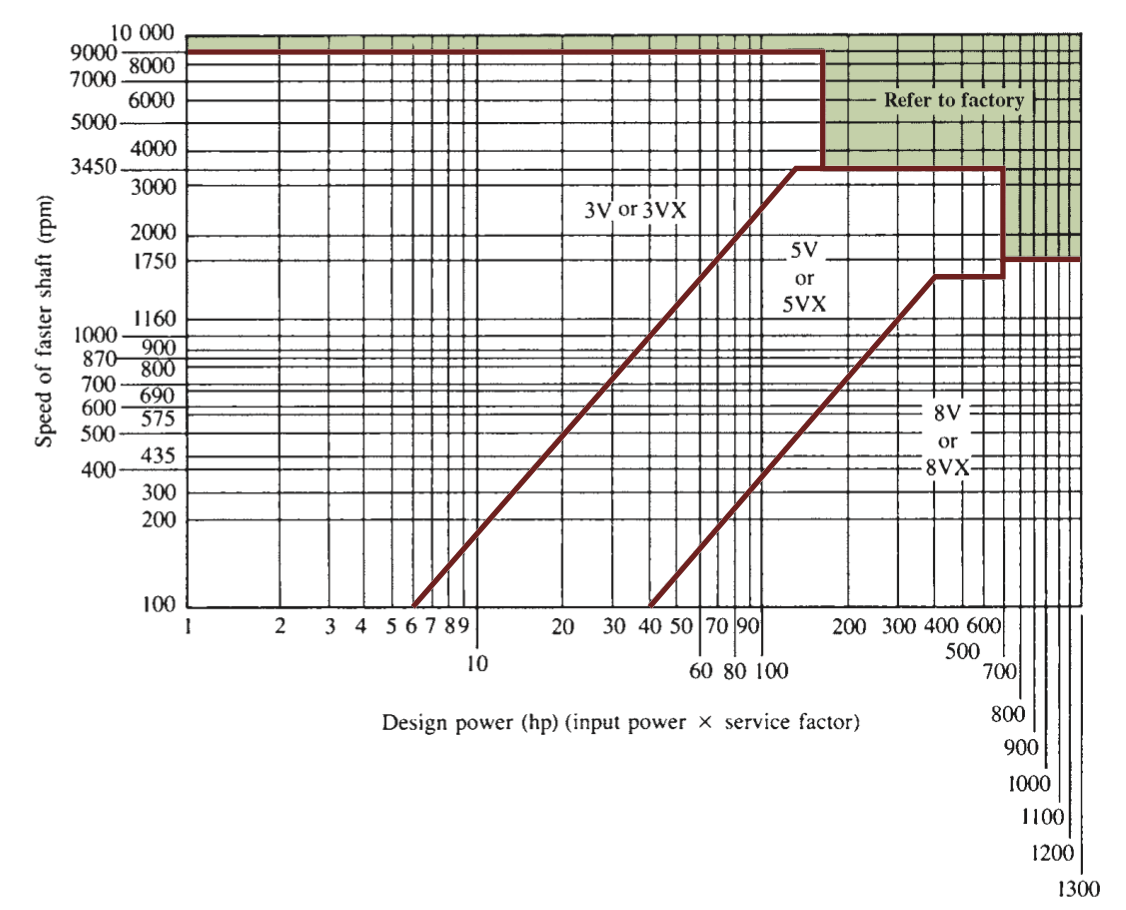
\includegraphics[scale=0.8]{Belts/7-13.png}
    \item Compute the nominal speed ratio
    \begin{align*}
        VR=\frac{n_1}{n_2} \text{ where } n_1 > n_2
    \end{align*}
    \item Select the driving sheave size to produce a belt speed of 4000 ft/min (this is a standard speed we use since belt speed should not surpass 5000 ft/min, with a hard max at 6500 ft/min)
    \begin{align*}
        v_b=\frac{D_1n_1}{2}\cdot(12 \text{ in/ft})(1 \text{ rev/}(2\pi\text{ rad}))
    \end{align*}
    \item Select the standard sizes for the input and output sheaves\\
    \begin{enumerate}
        \item Select the closest standard size to the input sheave
        For 3V belts:\\
        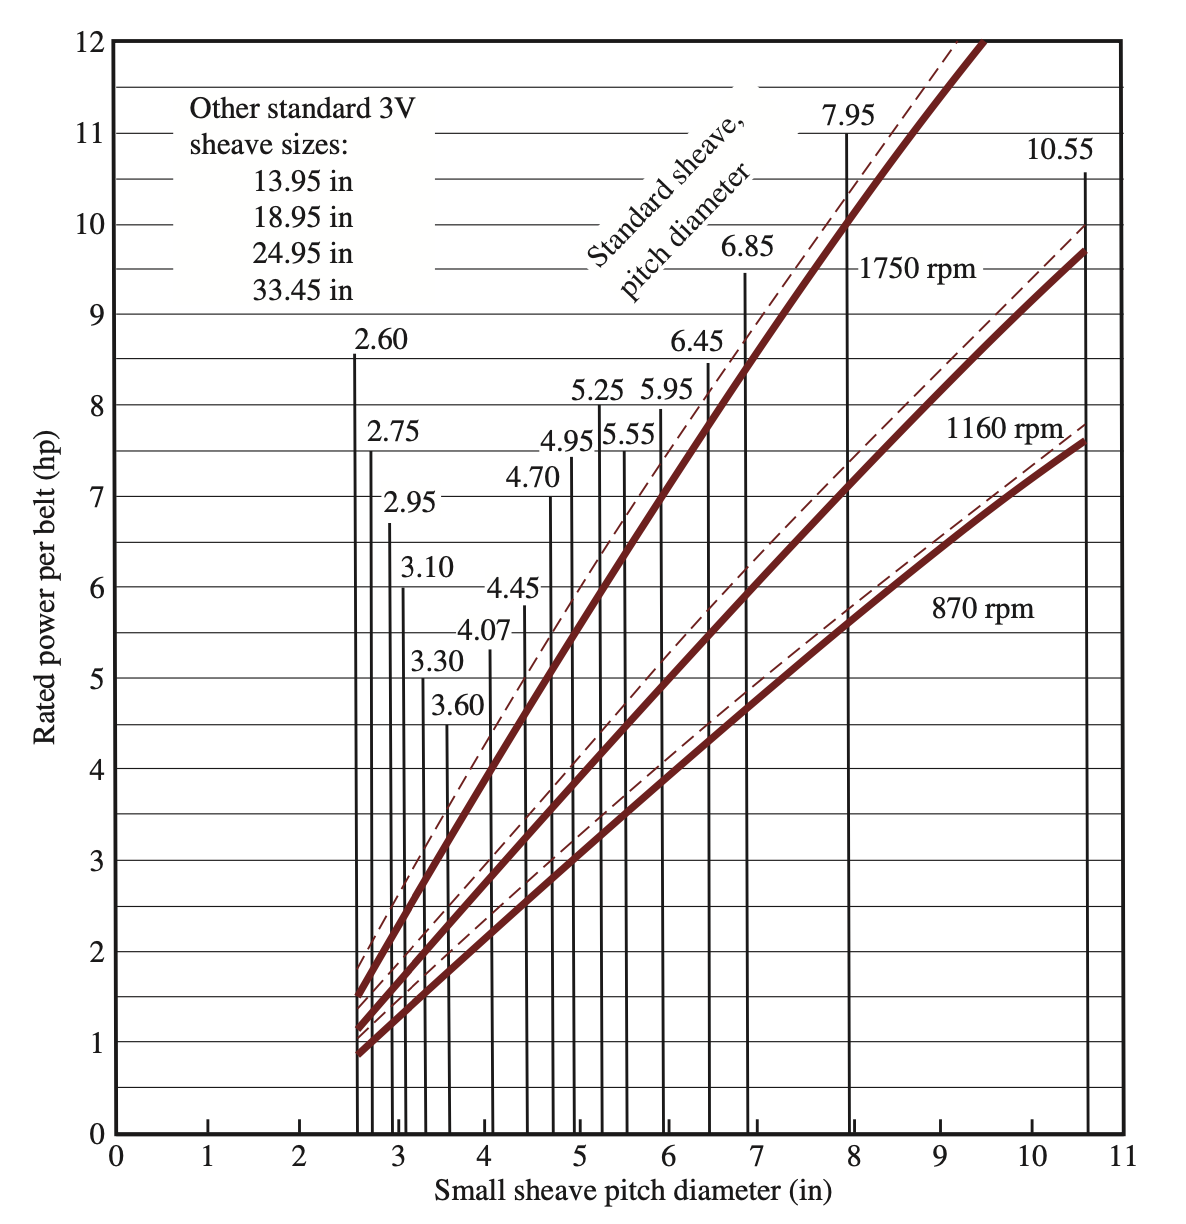
\includegraphics[scale=0.3]{Belts/standard_3V.png}\\
        For 5V belts:\\
        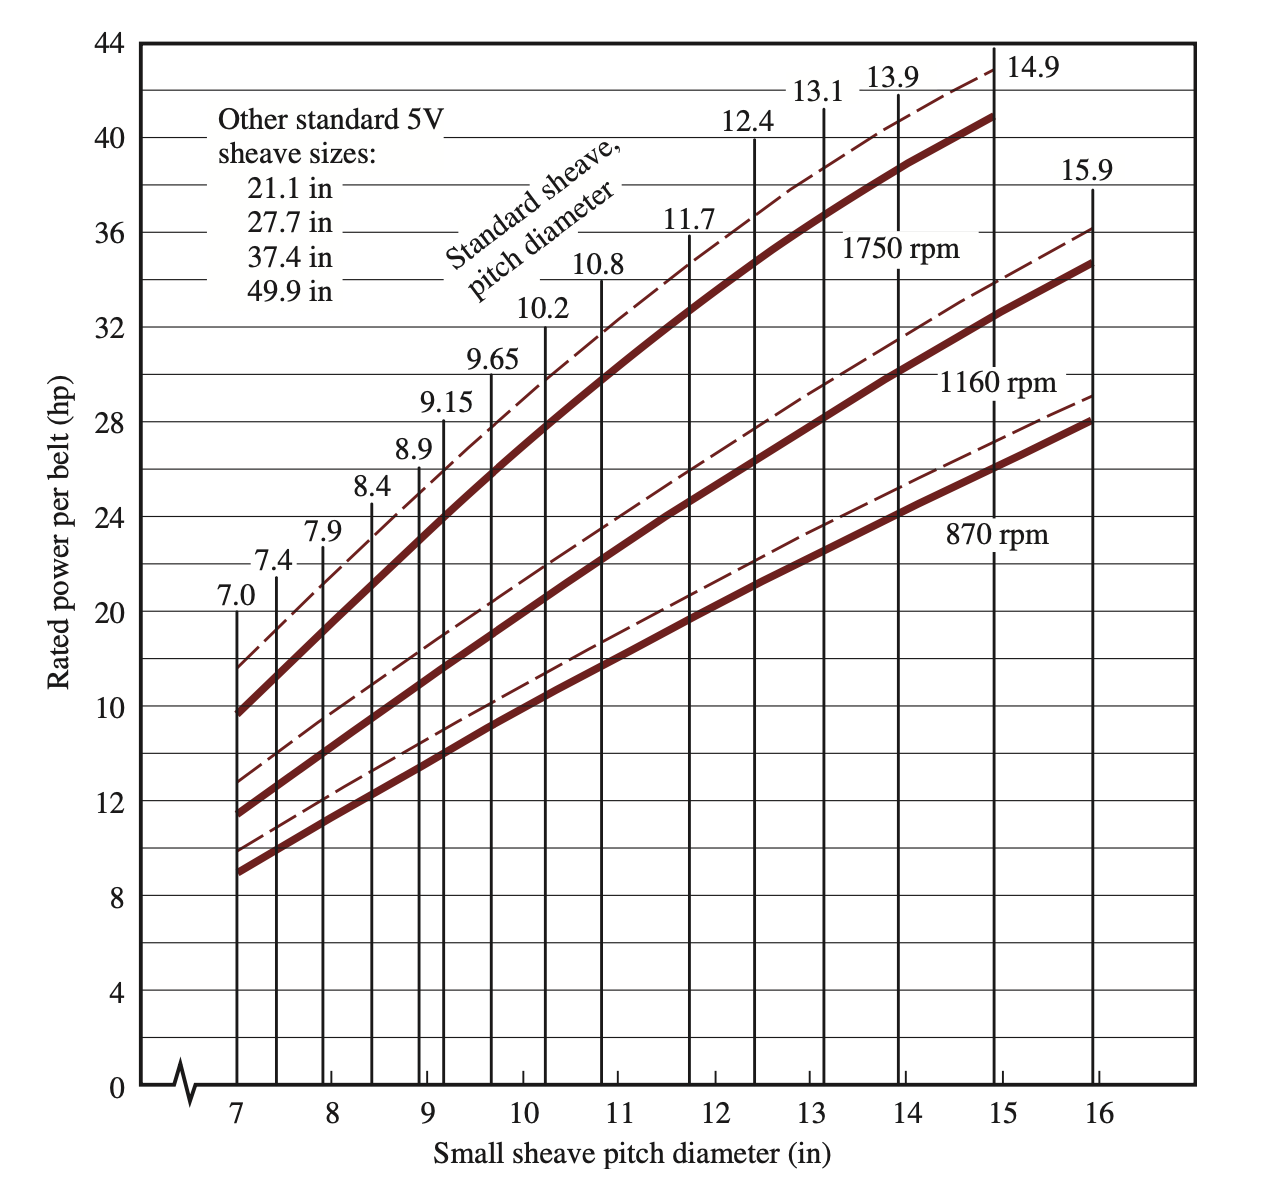
\includegraphics[scale=0.6]{Belts/standard_5V.png}\\
        For 8V belts:\\
        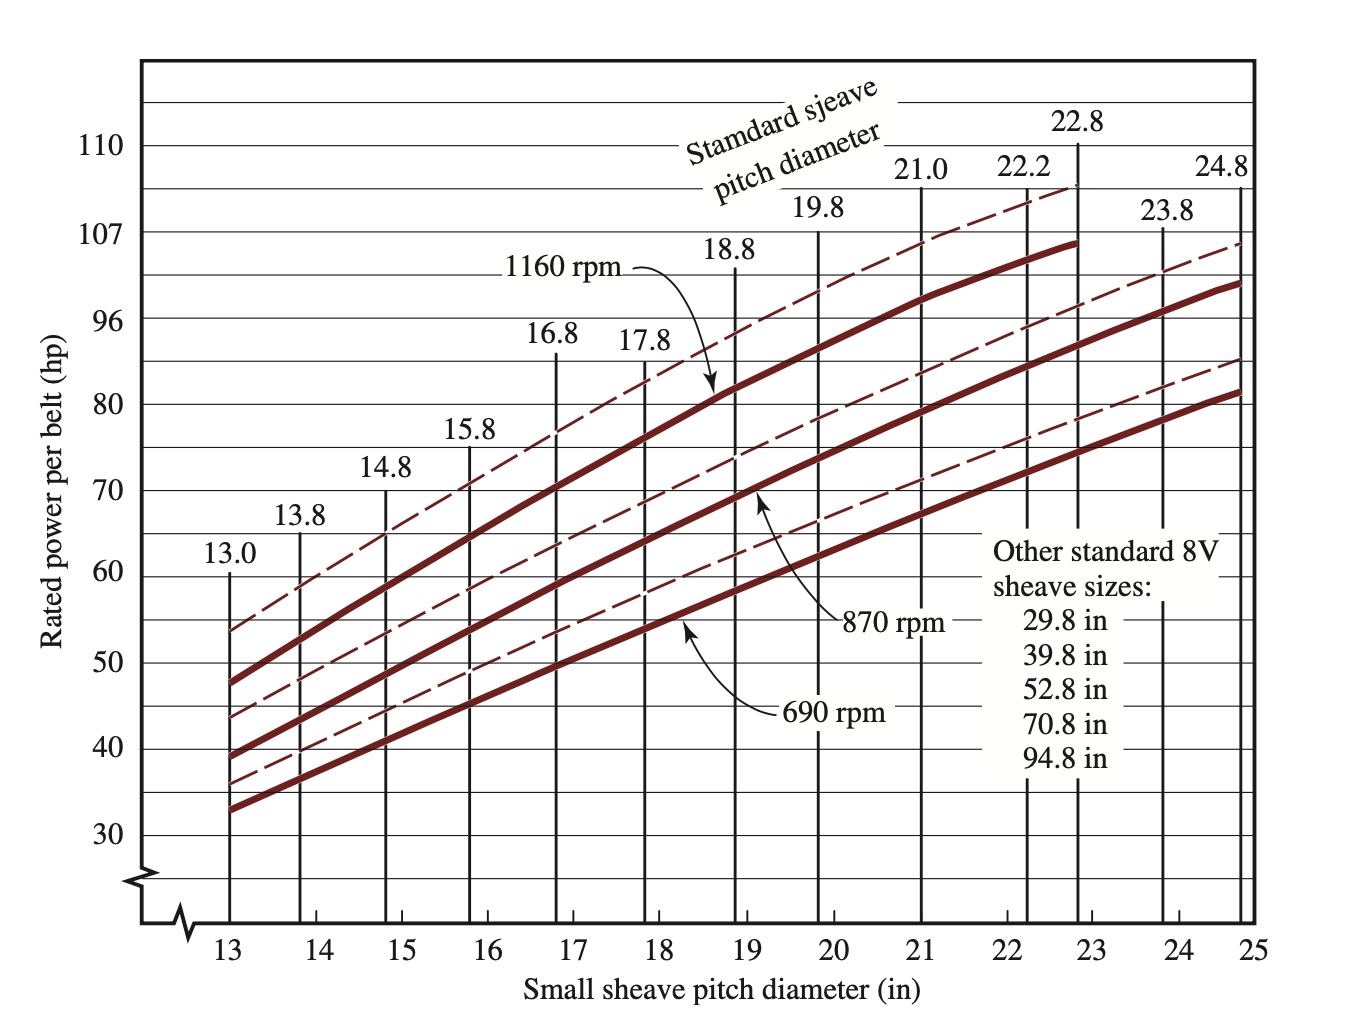
\includegraphics[scale=0.6]{Belts/standard_8V.png}
        \item Find the output sheave size using $D_2=D_1\cdot VR$ where $D_2 > D_1$
        \item Find the closest standard size to the output sheave using the same figures as above
    \end{enumerate}
    \item Compute the actual speed ratio and belt speed
    \begin{align*}
        VR=\frac{D_2}{D_1}\\
        v_b=\frac{D_1n_1}{2}\cdot(12 \text{ in/ft})(1 \text{ rev/}(2\pi\text{ rad}))
    \end{align*}
    \item Determine the rated power per belt
    \begin{enumerate}
        \item Use the above figures to find the rated power per belt
        \item If the actual speed ratio is higher than 1, use the following table to find the power added:\\
        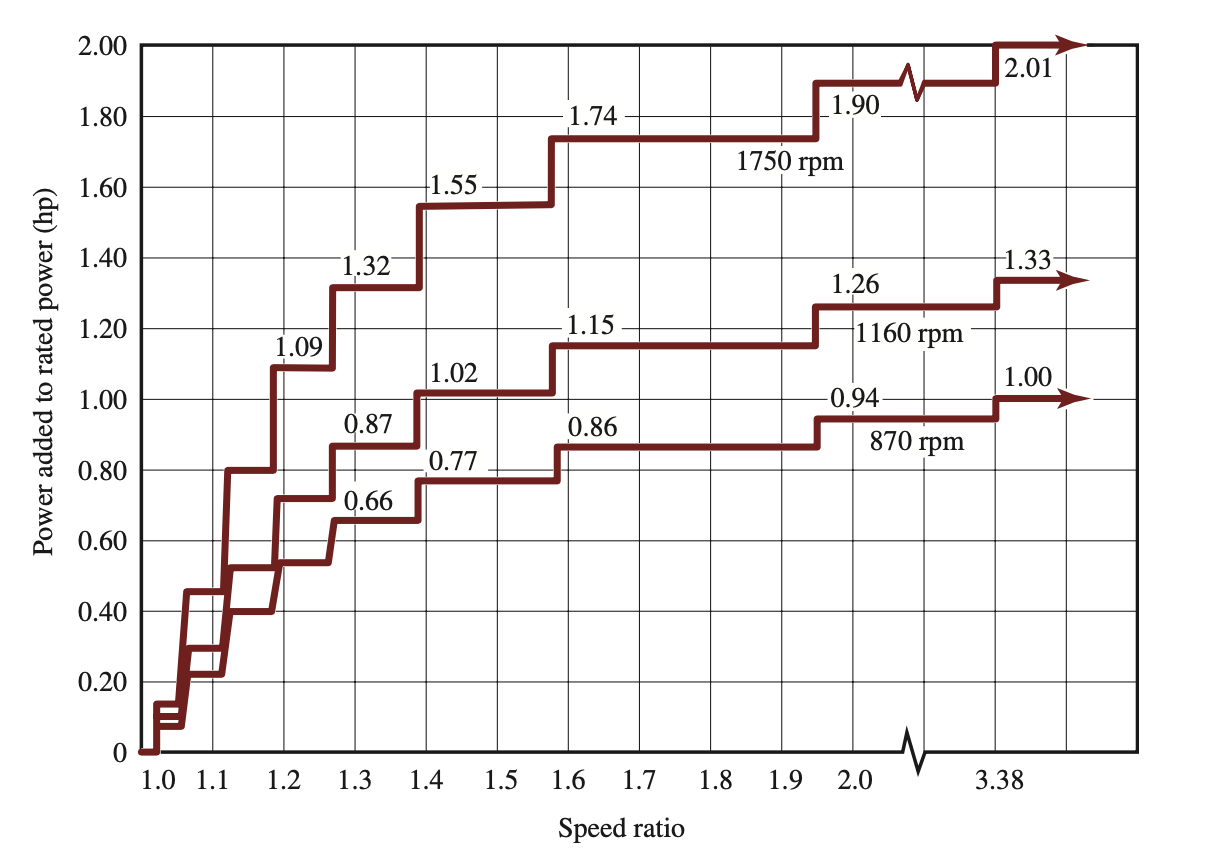
\includegraphics[scale=0.3]{Belts/7-17.png}
        \item The total rated power per belt ($P_{rated}$) is the sum of both
    \end{enumerate}
    \item Specify a trial center distance, CD, that is within the following range:
    \begin{align*}
        D_2 < CD < 3(D_2+D_1)
    \end{align*}
    \item Compute the required belt length
    \begin{align*}
        L_p=2CD+1.57(D_2+D_1)+\frac{(D_2-D_1)^2}{4C}
    \end{align*}
    \item Select the closest standard belt length value from the following table:\\
    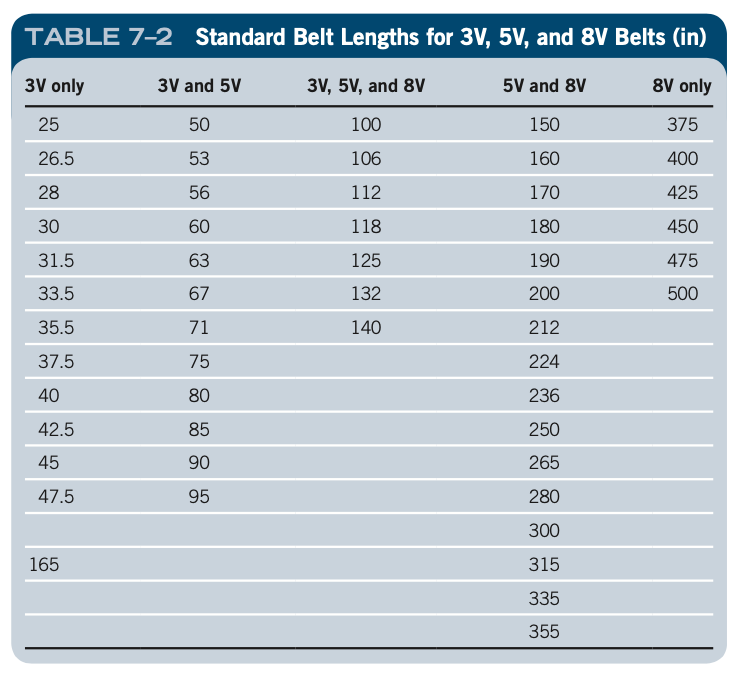
\includegraphics[scale=0.7]{Belts/standard_lengths.png}
    \item Using the standard belt length, compute the actual CD. First compute B (a random constant) cause it'll help simplify the CD expression
    \begin{align*}
        B=4L_p-6.28(D_2+D_1)\\
        CD=\frac{B+\sqrt{B^2-32(D_2-D_1)^2}}{16}
    \end{align*}
    \item Compute the angle of wrap of small sheave
    \begin{align*}
        \theta_1=180^\circ-2\sin^{-1}\brround{\frac{D_2-D_1}{2CD}}
    \end{align*}
Probably won't be asked to compute the angle of wrap for the big sheave, but just in case, here is the formula:
    \begin{align*}
        \theta_2=180^\circ+2\sin^{-1}\brround{\frac{D_2-D_1}{2CD}}\\
    \end{align*}
    \item Determine the angle of wrap correction factor $C_{\theta}$\\
    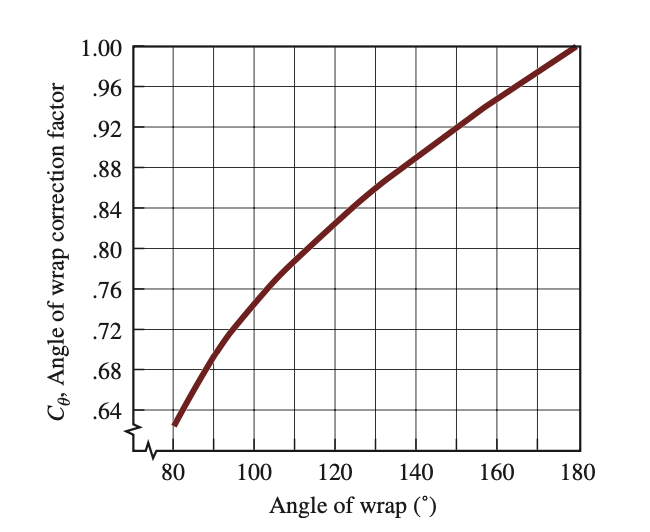
\includegraphics[scale=1]{Belts/7-18.png}
    \item Determine the belt length correction factor $C_{L_p}$\\
    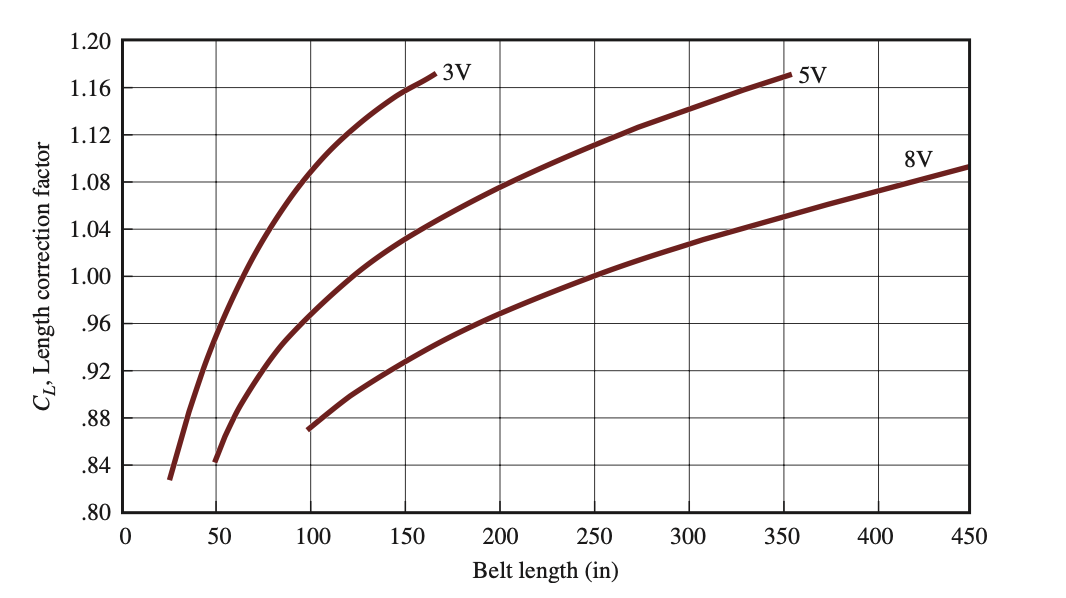
\includegraphics[scale=0.8]{Belts/7-19.png}
    \item Determine the required number of belts\\
    \begin{enumerate}
        \item Calculate the corrected power rating $=C_{\theta}C_{L_p}P$
        \item Calculate the minimum number of belts required
        \begin{align*}
            \text{min number of belts}=\frac{\text{design power}}{\text{corrected power rating}}
        \end{align*}
        \item Round up to the nearest integer
    \end{enumerate}
\end{enumerate}
And that's it! You're doing great!!!

\subsection{Synchronous Belt Drives}
\subsubsection{Anatomy}
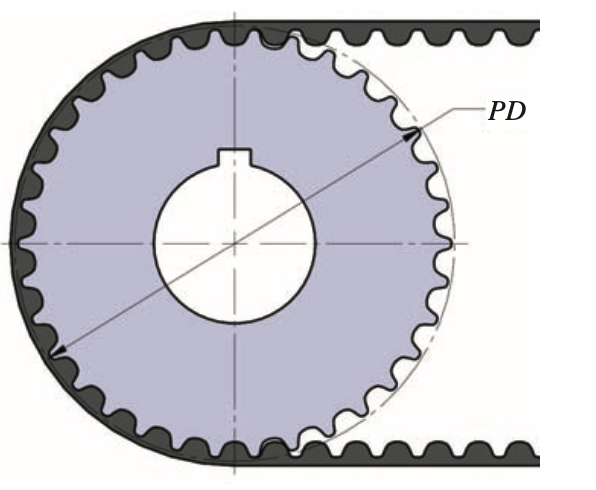
\includegraphics[scale=0.6]{Belts/sync-belt_pd.png}
\subsubsection{Design Selection}
\begin{enumerate}
    \item Compute the design power\\
    \begin{enumerate}
        \item Find the service factor from this table\\
        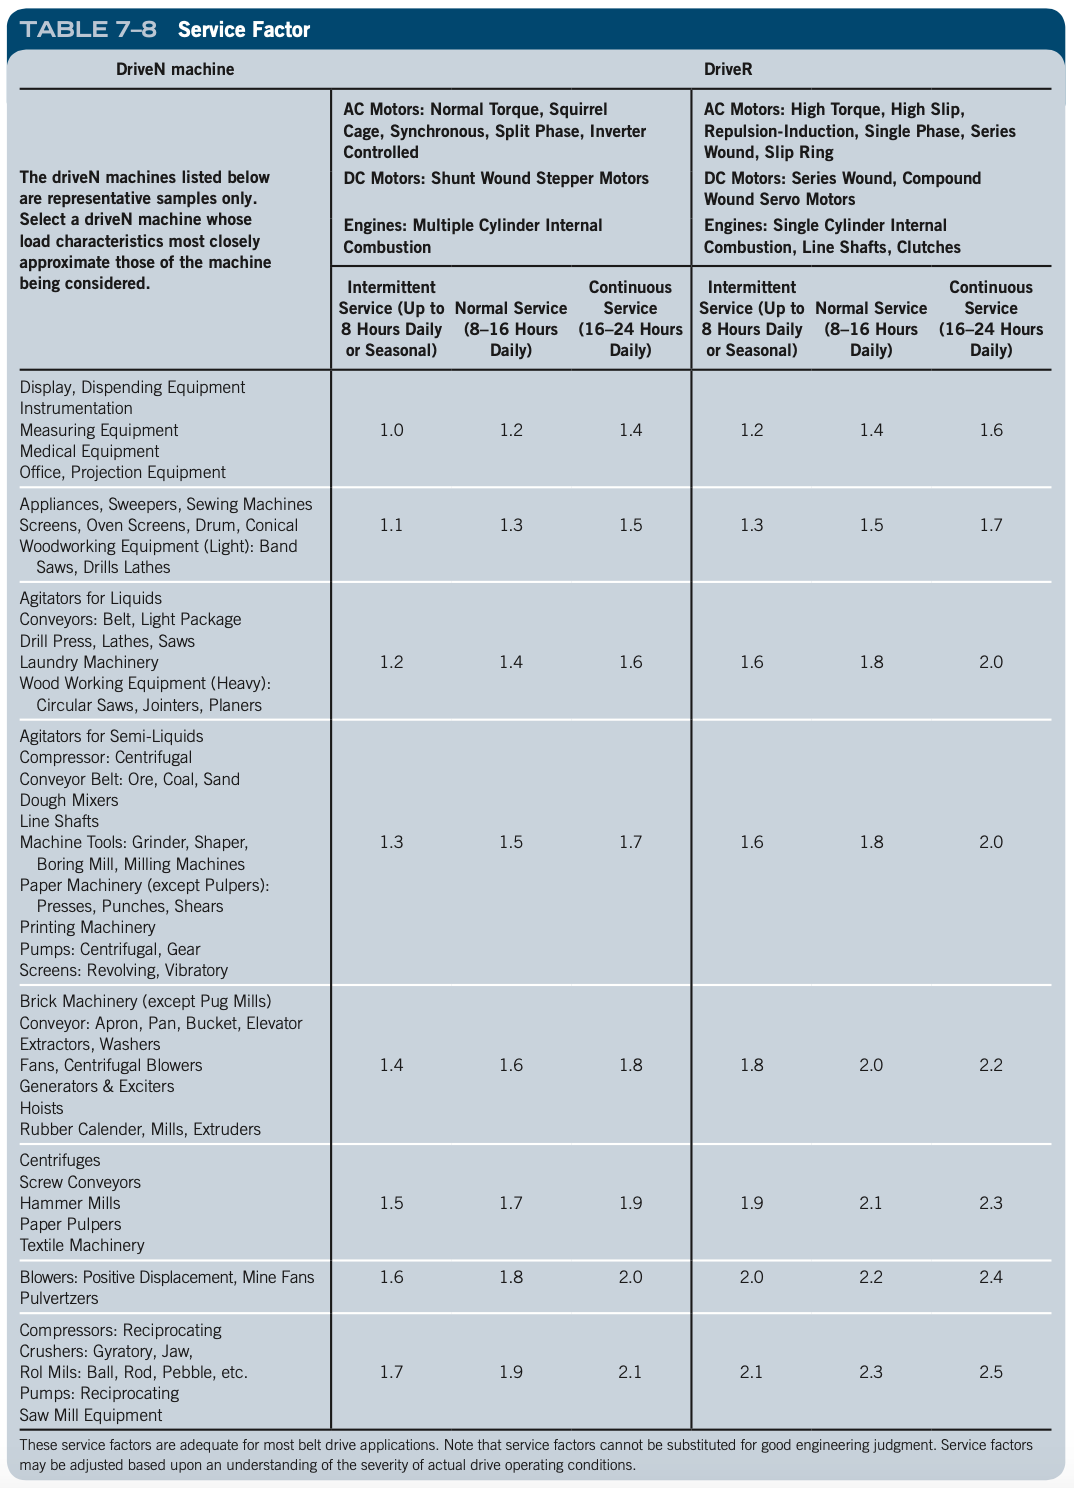
\includegraphics[scale=0.8]{Belts/7-8.png}
        \item $P_{des}=P_{rated}\cdot SF$
    \end{enumerate}
    \item Find the required pitch for the belt using this figure:\\
    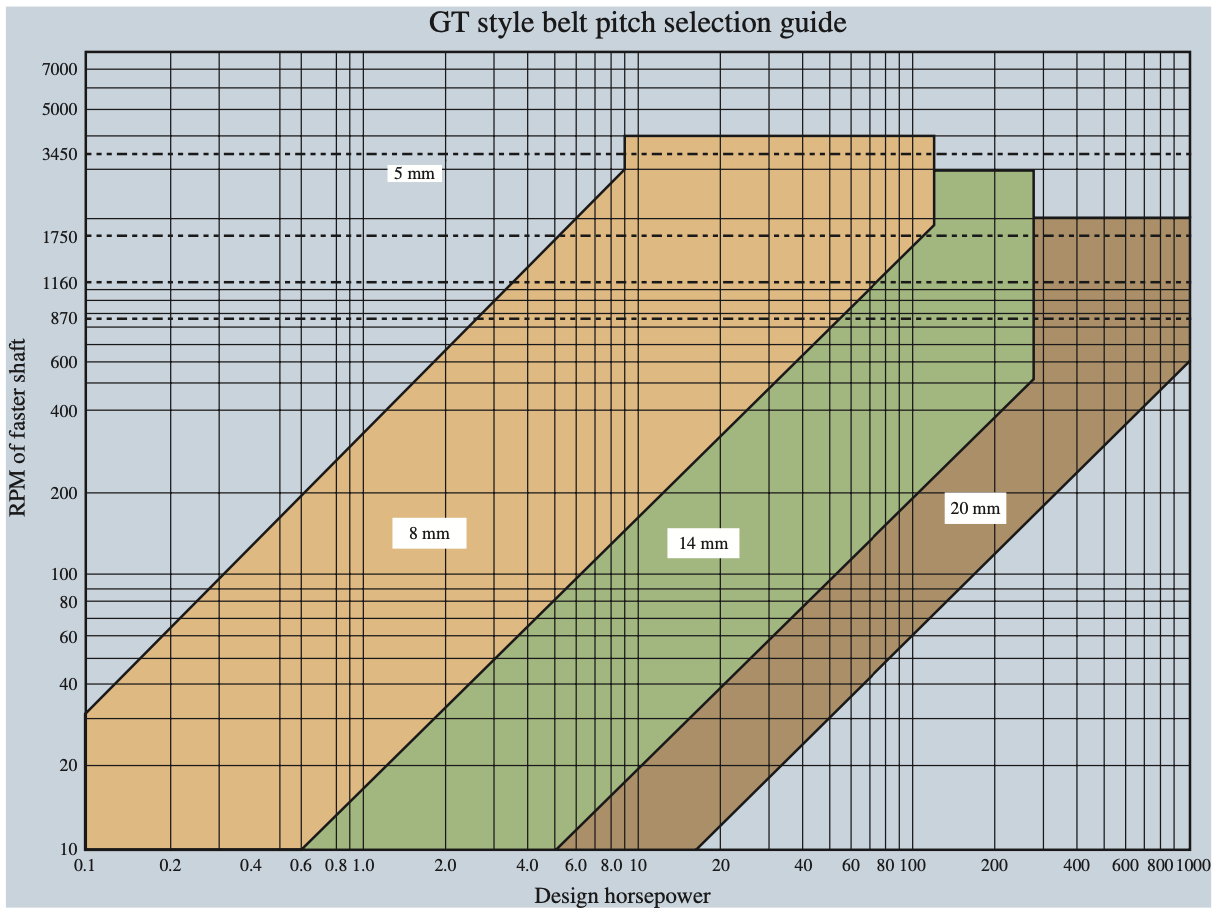
\includegraphics[scale=0.7]{Belts/required_pitch.png}\\
    (You're probably going to get an 8mm pitch because that is all this textbook has data for...)
    \item Compute the velocity ratio using $VR=\frac{n_{\text{driving}}}{n_{\text{driven}}}$
    \item Select candidate combinations of driver and driven sprockets based on the VR.\\
    You should have multiple possible combinations. List them all out, and then we will eliminate some in the next step.\\
    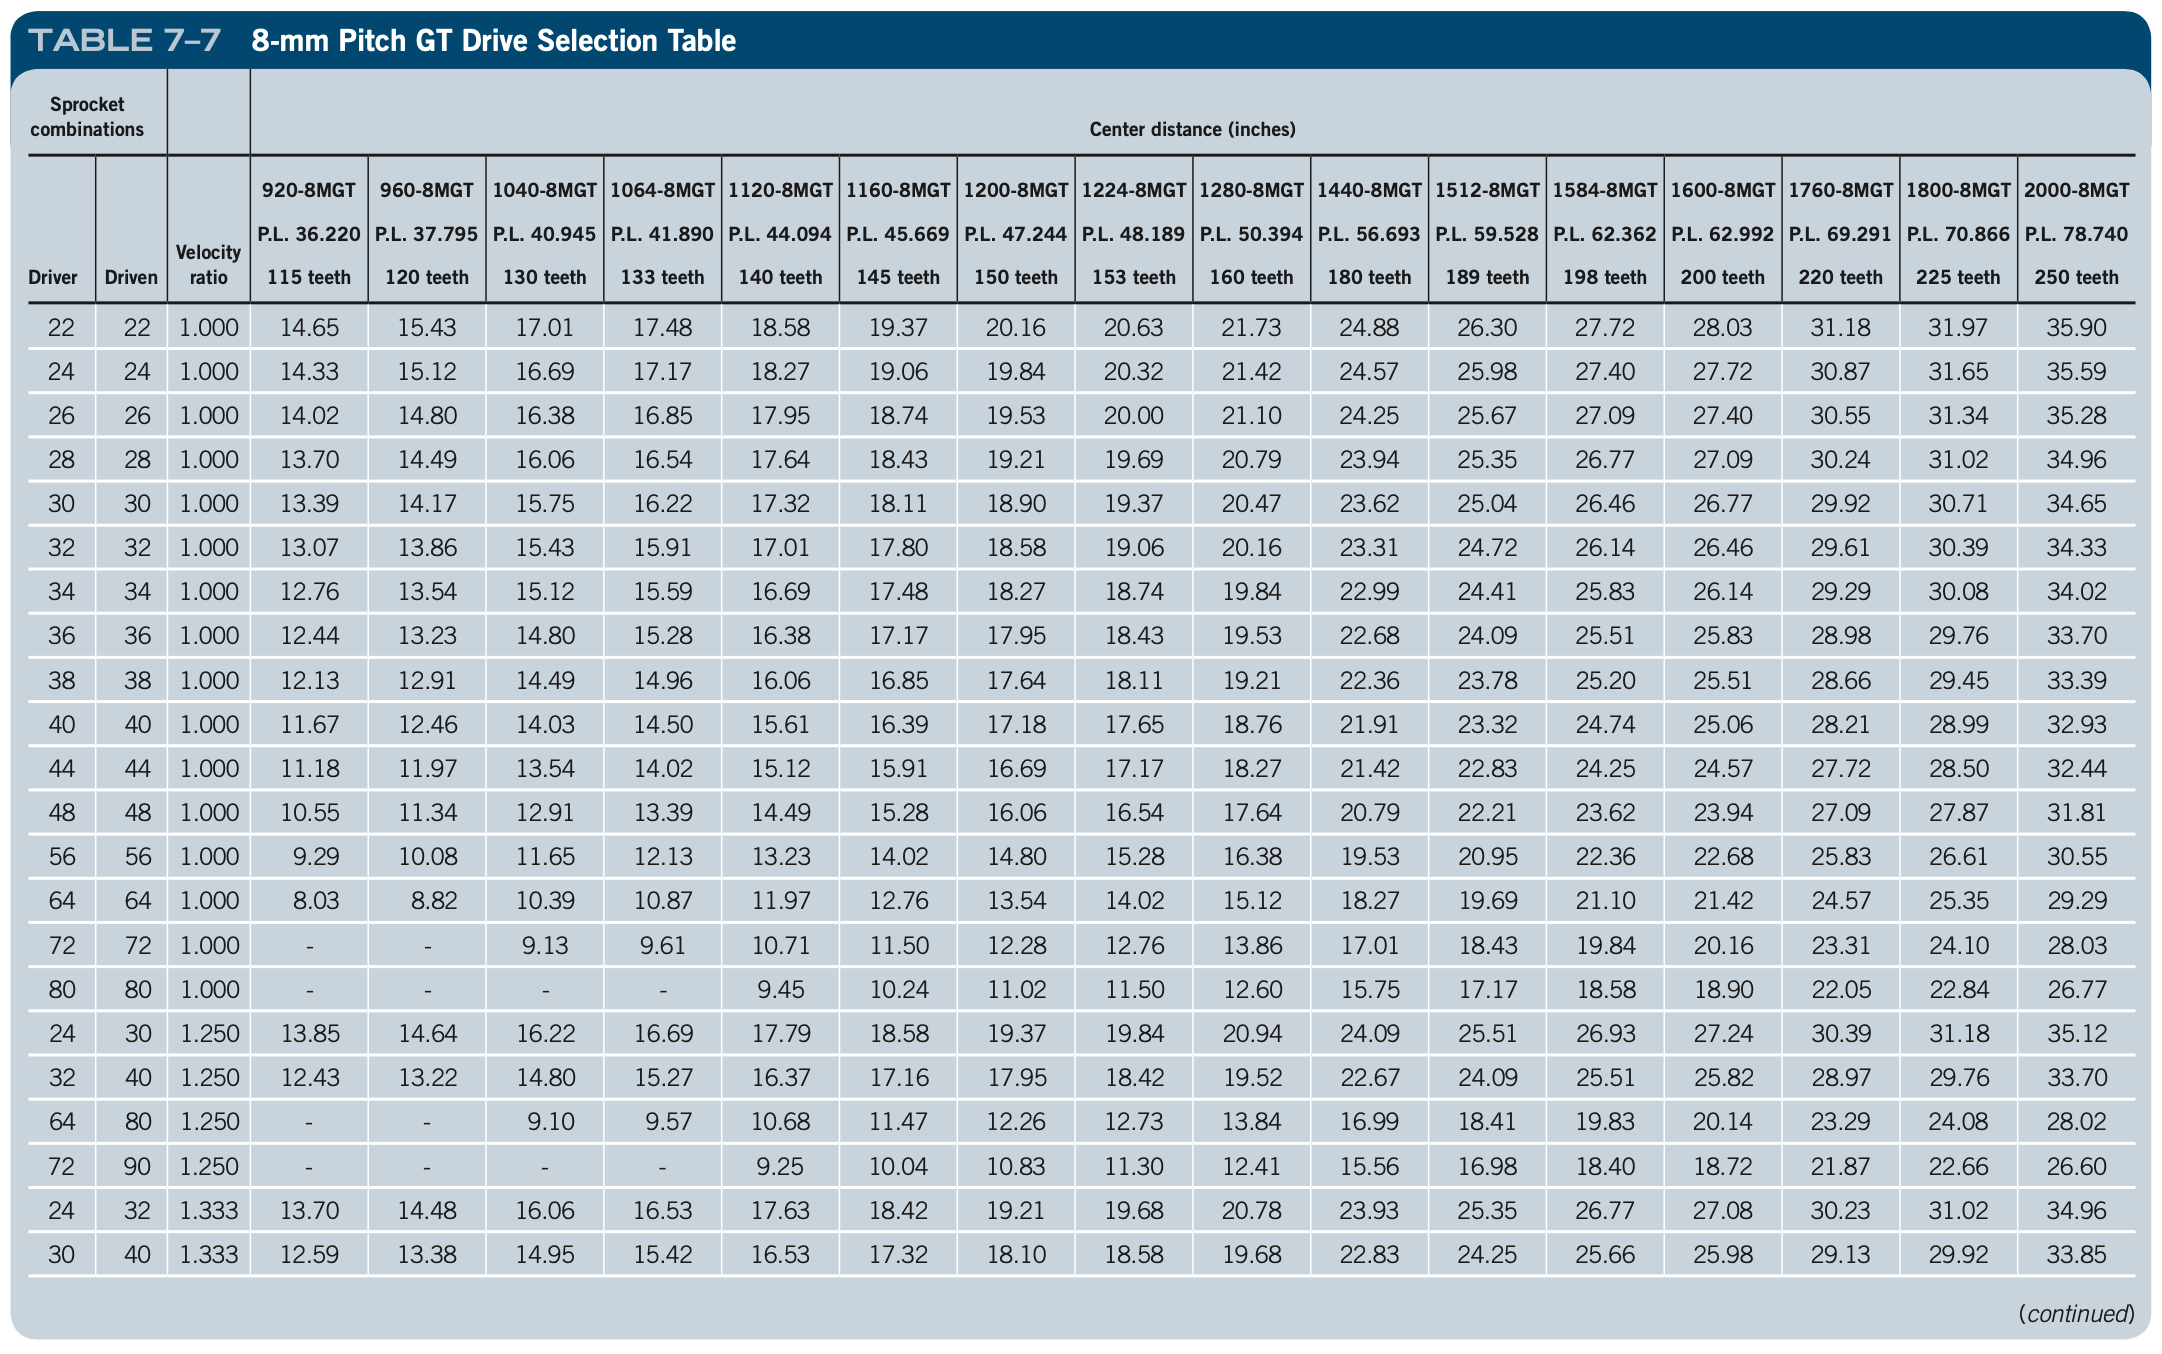
\includegraphics[scale=0.4]{Belts/7-7_part1.png}\\
    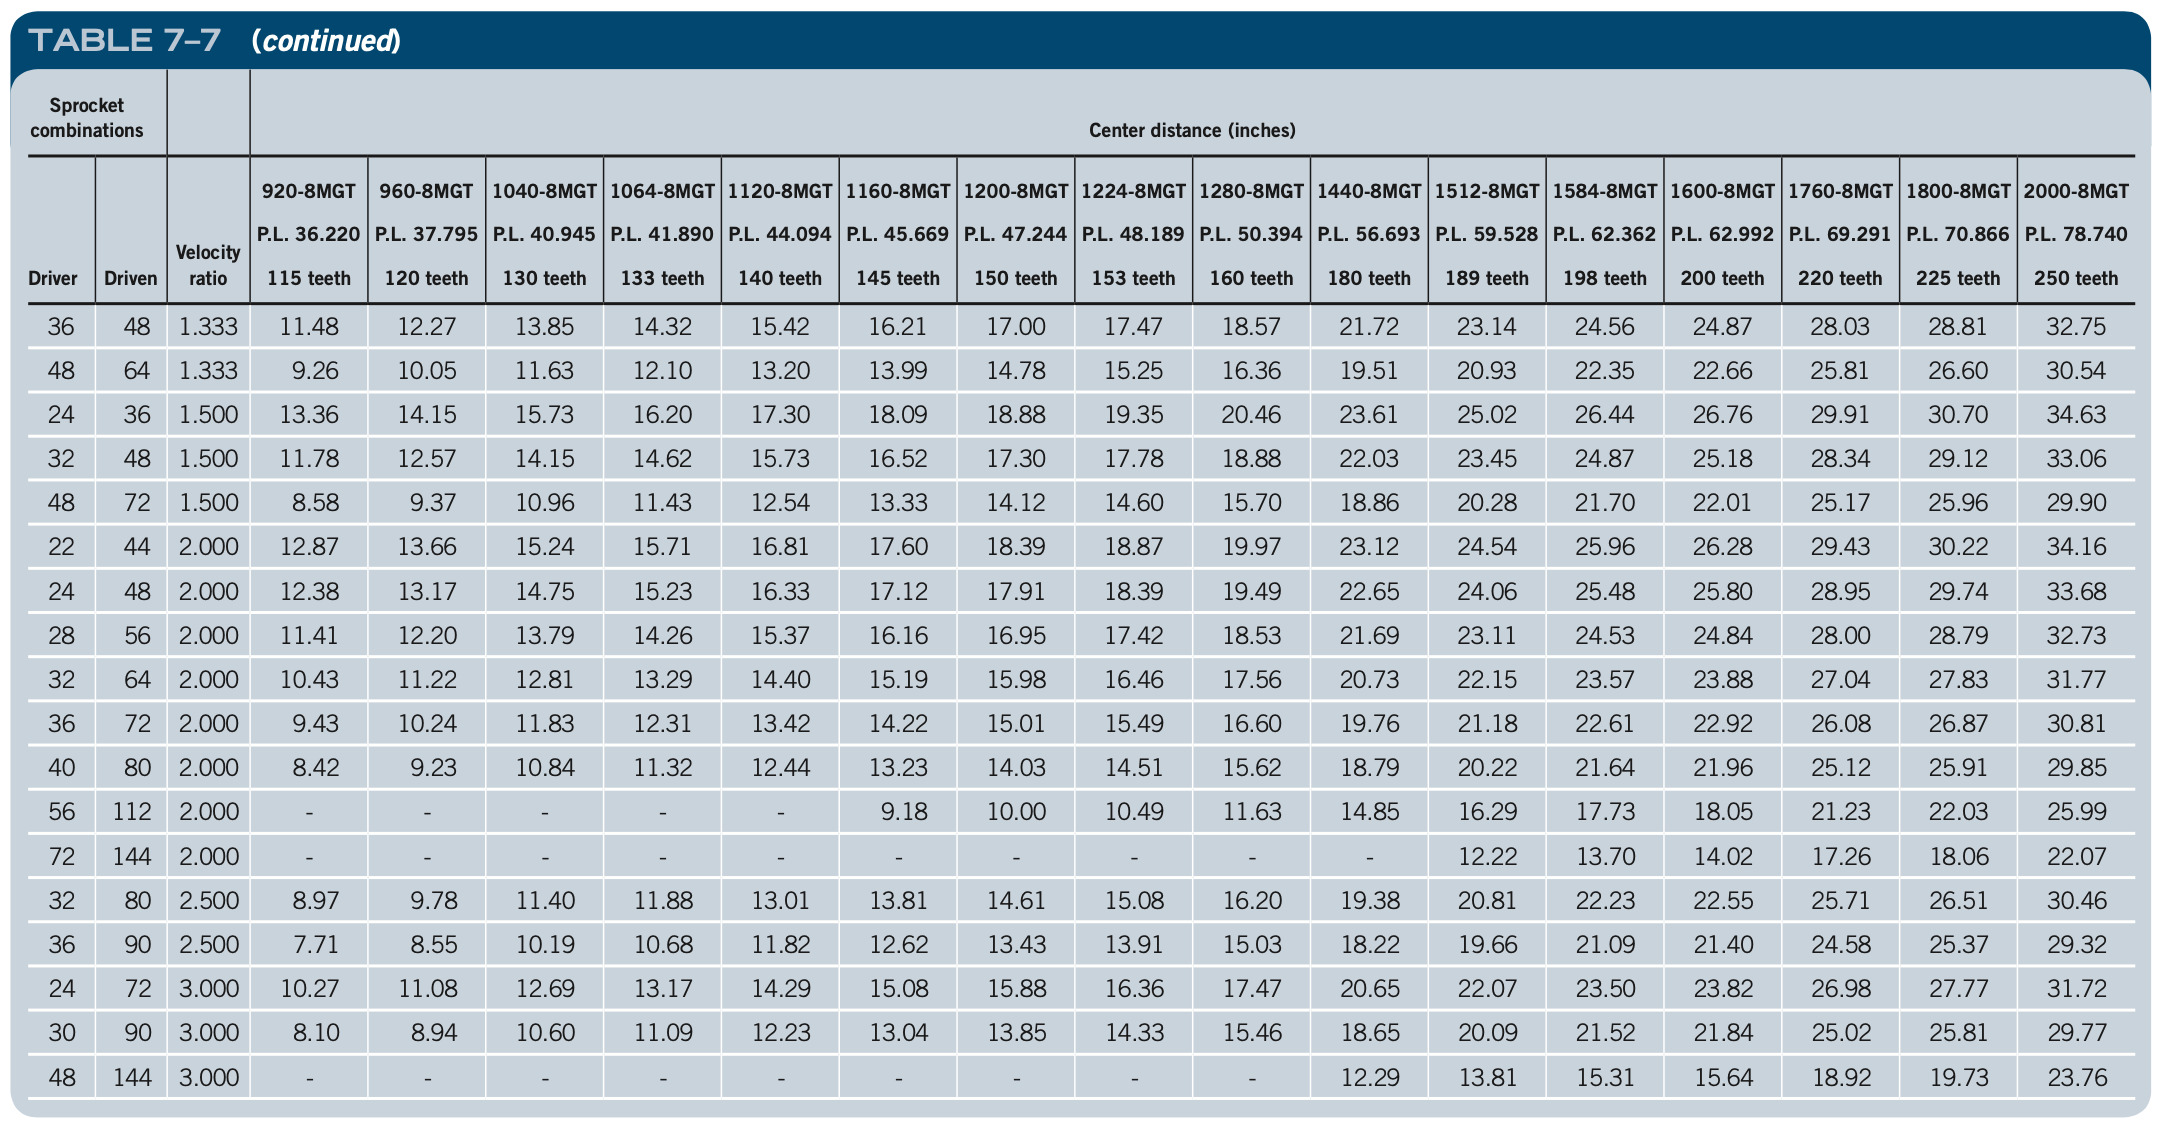
\includegraphics[scale=0.4]{Belts/7-7_part2.png}
    \item Eliminate sprockets that are not acceptable due to shaft requirements and space limitations
    \begin{enumerate}
        \item If the motor shaft size is given, you must ensure the driving sprocket's max bore size is bigger than the motor shaft (I think the bore is the hole in the middle of the sprocket)\\
        First you're going to want to find the brushing size for the candidate driving sprockets\\
        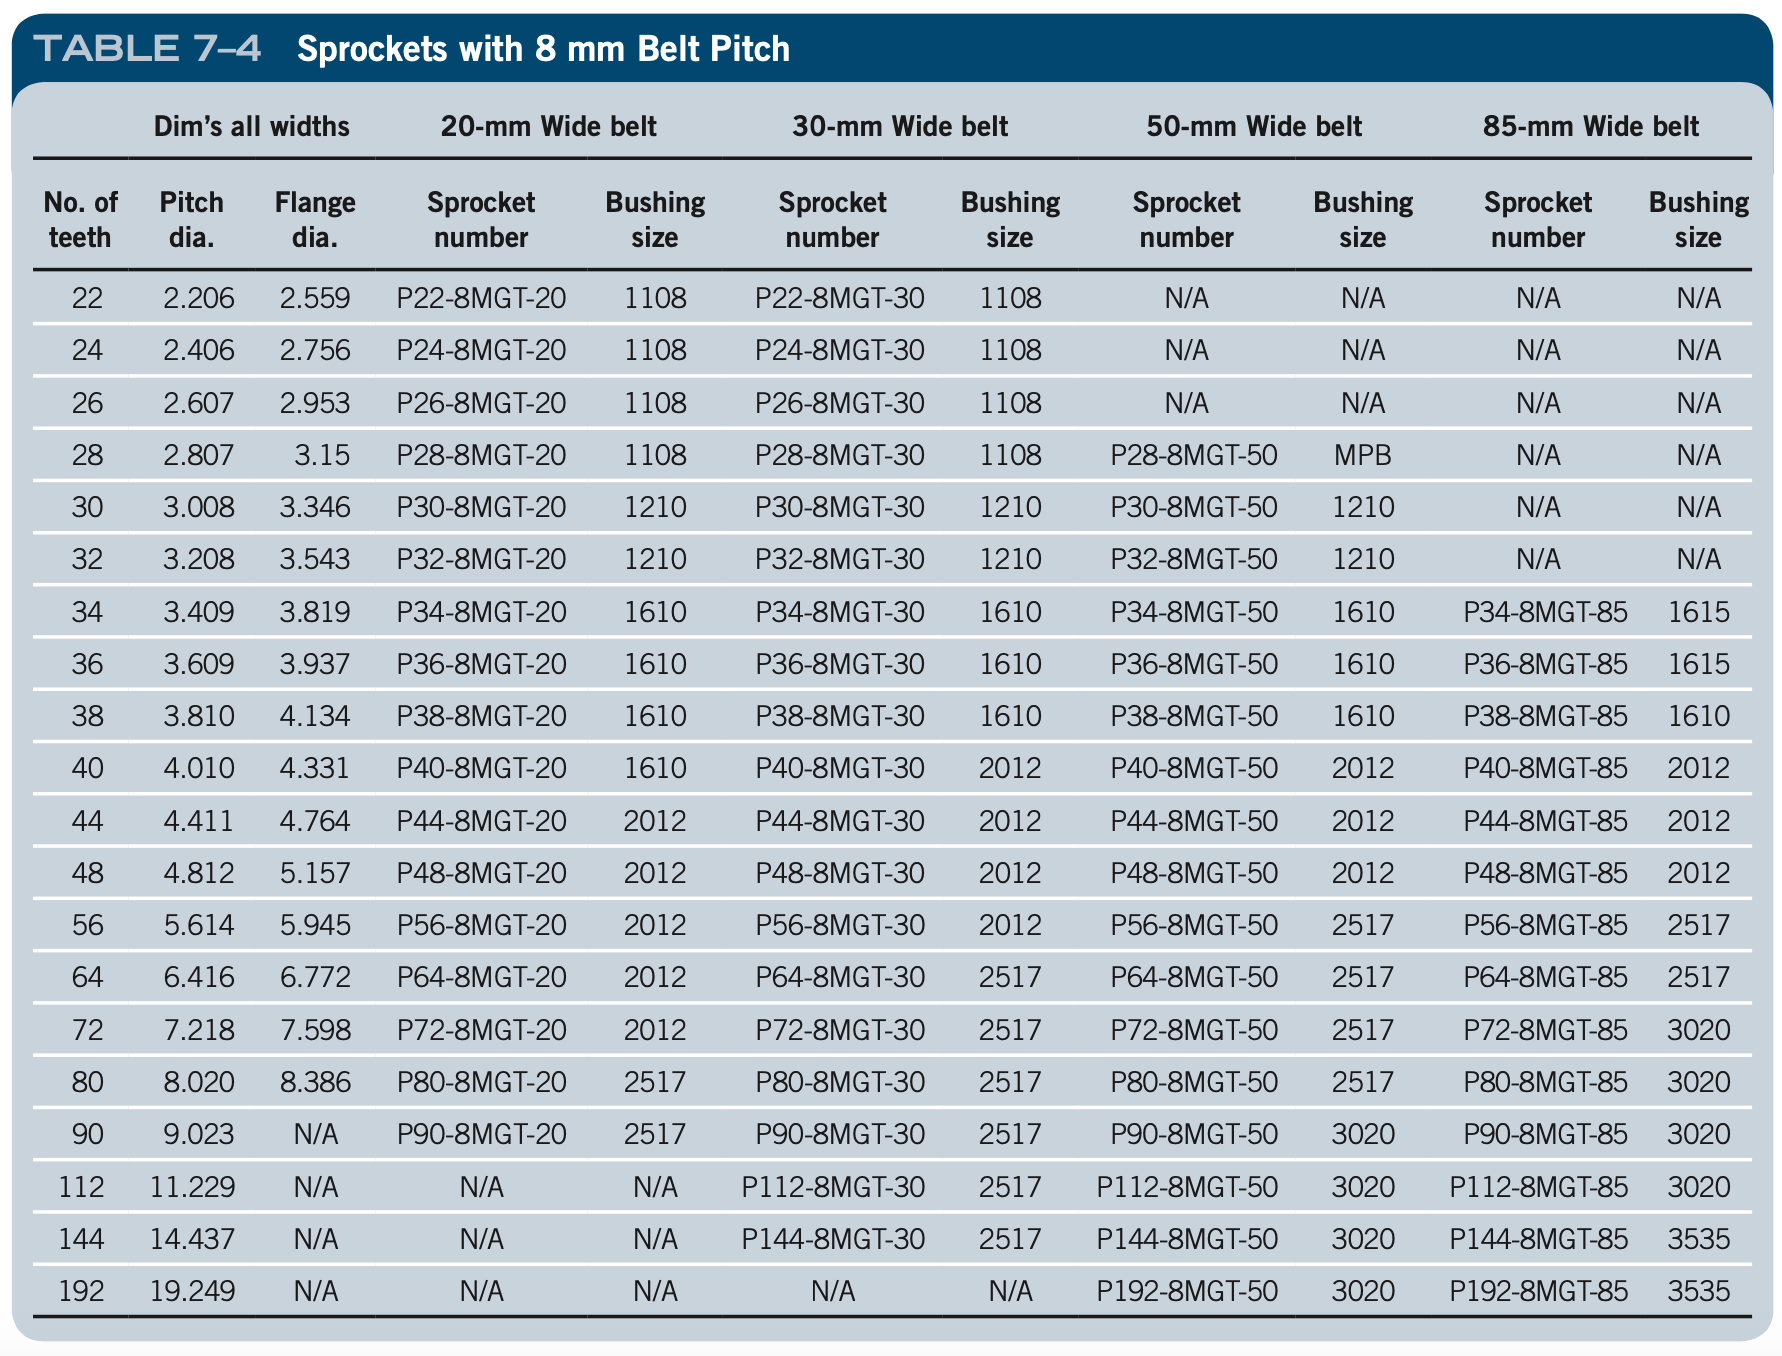
\includegraphics[scale=0.45]{Belts/7-4.png}\\
        Then find the associated bore sizes from here:\\
        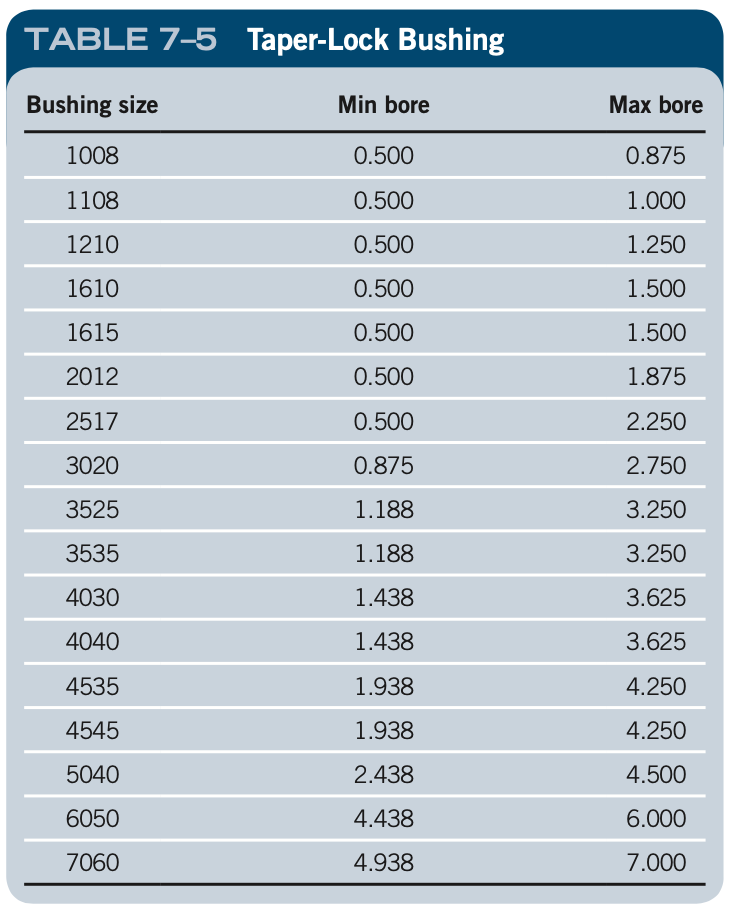
\includegraphics[scale=0.6]{Belts/7-5.png}\\
        Eliminate the sprocket combinations that have a driving sprocket max bore size that is smaller than the motor shaft diameter\\
        \item If a limit on the diameter of a sprocket is given, eliminate all candidates that exceed this limit.\\
        Use table 7-4 above to find the flange diameters of the candidate sprockets.
        \item You should hopefully be left with one combination of driving/driven sprockets to use. Otherwise, just choose a random one that meets all requirements.
    \end{enumerate}
    \item Find the pitch diameters for the selected sprockets using that same table as above (table 7-4).
    \item If a range for the CD is given, use table 7-7 (the really long one posted above) to find a belt with the right sprocket sizes and a CD that falls within the right range
    \item Find belt width and a new rated power from the following table:\\
    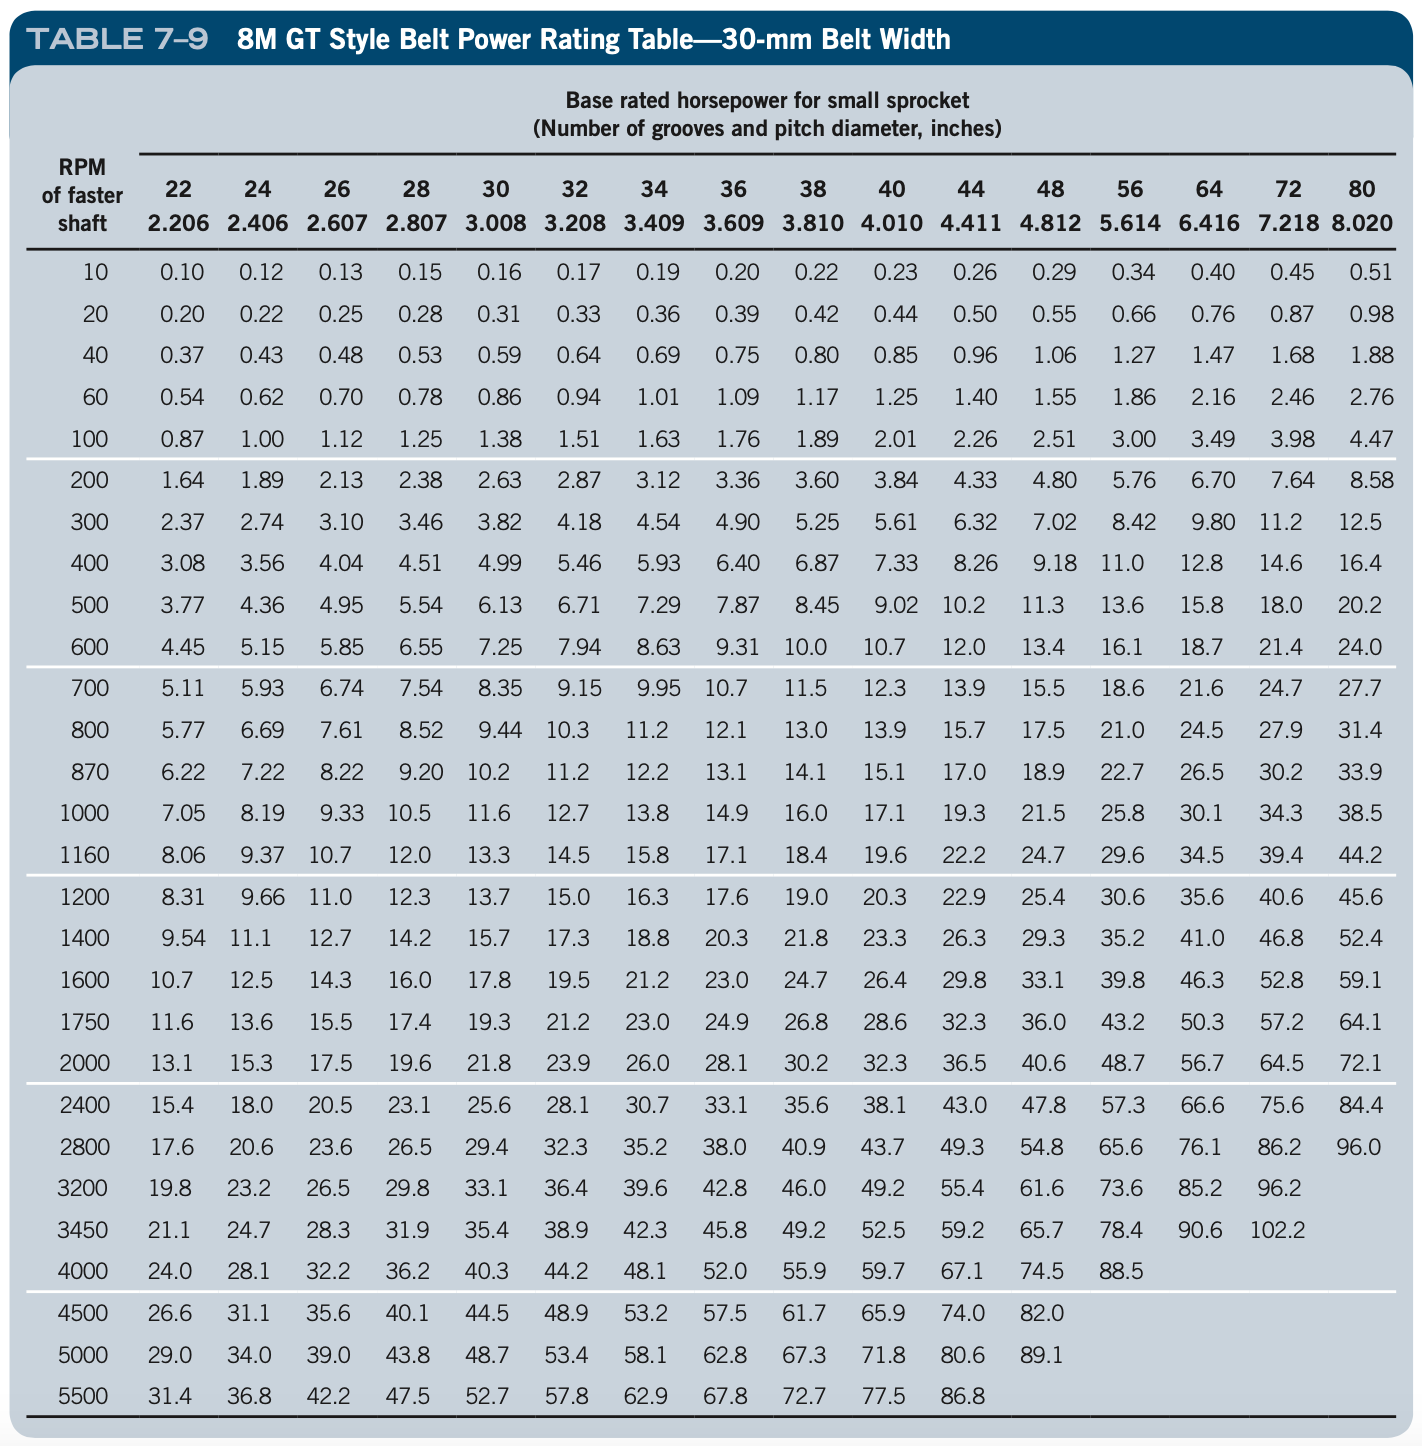
\includegraphics[scale=0.3]{Belts/7-10_pt1.png}\\
    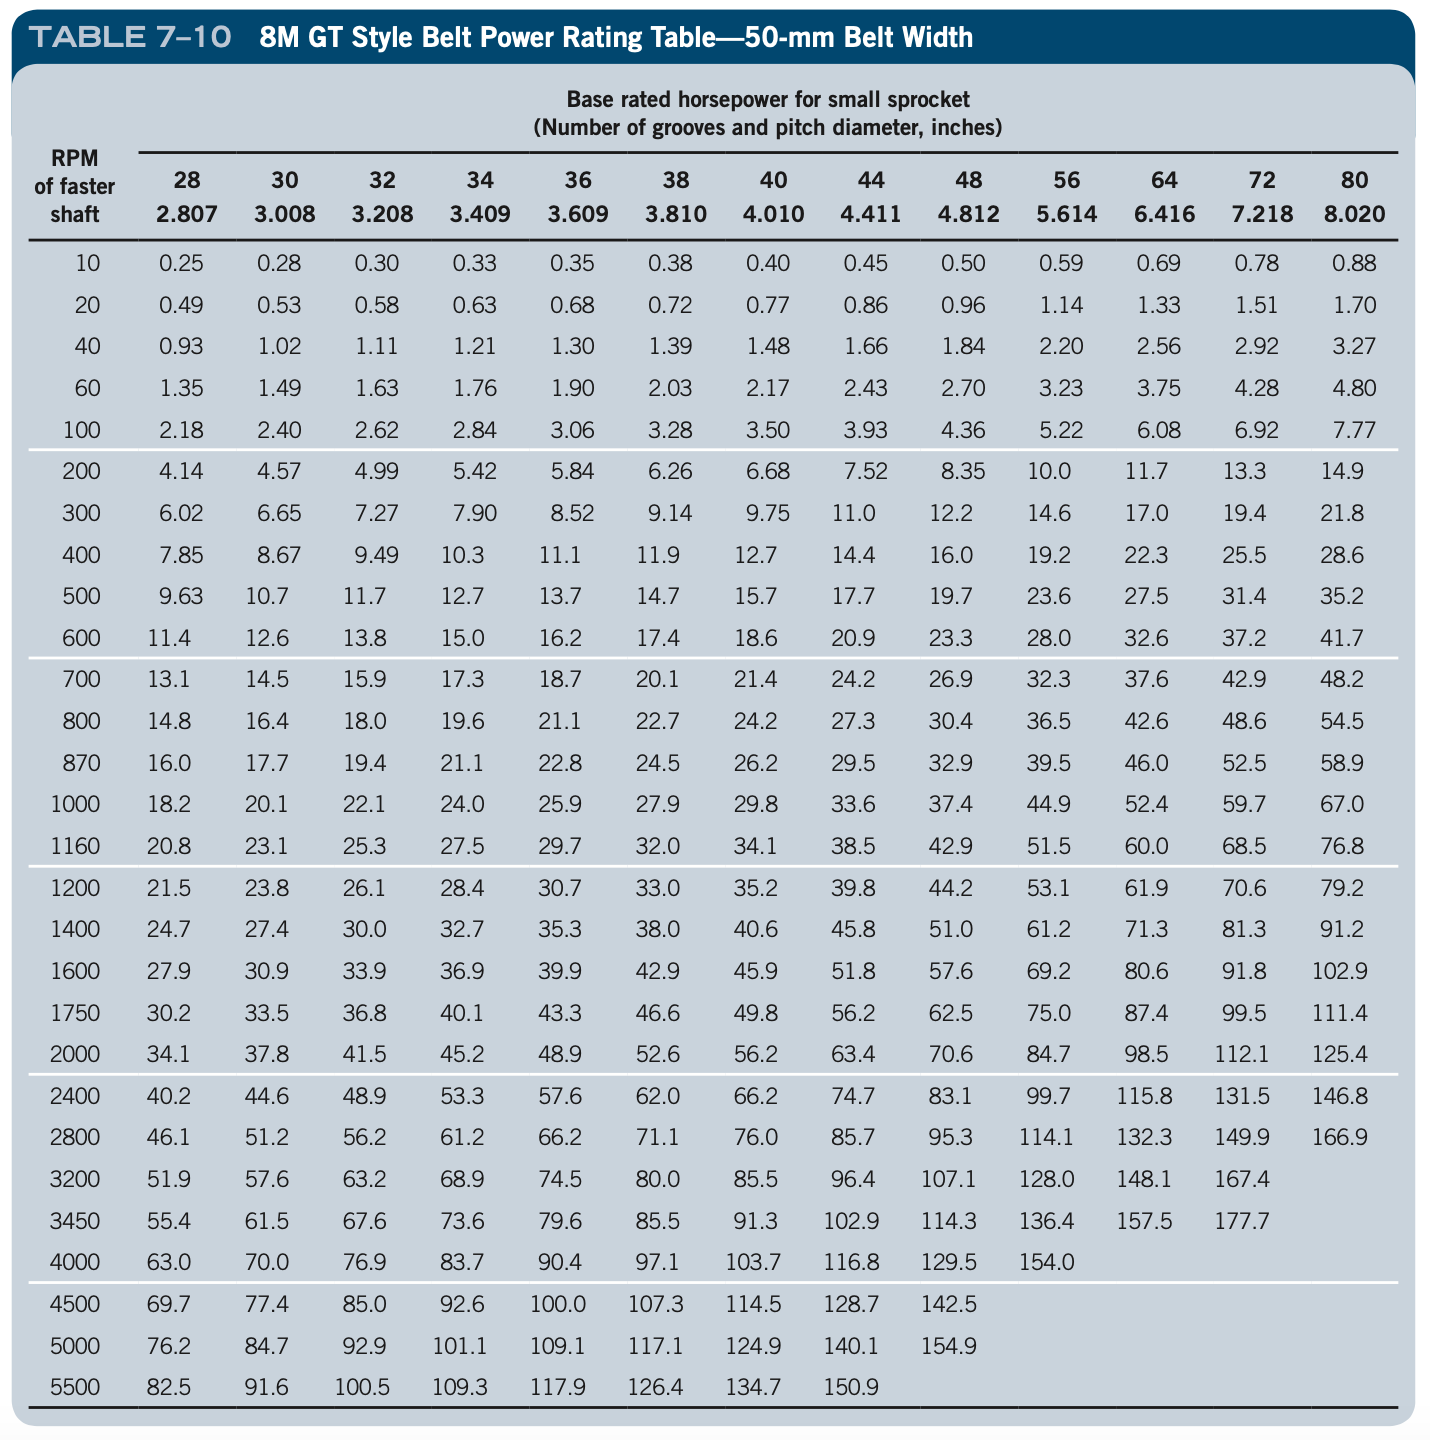
\includegraphics[scale=0.65]{Belts/7-10_pt2.png}
    \item Find belt length correction factor ($C_L$).\\
    If you can't remember the pitch/length designation for your chosen belt, take a look back at table 7-7, they are listed there.\\
    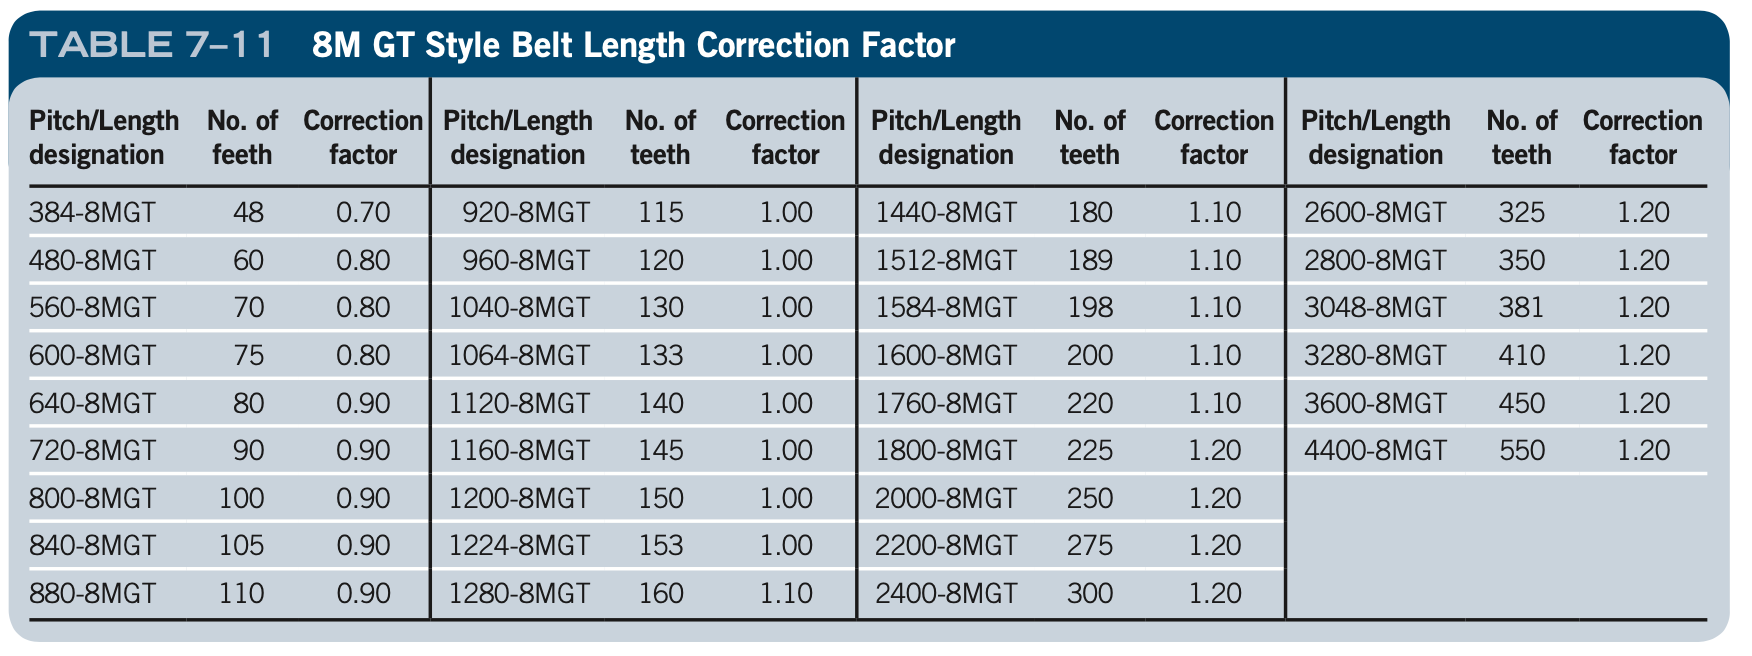
\includegraphics[scale=0.25]{Belts/7-11.png}
    \item Compute the adjusted rated power using $P_{rated}$ found from the table\\
    \begin{align*}
        P_{adj}=P_{rated}\cdot C_L
    \end{align*}
    It's fine if the value is very different than $P_{des}$ found earlier.
    \item Calculate belt speed to ensure it does not exceed 6500 ft/min
    \begin{align*}
        v_{belt}=\frac{PD_1}{2}\cdot \omega_1 \cdot 2\pi\text{ rad/rev}\cdot\frac{1\text{ ft}}{12 \text{ in}}
    \end{align*}
If you get an acceptable belt speed, congrats, you're done!
    
\end{enumerate}

\subsection{Chain Drives}
\subsubsection{Anatomy}
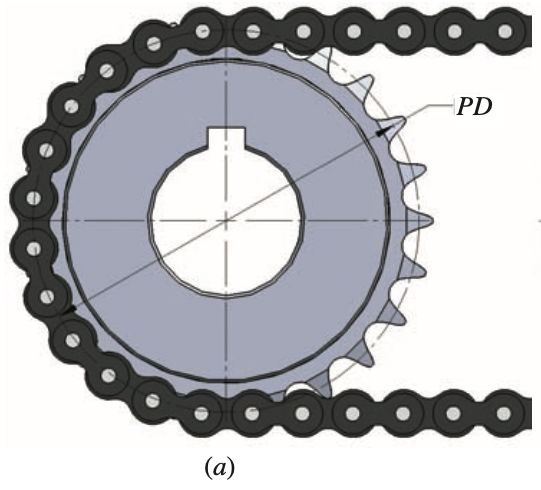
\includegraphics[scale=0.3]{Belts/chain-drive_pd.png}
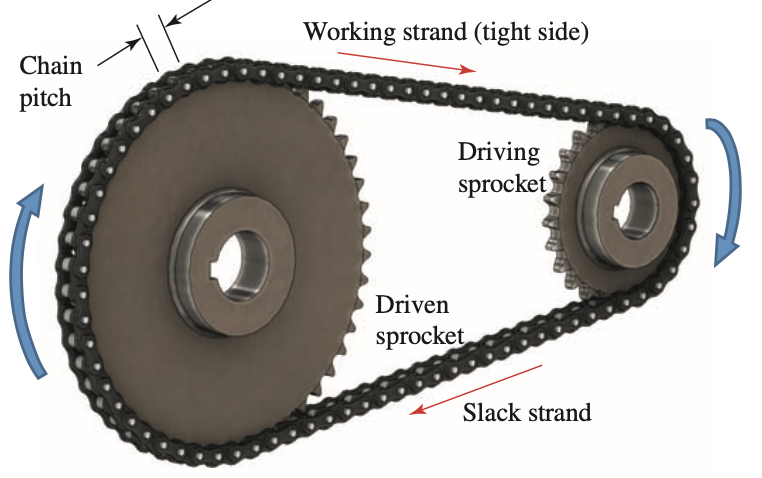
\includegraphics[scale=0.7]{Belts/chain-drives.png}\\
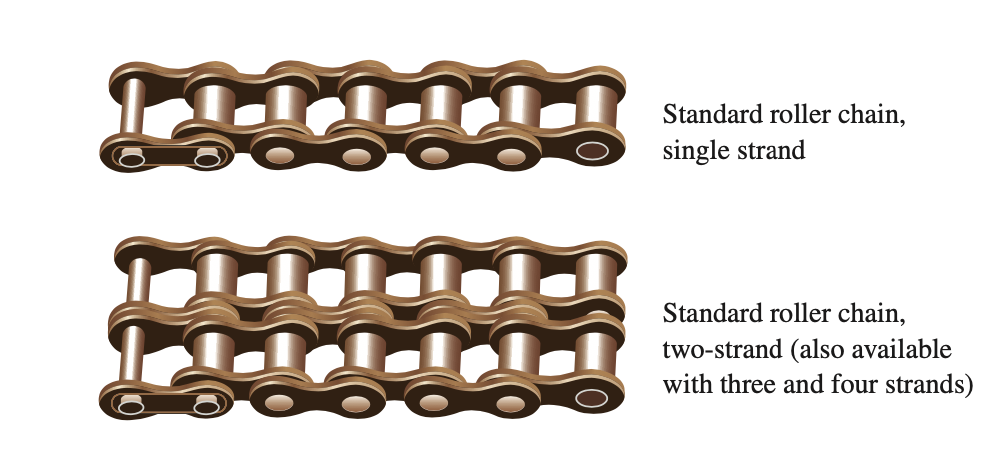
\includegraphics[scale=0.6]{Belts/chains.png}

\subsubsection{Design Selection}
Here are the US standard chains and their tensile strengths:\\
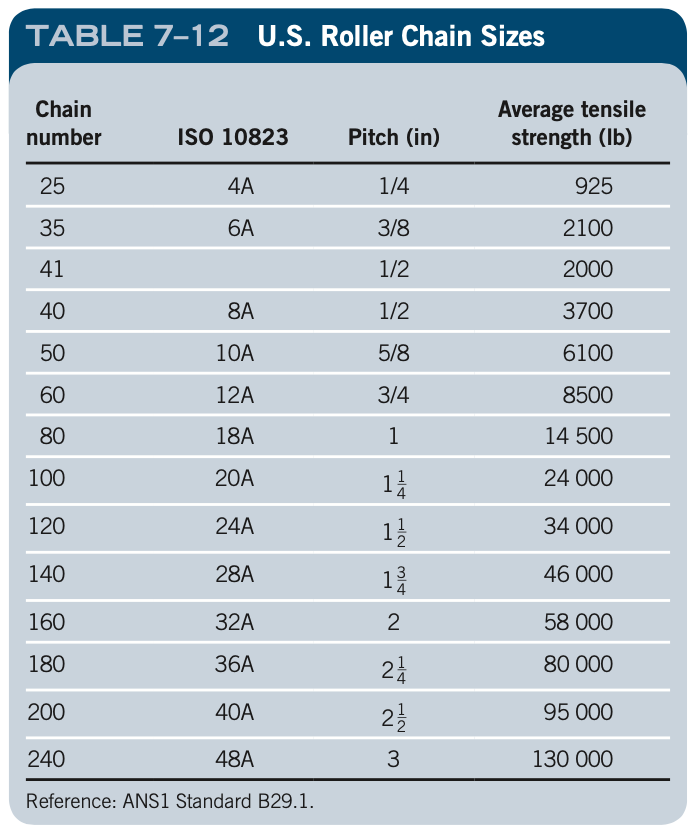
\includegraphics[scale=0.35]{Belts/us-chains.png}\\
If these chains are used to support a load or apply a tensile force, only 10$\%$ of the average tensile strength should be used.

\begin{enumerate}
    \item Determine the service factor and compute the design power\\
    \begin{enumerate}
        \item Get the service factor from this table:\\
        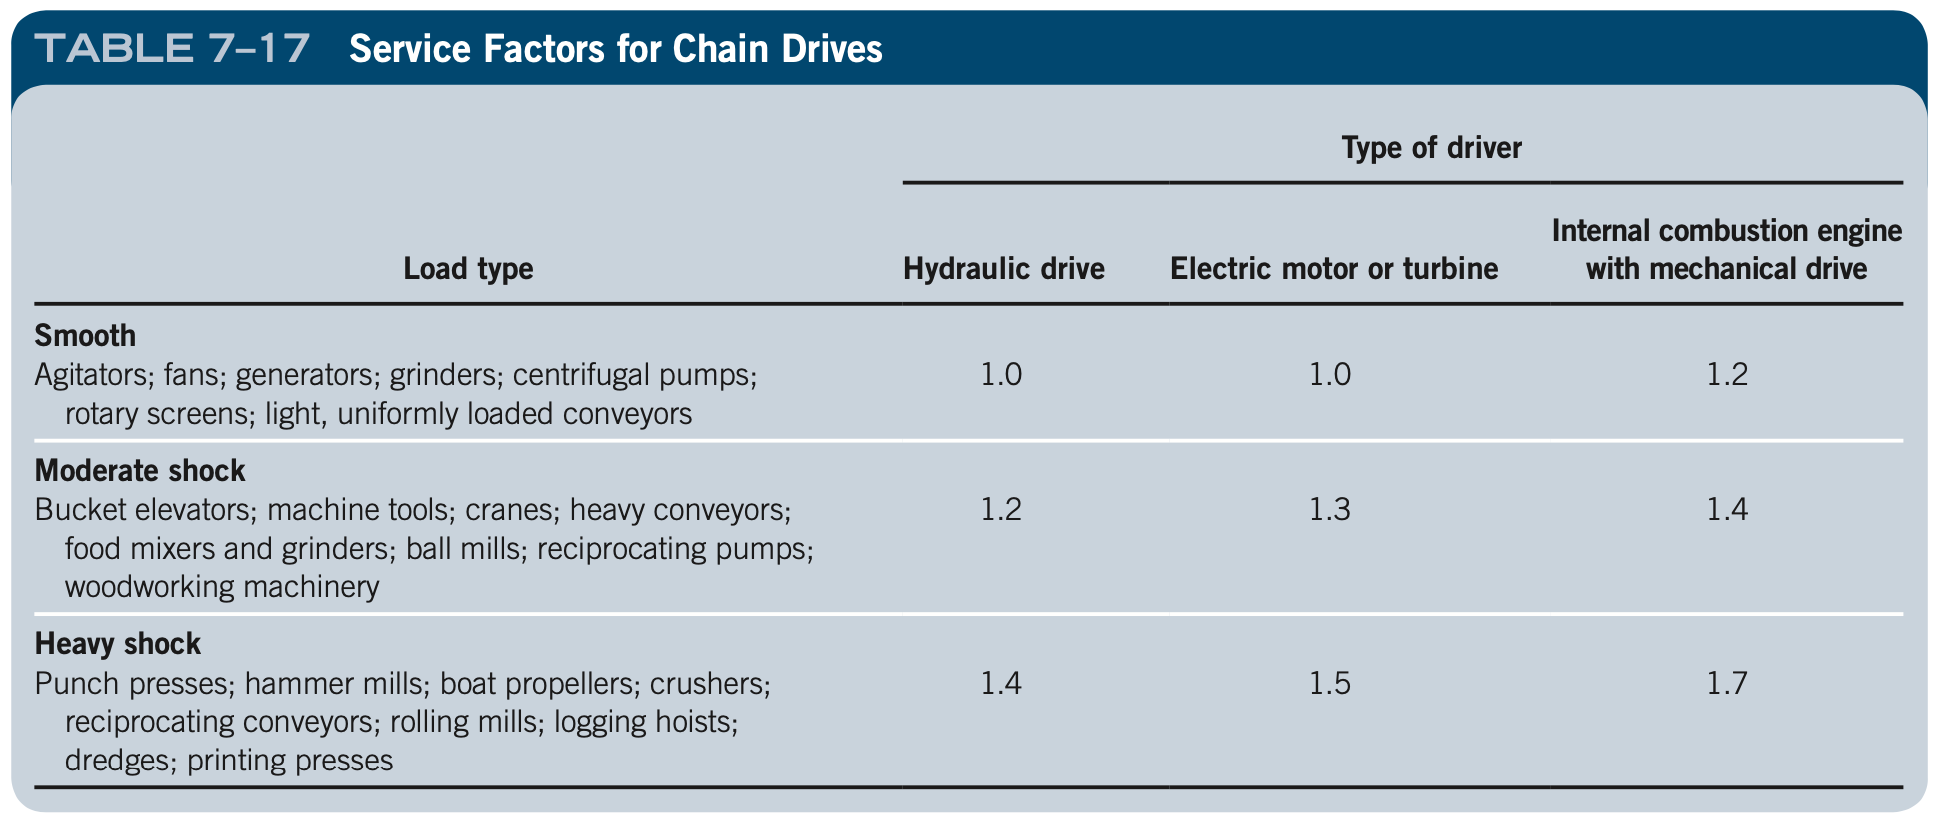
\includegraphics[scale=0.45]{Belts/chain-service.png}
        \item Calculate the design power using $P_{des}=SF\cdot P_{in}$
    \end{enumerate}
    \item Compute the velocity ratio. If you're given an acceptable range for the output speed, use the middle of the range.
    \begin{align*}
        VR=\frac{n_1}{n_2}\text{ where $n_1 > n_2$}
    \end{align*}
    \item Select the chain pitch ($p$) and number of teeth for the small sprocket ($N_1$) using $n_1$. This will also give you the rated power ($P_{rated}$). Refer to the following tables.\\
    A few things to keep in mind:\\
    \begin{enumerate}
        \item You can use a multi-strand design (2, 3 or 4 strands) if you want to use a smaller drive but still transmit the same power at the same speed. To find the required power per stand, use the following power capacity factors:\\
        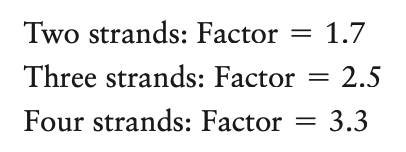
\includegraphics[scale=0.4]{Belts/power-capacity.png}\\
        The required power per chain is then $P_{des}/\text{factor}$
        \item $P_{rated}$ obtained from the tables must be greater than $P_{des}$
        \item The minimum number of teeth in a sprocket should be 17 (unless the it is operation at $<100\text{rpm}$
        \item The largest sprocket should have no more than 120 teeth, so make sure that $(N_1)(VR) < 120$ when selecting $N_1$
        \item You will sadly need to use interpolation to find the rated power if $n_1$ isn't on the table already
        \item The table will also give you the lubrication type
    \end{enumerate}
    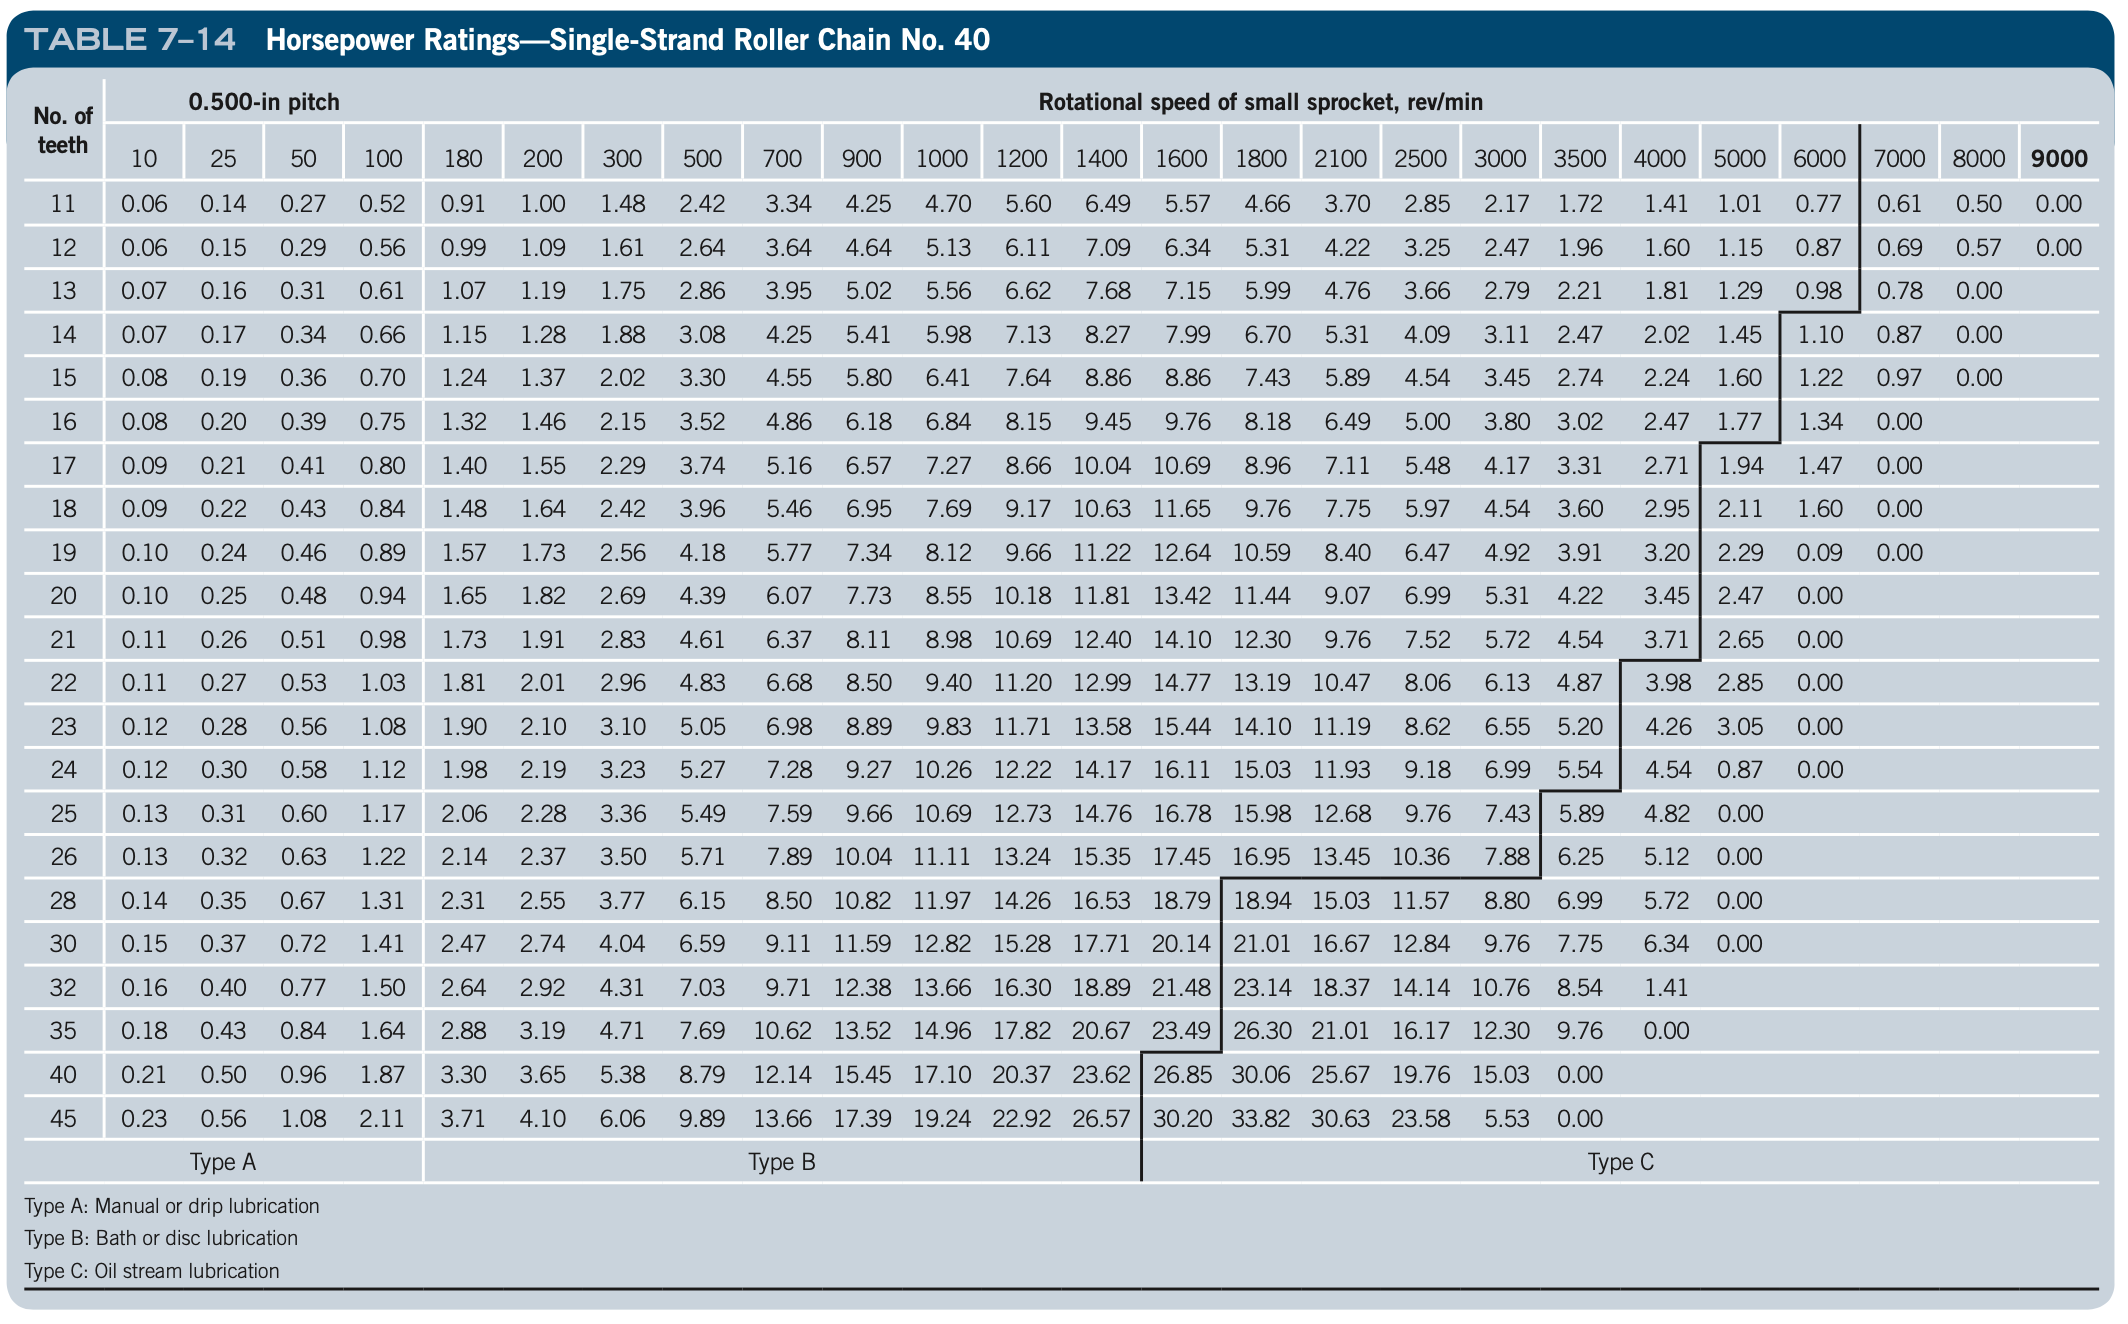
\includegraphics[scale=0.45]{Belts/7-14.png}\\
    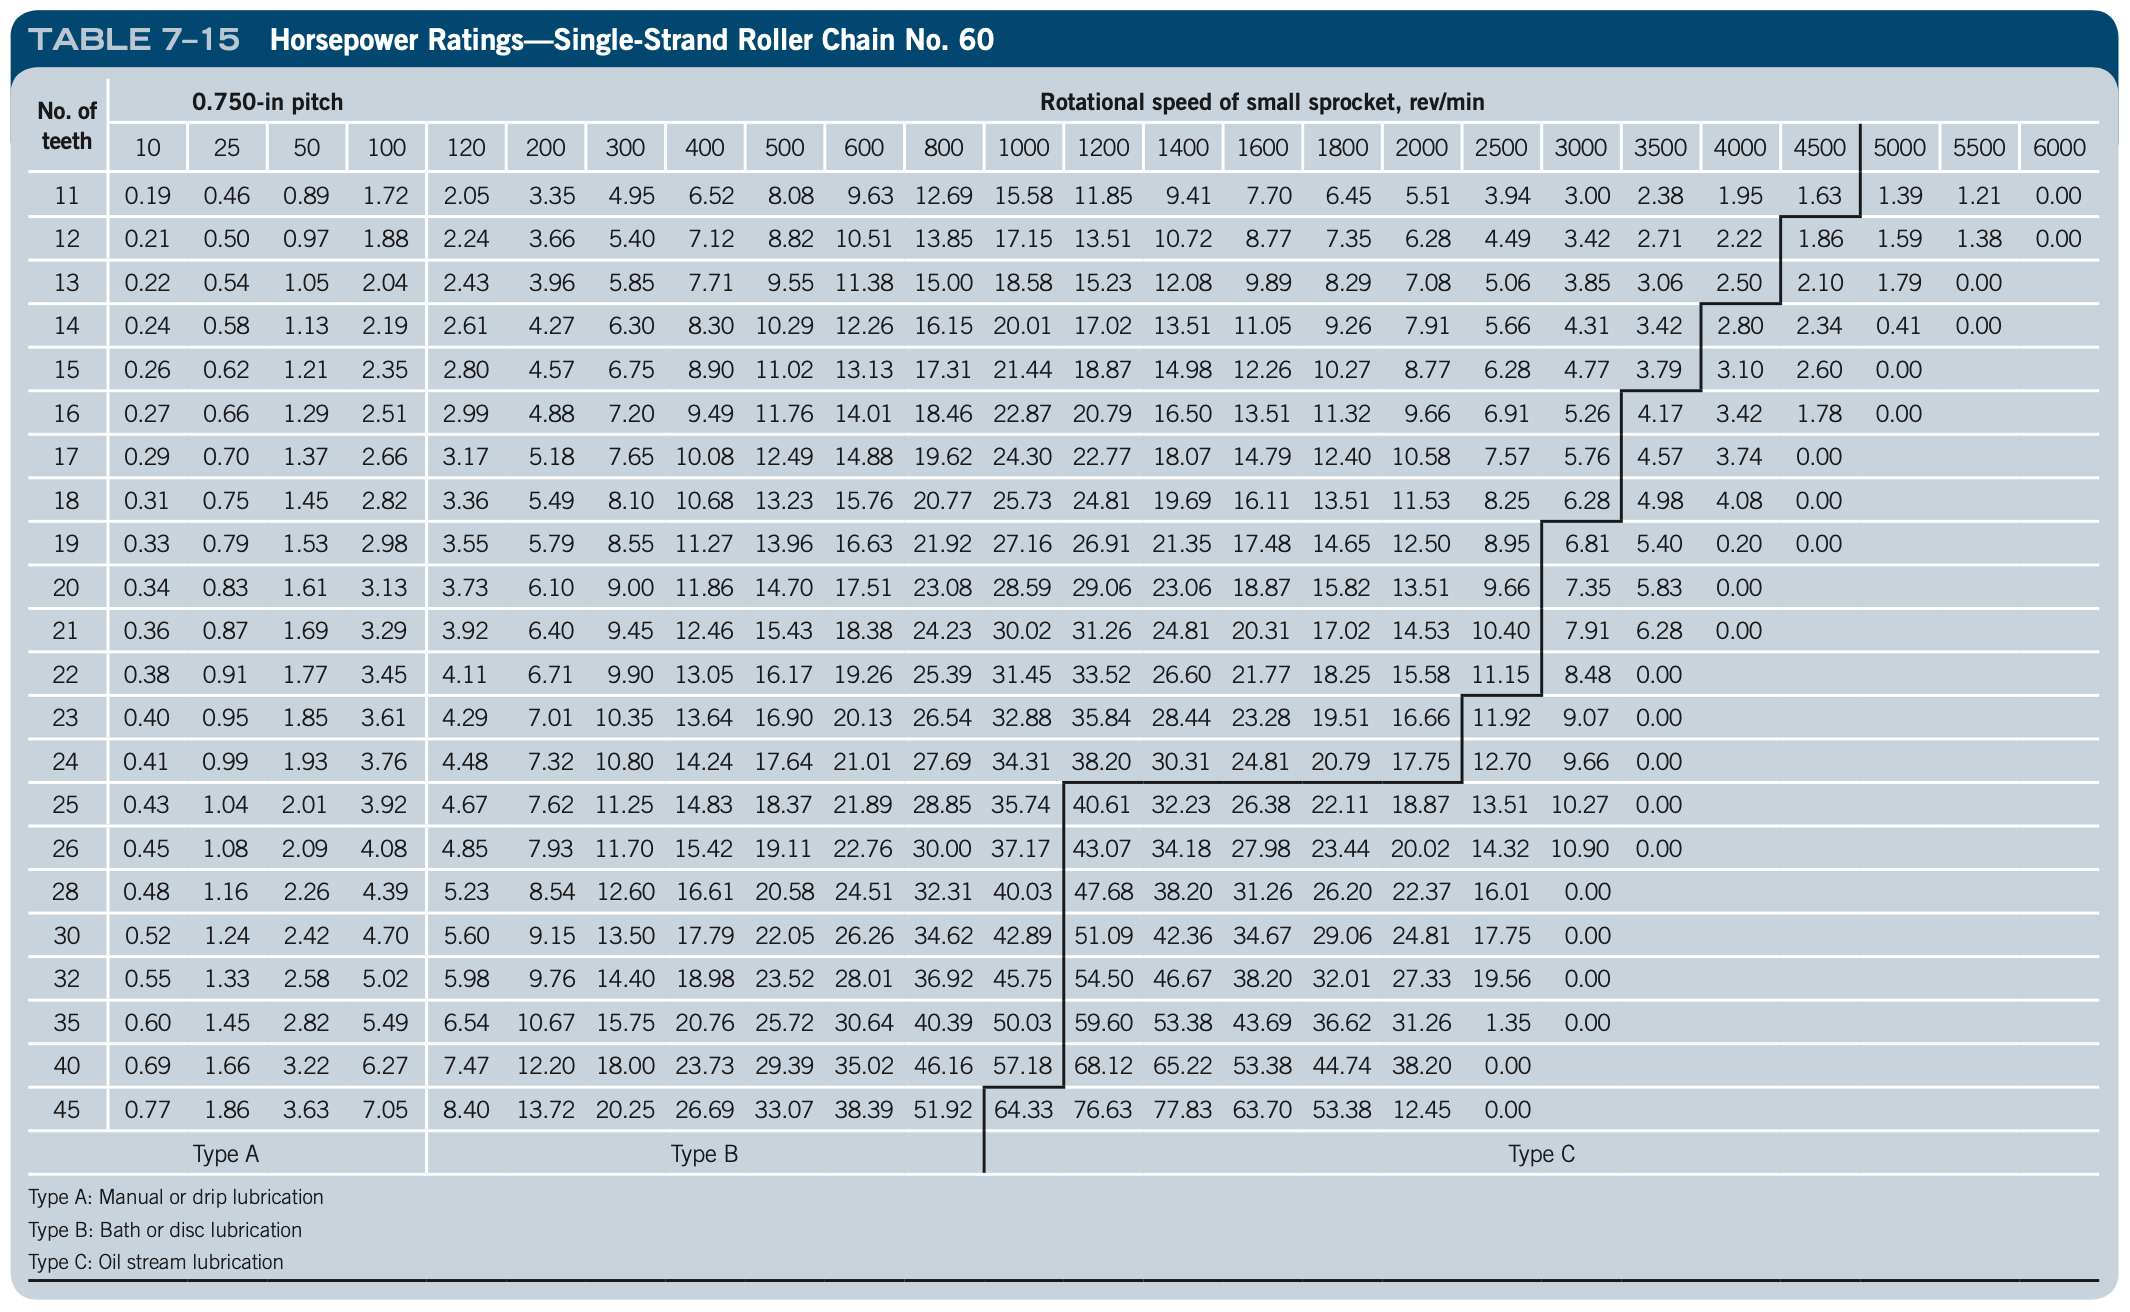
\includegraphics[scale=0.45]{Belts/7-15.png}\\
    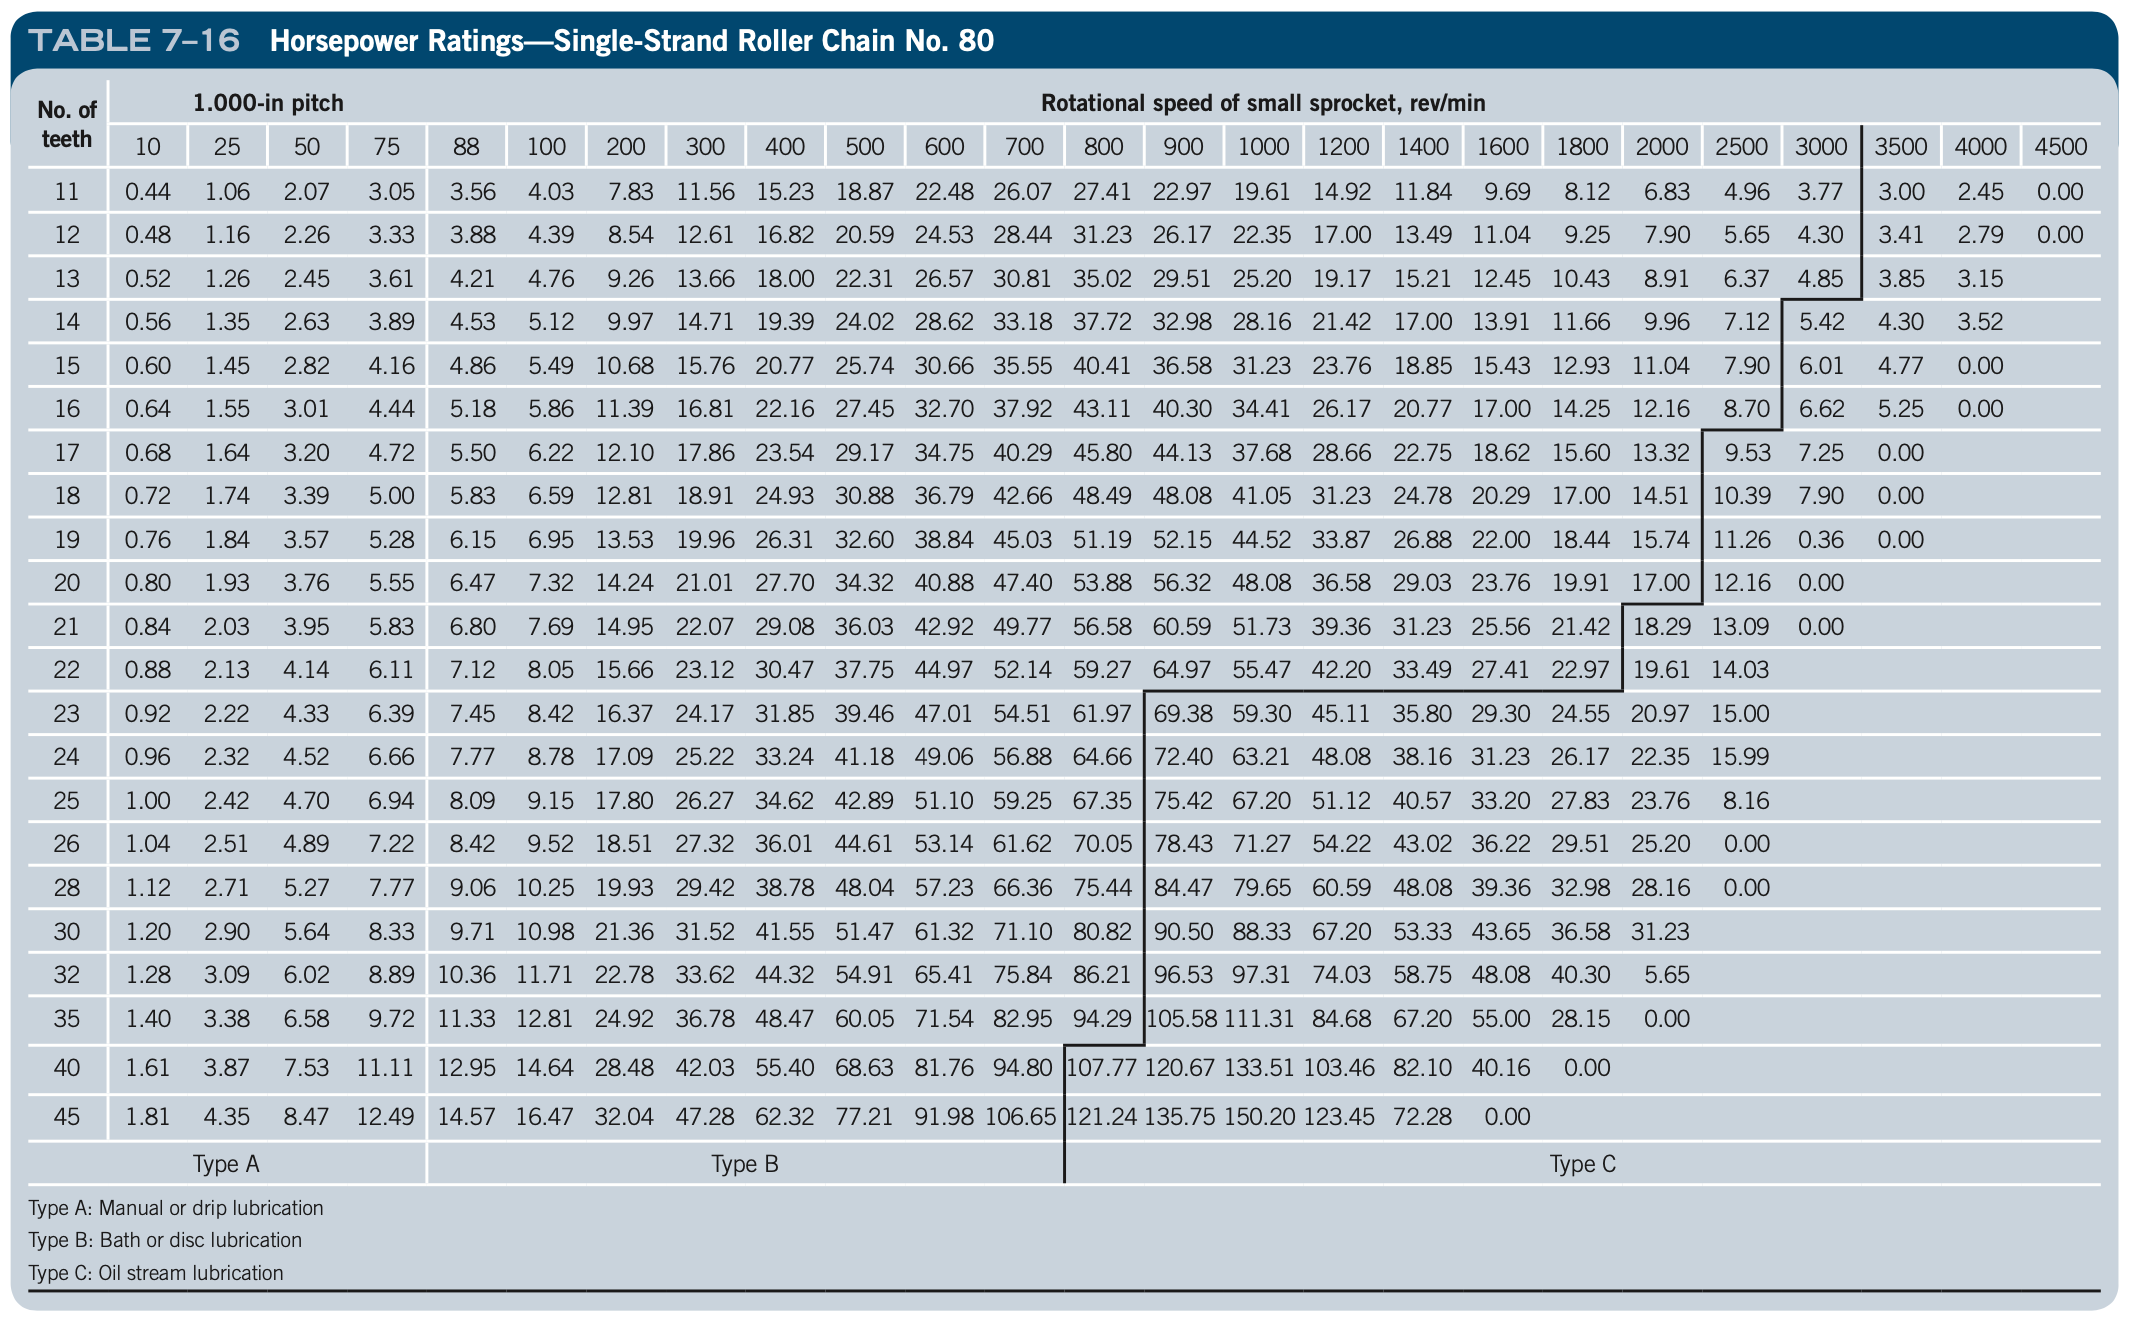
\includegraphics[scale=0.45]{Belts/7-16.png}
    \item Compute the number of teeth on the large sprocket $N_2$:
    \begin{align*}
        N_2=(N_1)(VR)
    \end{align*}
    Round to the nearest integer
    \item Compute the actual output speed and make sure it's in the right range (if a range was given)
    \begin{align*}
        n_2=n_1(N_1/N_2)
    \end{align*}
    \item Compute the pitch diameters of the sprockets
    \begin{align*}
        PD_1=\frac{p}{\sin{(180^{\circ}/N_1)}}\\
        PD_2=\frac{p}{\sin{(180^{\circ}/N_2)}}
    \end{align*}
    Where $p$ is the chain pitch selected in step 3
    \item Specify the nominal CD. The recommended range is 30 to 50 pitches, so let's specify 40 pitches.
    \item Compute the required chain length in pitches
    \begin{align*}
        L_C=2CD+\frac{N_2+N_1}{2}+\frac{(N_2-N_1)^2}{4\pi^2CD}
    \end{align*}
    The chain length must be an integer multiple of the pitch, so round to the nearest integer value
    \item Compute the actual CD
    \begin{align*}
        CD=\frac{1}{4}[L_C-\frac{N_2+N_1}{2}+\sqrt{(L_C-\frac{N_2+N_1}{2})^2-\frac{8(N_2-N_1)^2}{4\pi^2}}]
    \end{align*}
    \item Compute the angle of wrap for each sprocket. The minimum angle of wrap should be $120^\circ$
    \begin{align*}
        \theta_1=180^{\circ}-2\sin^{-1}[\frac{PD_2-PD_1}{2CD}]\\
        \theta_2=180^{\circ}+2\sin^{-1}[\frac{PD_2-PD_1}{2CD}]
    \end{align*}
    \item Compute factor of safety
    \begin{align*}
        FS = P_{allowed}/P_{des}
    \end{align*}
    $P_{allowed}$ is the number you got from the table in step 3 times the strand factor
\end{enumerate}

\subsection{Wire Rope}
\subsubsection{Anatomy}
There's two types of rope winding:\\
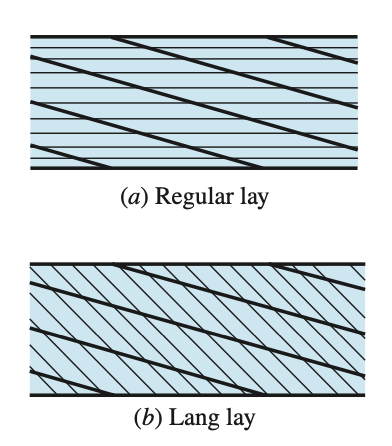
\includegraphics[scale=0.8]{Belts/types-of-rope.png}
\begin{itemize}
    \item Regular-lay ropes have the wires in the strand twisted in one direction and the strands in the rope twisted in the opposite direction
    \item Lang-lay ropes have the wires in the strand and the strands in the rope twisted in the same direction. Lang lay is more flexible than regular lay.
\end{itemize}
\subsubsection{Nomenclature}
$F=$ tensile force on rope (lbf)\\
$W=$ weight at the end of the rope (load) (lbf)\\
$m=$ number of ropes supporting load\\
$w=$ weight/foot supporting load (lbf/ft)\\
$l=$ maximum suspended length of rope (ft)\\
$a=$ maximum acceleration/deceleration ($ft/s^2$)\\
$g=$ acceleration of gravity (32.17 $ft/s^2$)\\
$p/S_u=$ specified life\\
$S_u=$ ultimate tensile strength (psi)\\
$D=$ sheave or which drum diameter (in)\\
$d=$ nominal wire rope size (in)\\
$E_r=$ Young's modulus (psi)\\
$d_w=$ diameter of the wire (in)\\
$A_m=$ metal cross-sectional area ($in^2$)\\

\subsubsection{Formulae}
\begin{align*}
    \text{rope tension: }& F_t=\brround{\frac{W}{m}+wl}\brround{1+\frac{a}{g}}\\
    \text{ultimate strength of wire: }& S_u = \frac{2000F}{Dd}\\
    \text{fatigue tension: }& F_f=\frac{(p/S_u)S_uDd}{2}\\
    \text{equivalent bending load: }& F_b=\frac{E_rd_wA_m}{D}\\
    \text{fatigue factor of safety: }& n_f=\frac{F_f-F_b}{F_t}\\
    \text{factor of safety for static loading: }& n_s=\frac{F_u-F_b}{F_t}\\
    \text{bearing pressure: }& P=\frac{2F}{dD}
\end{align*}
\subsubsection{Useful Tables}
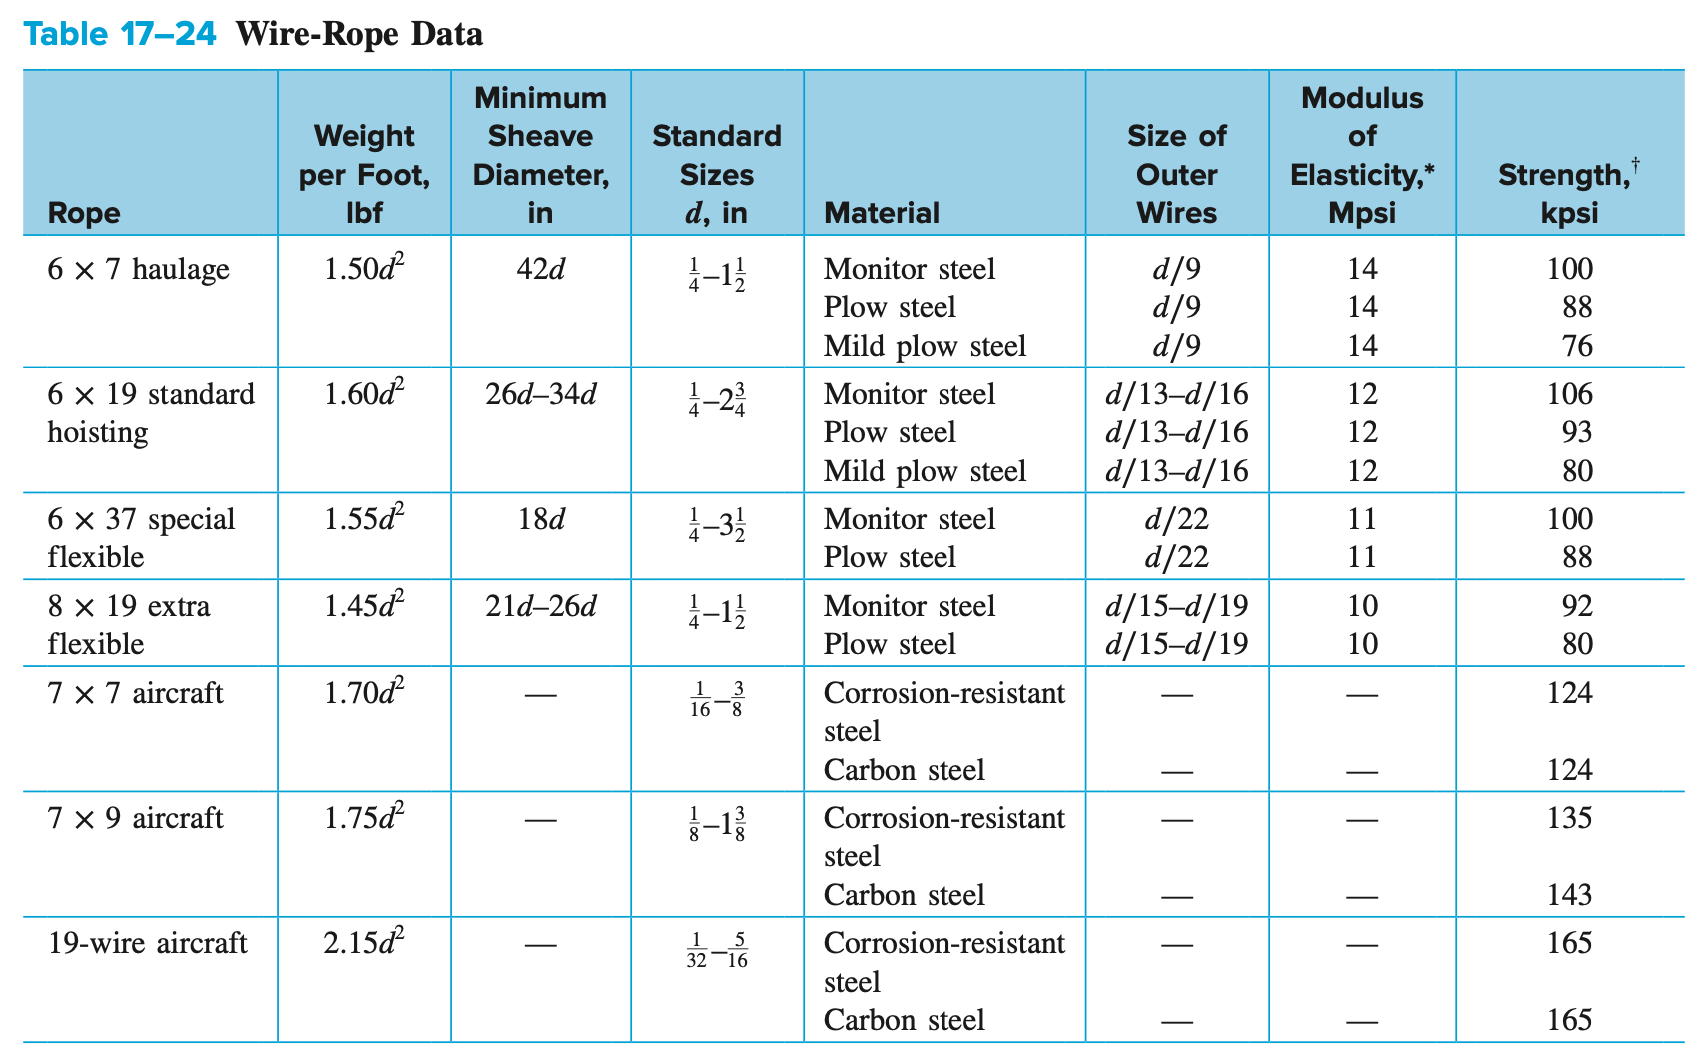
\includegraphics[scale=0.6]{Belts/wire-rope_data.png}\\
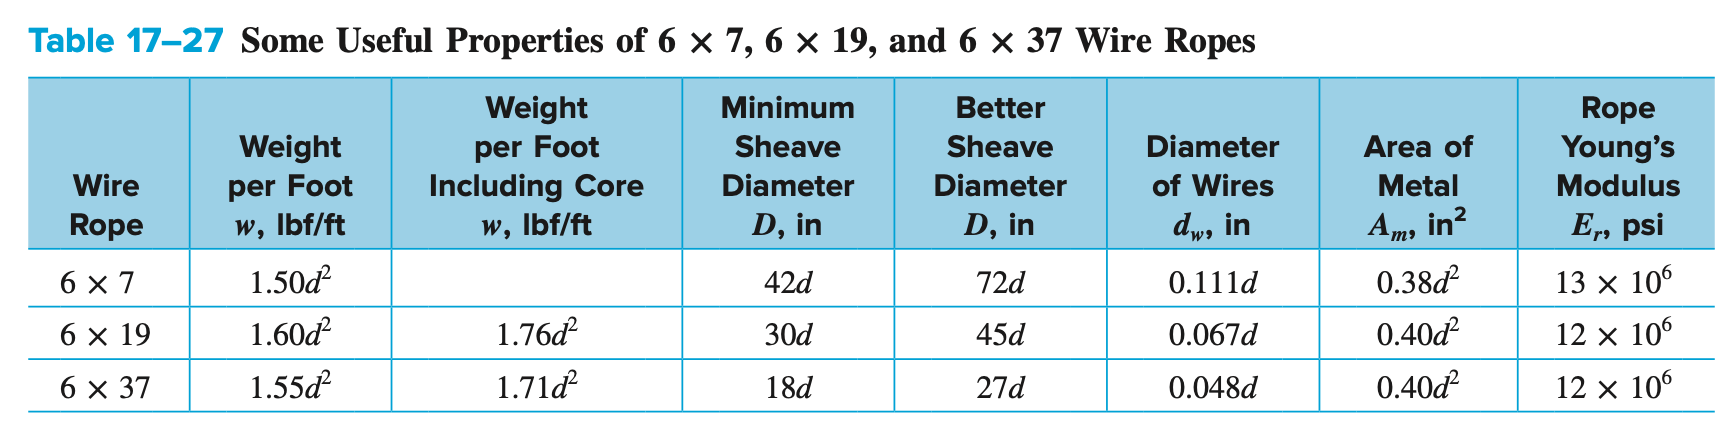
\includegraphics[scale=0.6]{Belts/17-27.png}\\
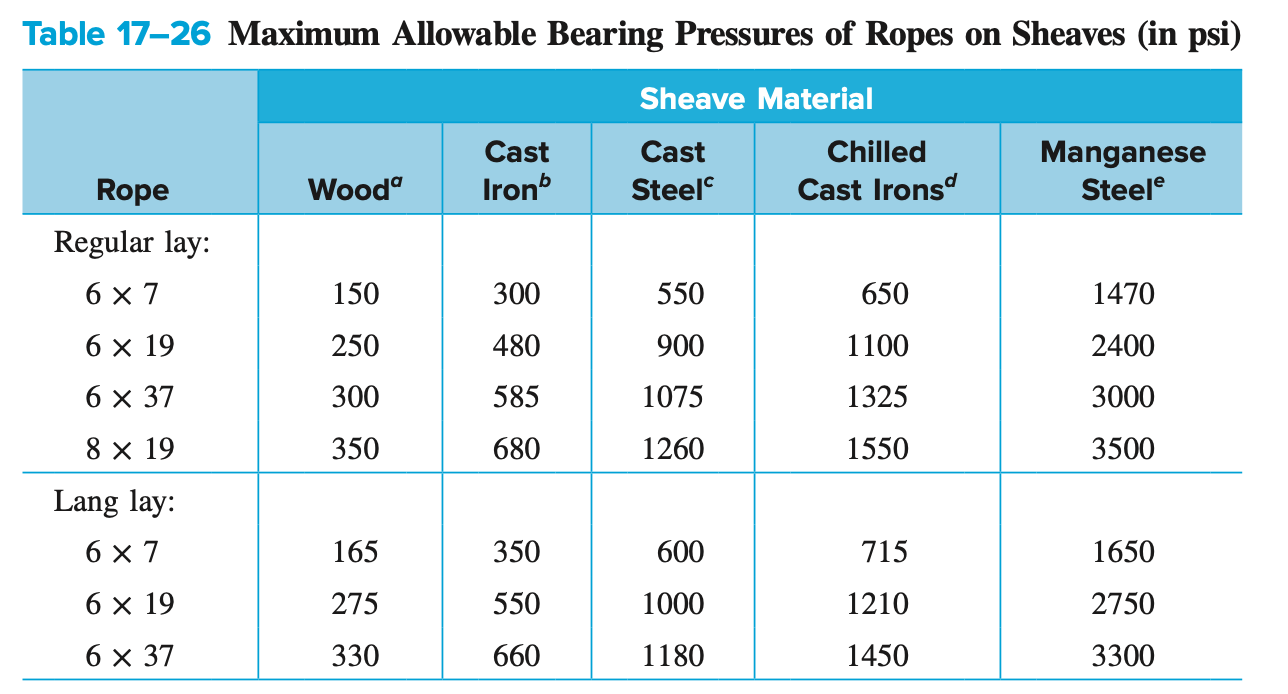
\includegraphics[scale=0.6]{Belts/max-allowable-pressure.png}\\
$S_u$ ranges:\\
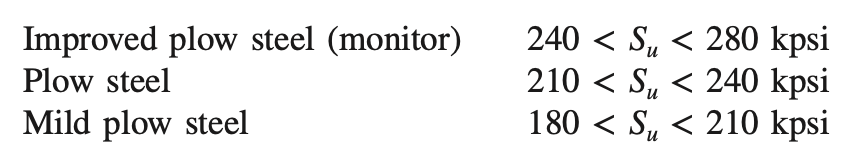
\includegraphics[scale=0.6]{Belts/S_u.png}\\
No idea how to use this but here it is in case it's relevant:\\
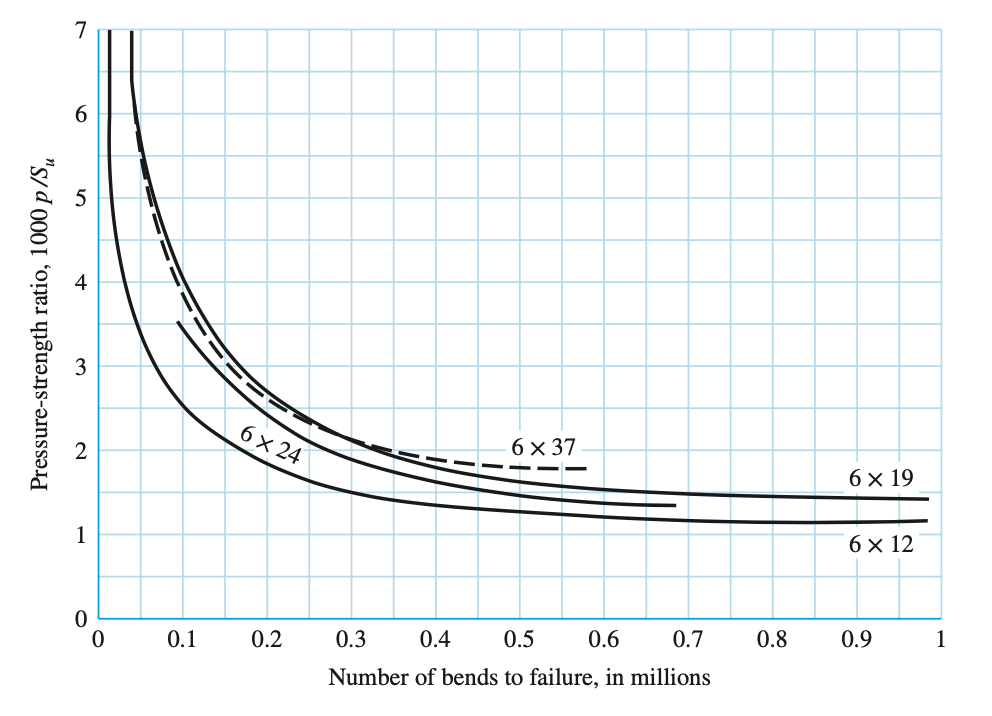
\includegraphics[scale=0.75]{Belts/dumb_table.png}
\section{Gears and Shit}



\subsection{Spur Gears}
\subsubsection{Anatomy}
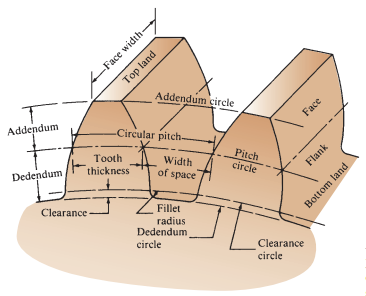
\includegraphics[scale=0.9]{Gears/Diagram.png}
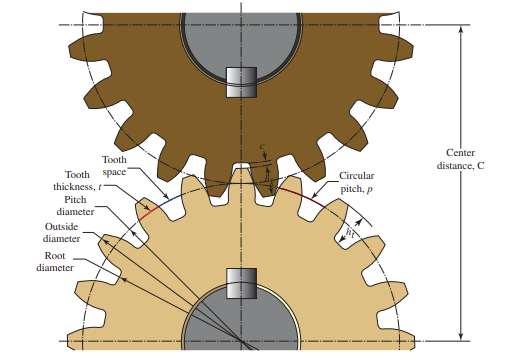
\includegraphics[scale=0.9]{Gears/TwoGearDiagram.png}
\subsubsection{Nomenclature}
``pinion" is the smaller gear\\
``gear" is the larger gear\\
$N_P=$ number of teeth on pinion (input)\\
$N_G=$ number of teeth on gear (output)\\
$p=$ circular pitch (in)\\
$P_d=$ diametral pitch (teeth/in)\\
$m=$ module (in/teeth)\\
$D_P=$ pitch diameter of pinion (in)\\
$D_G=$ pitch diameter of gear (in)\\
$D_o=$ outside diameter (in)\\
$D_R=$ root diameter (in)\\
$D_b=$ base circle diameter (in)\\
$R=\frac{D}{2}=$ radius (in)\\
$a=$ addendum (in)\\
$b=$ dedendum (in)\\
$c=$ clearance (in)\\
$h_f=$ whole depth (in)\\
$h_k=$ working depth (in)\\
$t=$ tooth thickness (in)\\
$F=$ face width (in)\\
$\phi=$ pressure angle\\
$C=$ center distance (in)\\
$m_f=$ contact ratio\\
$m_G=$ gear ratio\\
$n_P=$ pinion speed (input) (rpm)\\
$n_G=$ gear speed (output) (rpm)\\
$W_t=$ transmitted load (lbf)\\
$W_r=$ radial force (lbf)\\
$W_n=$ normal force (lbf)\\
$H=P=$ transmitted power (hp)\\
$V=v_t=$ pitch-line velocity (ft/min)\\
$F_{x,y}^t=$ transmitted force between gears $x$ and $y$ (lbf)\\
$F_{x,y}^r=$ radial force between gears $x$ and $y$ (lbf)\\
$T=$ torque ($\mathrm{lbf\cdot in}$)\\
$K_O=$ Overload Factor\\
$P_\text{des}=$ design power (hp)\\
$VR=$ velocity ratio\\
$C_P=$ elastic coefficient\\
$A_v=$ quality number\\
$K_v=$ dynamic factor\\
$J_P=$ bending geometry factor of the pinion\\
$J_G=$ bending geometry factor of the gear\\
$I=$ pitting geometry factor\\
$C_{pf}=$ pinion proportion factor\\
$C_{ma}=$ mesh alignment factor\\
$K_m=$ load-distribution factor\\
$K_s=$ size factor\\
$K_B=$ rim thickness factor\\
$FS=$ service factor\\
$K_R=$ reliability factor\\
$N_{cP}=$ number of loading cycles for pinion\\
$N_{cG}=$ number of loading cycles for gear\\
$Y_{NP}=$ bending stress cycle factor for pinion\\
$Y_{NG}=$ bending stress cycle factor for gear\\
$Z_{NP}=$ pitting resistance stress cycle factor for pinion\\
$Z_{NG}=$ pitting resistance stress cycle factor for gear\\
$s_{tP}=$ expected bending stress in pinion (psi)\\
$s_{tG}=$ expected bending stress in gear (psi)\\
$s_{atP}=$ adjusted expected bending stress in pinion (psi)\\
$s_{atG}=$ adjusted expected bending stress in gear (psi)\\
$s_c=$ expected contact stress\\
$s_{cP}=$ adjusted expected contact stress for pinion\\
$s_{cG}=$ adjusted expected contact stress for gear

\subsubsection{Formulae}
Geometry:
\begin{align*}
    \text{circular pitch: }&p=\frac{\pi D_P}{N_P}=\frac{\pi D_G}{N_G}=\frac{\pi}{P_d}\\
    \text{diametral pitch: }&P_d=\frac{N_P}{D_P}=\frac{N_G}{D_G}=\frac{\pi}{p}\\
    \text{module: }&m=\frac{D_P}{N_P}=\frac{D_G}{N_G}=\frac{1}{P_d}\\
    \text{gear ratio: }&m_G=\frac{N_G}{N_P}\\
    \text{outside diameter: }&D_o=\frac{N+2}{P_d}\\
    \text{root diameter: }&D_R=D-2b\\
    \text{addendum: }&a=\frac{1}{P_d}\\
    \text{dedendum: }&b=\eqnsystem{\frac{1.25}{P_d} & P_d<20\\ \frac{1.20}{P_d}+0.002 & P_d\geq 20}\\
    \text{clearance: }&c=\eqnsystem{\frac{0.25}{P_d} & P_d<20\\ \frac{0.2}{P_d}+0.002 & P_d\geq 20}\\
    \text{whole depth: }&h_f=a+b\\
    \text{working depth: }&h_k=2a\\
    \text{tooth thickness: }&t=\frac{p}{2}=\frac{\pi}{2P_d}\\
    \text{nominal face width: }&F=\frac{12}{P_d}\\
    &\frac{8}{P_d}<F<\frac{16}{P_d}\\
    \text{center distance: }&C=\frac{D_P+D_G}{2}=\frac{N_P+N_G}{2P_d}\\
    \text{base circle diameter: }&D_b=\frac{N_p}{P_d}\cos\phi\\
    \text{contact ratio: }&m_f=\frac{\sqrt{R_{oP}^2-R_{bP}^2}+\sqrt{R_{oG}^2-R_{bG}^2}-C\sin\phi}{p\cos\phi}\\
    &F_{\text{driving},x}^t=W_t\\
    &F_{x,y}^r=F_{x,y}^t\tan\phi\\
    &T=\frac{W_td}{2}
\end{align*}
Forces and motion:
\begin{align*}
    \text{pitch line speed(ft/min): }&v_t=\frac{\pi D n}{12}\\
    \text{velocity ratio: }&VR=\frac{n_P}{n_G}=\frac{N_G}{N_P}\\
    \text{torque: }&T=\frac{63000P}{n}=\frac{W_tD}{2}\\
    \text{tangential force: }&W_t=\frac{33000P}{v_t}=\frac{126000P}{nD}\\
    \text{radial force: }&W_r=W_t\tan\phi\\
    \text{normal force: }&W_n=\frac{W_t}{\cos\phi}=\sqrt{W_t^2+W_r^2}\\
    \text{bending stress number: }&s_t=\frac{W_tP_d}{FJ}K_OK_sK_mK_BK_v\\
    \text{contact stress number: }&s_c=C_p\sqrt{\frac{W_tK_OK_sK_mK_v}{FD_pI}}\\
    \text{allowable bending stress: }&s_{at}>s_t\frac{(SF)K_R}{Y_N}\\
    \text{allowable contact stress: }&s_{ac}>s_c\frac{(SF)K_R}{Z_N}
\end{align*}

\subsubsection{Design Selection}
In these 39 simple steps, you too can become a \sout{masochist} Mechanical Engineer!
\begin{enumerate}
    \item Find the type of shock for input and output from this random place in the textbook:\\
    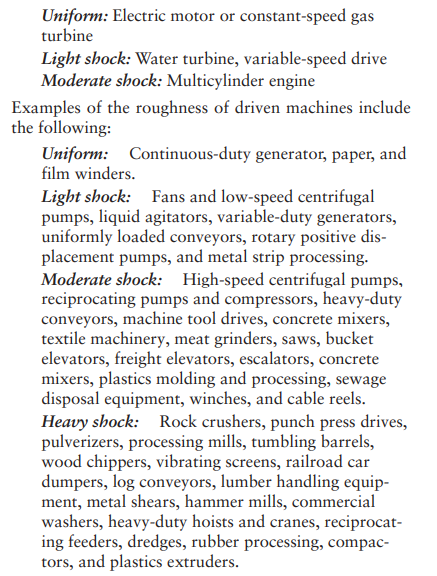
\includegraphics[scale=1]{Gears/Shock.png}
    \item Use this fucking thing to find the shock\\
    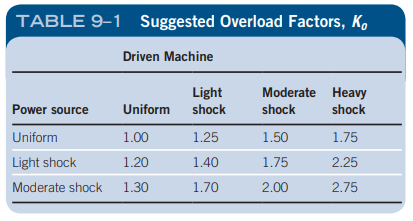
\includegraphics[scale=1]{Gears/9-1.png}
    \item Find $P_\text{des}=PK_O$
    \item Find $P_d$:\\
    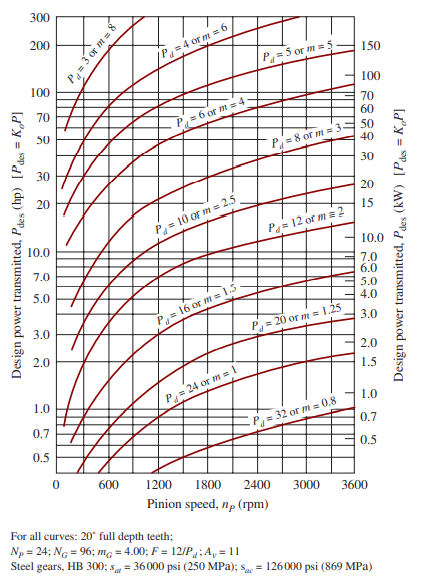
\includegraphics[scale=1]{Gears/Fig 9-11.png}\\
    (round to smallest number)
    \item Choose $N_p$ to be some random fucking value between 17 and 20.
    \item declare what you think $n_G$ should be based on the range in the problem statement. (assume the value is the middle of the acceptable range)
    \item Get the velocity ratio
    \begin{align*}
        &VR=\frac{n_P}{n_G}
    \end{align*}
    \item Compute the number of teeth on the output gear $N_G=N_P(VR)$ (round to nearest int)
    \item Compute the actual velocity ratio
    \begin{align*}
        &VR=\frac{N_G}{N_P}
    \end{align*}
    \item Compute the actual output speed
    \begin{align*}
        &n_G=n_P\brround{\frac{N_P}{N_G}}
    \end{align*}
    Check that it's within the specified range, if not try new Np
    \item Compute the diameters of the gears
    \begin{align*}
        &D_P=\frac{N_P}{P_d}\\
        &D_G=\frac{N_G}{P_d}
    \end{align*}
    \item Compute the center distance, pitch line speed, and transmitted load because why the hell not
    \begin{align*}
        &C=\frac{N_P+N_G}{2P_d}\\
        &v_t=\frac{\pi}{12}D_Pn_P\\
        &W_t=\frac{33000P}{v_t}
    \end{align*}
    \item Find the face width, $F$. Just use the nominal one and don't question where the numbers come from.
    \begin{align*}
        &\text{nominal value}=\frac{12}{P_d}\\
        &\text{lower limit}=\frac{8}{P_d} &0.5<\frac{F}{D_p}<2, \text{ if you are outside this range try a different value}\\
        &\text{upper limit}=\frac{16}{P_d}
    \end{align*}
    \item Choose a material. I have no clue how to do this so just always choose steel and hope it works.\\
    For Material and stress look at table 9-13 on page 401 in Motts\\
    \item Find $C_P$ based on the material. It will be $2300$ for steel\\
    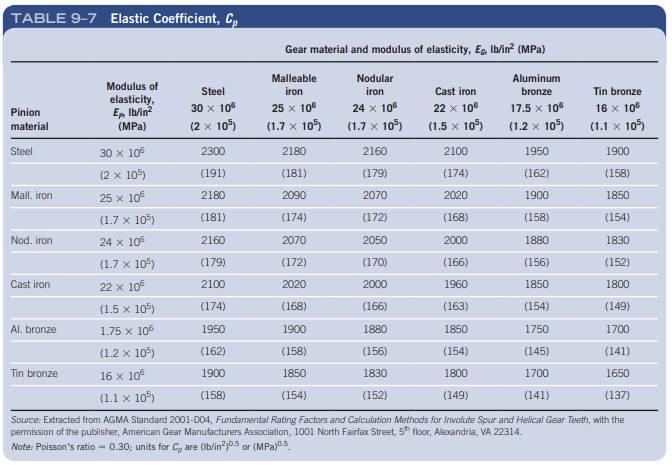
\includegraphics[scale=1]{Gears/9-7.png}
    \item Find the quality number $A_v$ from the application or the pitch line speed. This table is shit so just guess what looks right.\\
    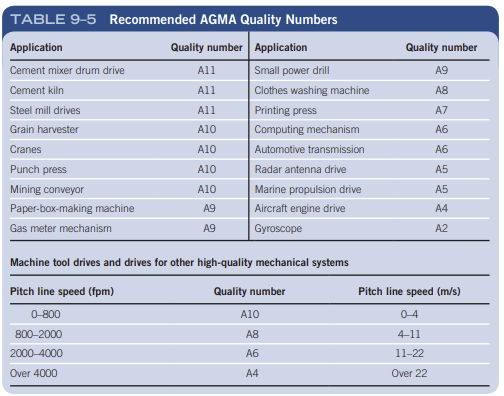
\includegraphics[scale=1]{Gears/9-5.png}
    \item Find the dynamic factor $K_v$ from this graph using $A_v$ and $v_t$\\
    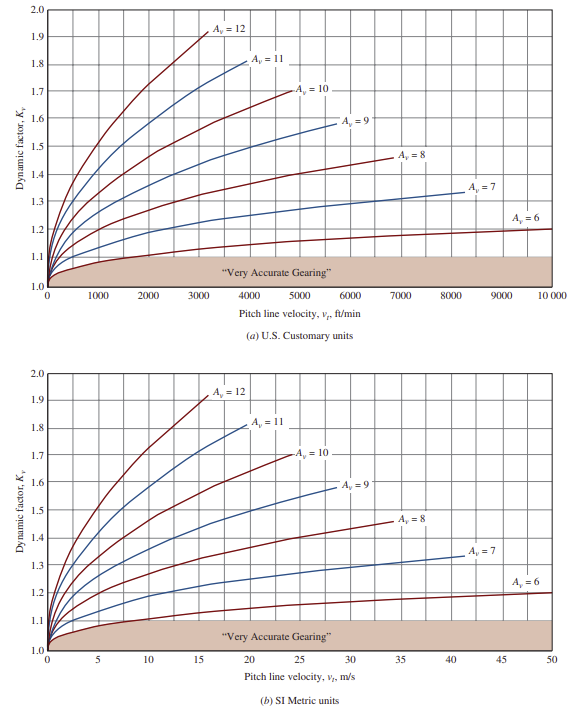
\includegraphics[scale=1]{Gears/Fig 9-16.png}
    \item Choose the $J_P$ and $J_G$ values. Assume $20^\circ$ unless otherwise specified. Why? Because fuck you, that's why.\\
    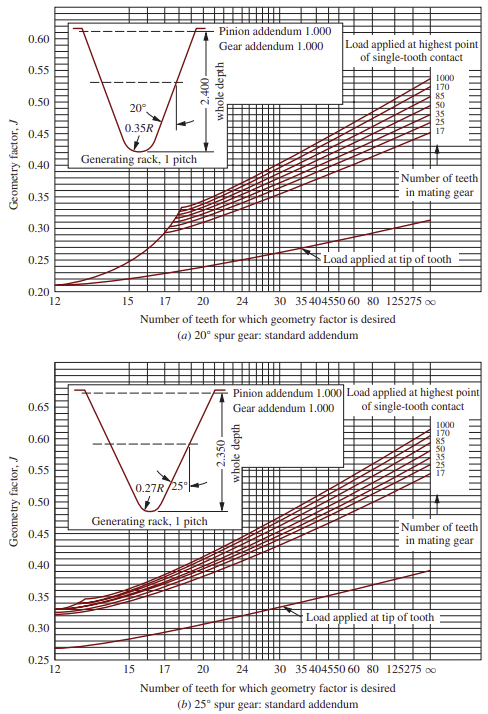
\includegraphics[scale=1]{Gears/Fig 9-10.png}
    \item Choose the pitting geometry factor, $I$. Use the same pressure angle.\\
    \includegraphics[scale=1]{Gears/Fig 9-17.png}
    \item Find $C_{pf}$ from this. Use the equations if you can because the table is bad.\\
    \includegraphics[scale=1]{Gears/Fig 9-12.png}
    \item Find $C_{ma}$ from this. Probably use commercial enclosed gear units but do whatever you feel like.\\
    \includegraphics[scale=1]{Gears/Fig 9-13.png}
    \item Compute $K_m=1+C_{pf}+C_{ma}$
    \item Find $K_s$ from this\\
    \includegraphics[scale=1]{Gears/9-2.png}
    \item Find $K_B$. It will always be 1.00 unless it isn't. If it isn't then use this ugly picture\\
    \includegraphics[scale=1]{Gears/Fig 9-14.png}
    \item Specify a service factor, $SF$ between $1.00$ and $1.50$. Usually pick $1.00$ but if your data is uncertain then ramp that shit up.
    \item Gander a guess at how reliable your system will be. Let's assume for most cases that you're not that shit of an Engineer and it works $99\%$ of the time.
    \item Use your rigorously calculated reliability to get $K_R$ from yet another fucking table\\
    \includegraphics[scale=1]{Gears/9-11.png}
    \item Guess what the lifetime of your machine will be. Don't worry, there's a shitty table to help you.\\
    \includegraphics[scale=1]{Gears/9-12.png}
    \item Find the number of loading cycles using these formulas
    \begin{align*}
        &N_{cP}=(60)(\text{lifetime})n_P\\
        &N_{cG}=(60)(\text{lifetime})n_G
    \end{align*}
    \item Use this to get $Y_{NP}$ and $Y_{NG}$\\
    \includegraphics[scale=1]{Gears/Fig 9-21.png}
    \item Use this to get $Z_{NP}$ and $Z_{NG}$\\
    \includegraphics[scale=0.5]{Gears/New-Zn.png}
    \item God assembled all the known constants in the universe and compiled them into this fucking formula. Now use it to get $s_{tP}$ and $s_{tG}$.
    \begin{align*}
        &s_{tP}=\frac{W_tP_d}{FJ_P}K_OK_sK_mK_BK_v\\
        &s_{tG}=s_{tP}\frac{J_P}{J_G}
    \end{align*}
    \item Now take that shit and do this shit
    \begin{align*}
        &s_{atP}>s_{tP}\frac{K_R(SF)}{Y_{NP}}\\
        &s_{atG}>s_{tG}\frac{K_R(SF)}{Y_{NG}}
    \end{align*}
    \item Thought you were done. Haha nope, you have to calculate this shit
    \begin{align*}
        &s_c=C_P\sqrt{\frac{W_tK_OK_sK_mK_v}{FD_pI}}
    \end{align*}
    This is the expected contact stress and will be the same for the gear and pinion
    \item Now find the adjusted values of $s_C$
    \begin{align*}
        &s_{acP}>s_{c}\frac{K_R(SF)}{Z_{NP}}\\
        &s_{acG}>s_{c}\frac{K_R(SF)}{Z_{NG}}
    \end{align*}
    \item Compute the safety factors for the gears. Or don't, I don't care about safety.\\
    For bending stress:
    \begin{align*}
        &SF_P=\frac{s_{atP}Y_{NP}}{s_{tP}K_R} &SF_G=\frac{s_{atG}Y_{NG}}{s_{tG}K_R}
    \end{align*}
    For contact stress:
    \begin{align*}
        &SF_P=\frac{s_{acP}Y_{NP}}{s_{cP}K_R} &SF_G=\frac{s_{acG}Y_{NG}}{s_{cG}K_R}
    \end{align*}
    Verify the values satisfy $1.0<SF<1.5$ or fudge the number so that it works.
    \item The required HB for grade 1 and 2 steels is as follows. Stresses in \textbf{psi}. (As far as we're concerned, grade 1 steel is the only one that exists.) Note that first two equations are for contact stress and the last two are for bending stress. Choose the largest one for a selected grade.
    \begin{align*}
        &\text{Contact: Required HB grade 1}=\frac{\frac{s_{ac}}{1000}-29.10}{0.322}\\
        &\text{Contact: Required HB grade 2}=\frac{\frac{s_{ac}}{1000}-34.30}{0.349}\\
        &\text{Bending: Required HB grade 1}=\frac{\frac{s_{at}}{1000}-12.8}{0.0773}\\
        &\text{Bending: Required HB grade 2}=\frac{\frac{s_{at}}{1000}-16.40}{0.102}
    \end{align*}
    \item Use any of the tables below to find a material that satisfies the required HB for the gear and pinion. We should use the same material for both the gear and pinion.\\
    \includegraphics[scale=1]{Gears/Apx3.png}\\
    \includegraphics[scale=1]{Gears/Apx3b.png}\\
    \includegraphics[scale=1]{Gears/Apx5.png}
    \item Because we haven't already done enough work, let's go ahead and compute the power transmitting capacity
    \begin{align*}
        &P_\text{cap}=\frac{s_{at}Y_NFJn_PD_P}{126000P_d(SF)K_RK_OK_sK_mK_BK_v}=\frac{n_PFI}{126000K_OK_sK_mK_v}\brround{\frac{s_{ac}D_PZ_N}{(SF)K_RC_P}}^2
    \end{align*}
    \item Anything with $HB > 400$ should use flame or induction hardening techniques over through hardening, since they can provide the strength required for high contact stress because their inside is still ductile to prevent failure. But fuck theory here's a table that does it for you
    \begin{align*}
        \includegraphics[scale=0.75]{Gears/Table 9-8.png}
    \end{align*}
\end{enumerate}





\subsection{Helical Gears}
\subsubsection{Anatomy}
\includegraphics[scale=1]{Gears/HelixPlanes.png}
\subsubsection{Nomenclature}
$N=$ number of teeth\\
$D=$ pitch diameter (in)\\
$p_t=$ transverse circular pitch (in)\\
$p_n=$ normal circular pitch (in)\\
$P_d=P_t=$ diametral pitch (teeth/in)\\
$P_{nd}=P_n=$ normal diametral pitch (teeth/in)\\
$p_x=$ axial pitch (in)\\
$m=$ metric module\\
$m_n=$ normal metric module\\
$\text{Face Contact Ratio}=$ number of axial pitches in the face width\\
$F=$ face width (in)\\
$\psi=$ helix angle\\
$\phi_n=$ normal pressure angle\\
$\phi_t=$ transverse pressure angle\\
$T=$ torque ($\mathrm{lbf\cdot in})$\\
$W_t=$ transmitted load (lbf)\\
$W_a=$ axial load (lbf)\\
$W_r=$ radial load (lbf)\\

\subsubsection{Formulae}
I have no clue. Use any of the random fucking formulas below to get an answer.
\begin{align*}
    \text{angle relationship: }&\tan\phi_n=\tan\phi_t\cos\psi\\
    \text{transverse circular pitch: }&p_t=\frac{\pi D_P}{N_P}=\frac{\pi D_G}{N_G}=\frac{\pi}{P_d}\\
    \text{normal circular pitch: }&p_n=p_t\cos\psi\\
    \text{axial pitch: }&p_x=\frac{p_t}{\tan\psi}=\frac{\pi P_d}{\tan\psi}=m\pi\\
    \text{Face Contact Ratio}&=\frac{F}{p_x}>2.0\\
    \text{diametral pitch: }&P_d=\frac{N}{D}\\
    \text{normal diametral pitch: }&P_{nd}=\frac{P_d}{\cos\psi}\\
    &P_dp_t=\pi\\
    &P_{nd}p_n=\pi\\
    \text{metric module: }&m=\frac{D}{N}\\
    \text{normal metric module: }&m_n=\frac{1}{P_{nd}}=\frac{\cos\psi}{P_d}=\frac{D\cos\psi}{N}=m\cos\psi\\
    &W=\frac{W_t}{\cos\phi_n\cos\psi}
\end{align*}
Forces and motion:
\begin{align*}
    \text{torque: }&T=\frac{63000P}{n}\\
    \text{pitch line speed: }&v_t=\frac{\pi Dn}{12}\\
    \text{tangential force: }&W_t=\frac{33000P}{v_t}=\frac{126000P}{nD}\\
    \text{radial force: }&W_r=W_t\tan\phi_t\\
    \text{axial force: }&W_x=W_t\tan\psi\\
    \text{bending stress number: }&s_t=\frac{W_tP_d}{FJ}K_OK_sK_mK_BK_v\\
    \text{contact stress number: }&s_c=C_p\sqrt{\frac{W_tK_OK_sK_mK_v}{FD_pI}}\\
    \text{allowable bending stress: }&s_{at}>s_t\frac{(SF)K_R}{Y_N}\\
    \text{allowable contact stress: }&s_{ac}>s_c\frac{(SF)K_R}{Z_N}
\end{align*}


\subsubsection{Design Selection}
\begin{enumerate}
    \item Find the type of shock for input and output from this random place in the textbook:\\
    \includegraphics[scale=1]{Gears/Shock.png}
    \item Get the value of $K_O$ from here\\
    \includegraphics[scale=1]{Gears/9-1.png}
    \item Take a wild fucking guess for the value of $P_{nd}$ and $N_P$. The one textbook example used $P_{nd}=12$ and $N_P=24$ so let's just use those every single time.
    \item Compute $P_d$ and $p_x$
    \begin{align*}
        &P_d=P_{nd}\cos\psi\\
        &p_x=\frac{\pi}{P_d\tan\psi}
    \end{align*}
    \item Assume that $n_G$ is given. If not then refer to the steps in the spur gear design selection guide.\\
    Use the speed ratio to get the number of teeth in the gear.
    \begin{align*}
        &VR=\frac{N_G}{N_P}=\frac{n_P}{n_G}
    \end{align*}
    \item Compute the tangential pressure angle
    \begin{align*}
        &\phi_t=\arctan\brround{\frac{\tan\phi_n}{\cos\psi}}
    \end{align*}
    \item Compute the diameters of the gears
    \begin{align*}
        &D_P=\frac{N_P}{P_d}\\
        &D_G=\frac{N_G}{P_d}
    \end{align*}
    \item Compute the nominal face width
    \begin{align*}
        &F_\text{nom}=2p_x
    \end{align*}
    Round it however you want so that the value is convenient.
    \item Compute the center distance, pitch line speed, and transmitted load
    \begin{align*}
        &C=\frac{N_P+N_G}{2P_d}\\
        &v_t=\frac{\pi}{12}D_Pn_P\\
        &W_t=\frac{33000P}{v_t}
    \end{align*}
    \item Choose a material (steel) and follow the rest of the steps from the spur gear design selection to get values for $C_p,A_v,K_v,C_{pf},C_{ma},K_m,K_s,K_B,SF,K_R,N_{c},Y_N,Z_N$.\\
    The only different constants will be $J$ and $I$ which can be gotten from the following steps.
    \item Choose the $J_P$ and $J_G$ values from one of the graphs depending on the normal pressure angle $\phi_n$. (this is different from spur gears)\\
    \includegraphics[scale=0.9]{Gears/Fig 10-5.png}
    \includegraphics[scale=0.9]{Gears/Fig 10-6.png}\\
    \includegraphics[scale=1]{Gears/Fig 10-7.png}
    \item Choose the pitting geometry factor, $I$, from one of these tables.\\
    \includegraphics[scale=1]{Gears/10-1.png}\\
    \includegraphics[scale=1]{Gears/10-2.png}
    \item Compute $s_{tP}$ and $s_{tG}$ and follow the remaining steps in the spur gear design selection guide.
\end{enumerate}












\subsection{Bevel Gears}
\subsubsection{Anatomy}
\includegraphics[scale=1]{Gears/BevelAnatomy.png}
\subsubsection{Formulae}
$N_P=$ number of teeth on pinion (driving)\\
$N_G=$ number of teeth on gear (driven)\\
$P_d=$ diametral pitch (teeth/in)\\
$d=$ diameter of pinion (in)\\
$D=$ diameter of gear (in)\\
$\gamma=$ cone angle of pinion\\
$\Gamma=$ cone angle of gear\\
$\phi=$ pressure angle\\
$A_o=$ outer cone distance (in)\\
$F=$ face width (in)\\
$A_m=$ mean cone distance (in)\\
$p_m=$ mean circular path (in)\\
$h=$ mean working depth (in)\\
$c=$ clearance (in)\\
$h_m=$ mean whole depth (in)\\
$c_1=$ mean addendum factor\\
$a_G=$ gear mean addendum (in)\\
$a_P=$ pinion mean addendum (in)\\
$b_G=$ gear mean dedendum (in)\\
$b_P=$ pinion mean dedendum (in)\\
$\delta_G=$ gear dedendum angle\\
$\delta_P=$ pinion dedendum angle\\
$a_oG=$ gear outer addendum (in)\\
$a_oP=$ pinion outer addendum (in)\\
$D_o=$ gear outside diameter (in)\\
$d_o=$ pinion outside diameter (in)\\
$W_t=$ transmitted load (lbf)\\
$W_x=$ axial load (lbf)\\
$W_r=$ radial load (lbf)\\

\subsubsection{Formulae}
Geometry:
\begin{align*}
    \text{diametral pitch: }&P_d=\frac{N_P}{d}=\frac{N_G}{D}\\
    \text{gear ratio: }&m_G=\frac{N_G}{N_P}\\
    \text{pinion cone angle: }&\tan\gamma=\frac{N_P}{N_G}\\
    \text{gear cone angle: }&\tan\Gamma=\frac{N_G}{N_P}\\
    \text{outer cone distance: }&A_{oG}=\frac{D}{2\sin\Gamma},\ A_{oP}=\frac{d}{2\sin\gamma}\\
    \text{nominal face width: }&F_\text{nom}=0.3A_o\\
    \text{max face width: }&F_\text{max}=\min\brcurly{\frac{A_o}{3},\frac{10}{P_d}}\\
    \text{mean cone distance: }&A_m=A_o-0.5F\\
    \text{mean circular pitch: }&p_m=\frac{\pi A_m}{P_dA_o}\\
    \text{mean working depth: }&h=\frac{2A_m}{P_dA_o}\\
    \text{clearance: }&c=0.125h\\
    \text{mean whole depth: }&h_m=h+c\\
    \text{mean addendum factor: }&c_1=0.21+\frac{0.29}{m_G^2}\\
    \text{gear mean addendum: }&a_G=c_1h\\
    \text{pinion mean addendum: }&a_P=h-a_G\\
    \text{gear mean dedendum: }&b_G=h_m-a_G\\
    \text{pinion mean dedendum: }&b_P=h_m-a_P\\
    \text{gear dedendum angle: }&\tan\delta_G=\frac{b_G}{A_{mG}}\\
    \text{pinion dedendum angle: }&\tan\delta_P=\frac{b_P}{A_{mP}}\\
    \text{gear outer addendum: }&a_{oG}=a_G+0.5F\tan\delta_P\\
    \text{pinion outer addendum: }&a_{oP}=a_P+0.5F\tan\delta_G\\
    \text{gear outside diameter: }&D_o=D+2a_{oG}\cos\Gamma\\
    \text{pinion outside diameter: }&d_o=d+2a_{oP}\cos\gamma
\end{align*}
Forces and motion:
\begin{align*}
    \text{pitch line speed: }&v_t=\frac{\pi Dn_G}{12}=\frac{\pi dn_P}{12}\\
    \text{torque: }&T=\frac{63000P}{n}\\
    \text{mean radius: }&r_m=\frac{d}{2}-\frac{F}{2}\sin\gamma\\
    &R_m=\frac{D}{2}-\frac{F}{2}\sin\Gamma\\
    \text{transmitted load: }&W_t=\frac{T_P}{r_m}=\frac{T_G}{R_m}\\
    \text{radial load: }&W_r=W_t\tan\phi\cos\Gamma=W_t\tan\phi\cos\gamma\\
    \text{axial load: }&W_x=W_t\tan\phi\sin\Gamma=W_t\tan\phi\sin\gamma\\
    \text{also transmitted load: }&W_t=\frac{126000P}{Dn}=\frac{33000P}{v_t}
\end{align*}
You may notice that the formulas for transmitted load are different. I don't know why. Use the top one for force analysis and the bottom one for design selection.

\subsubsection{Force Analysis}
\begin{enumerate}
    \item Find the transmitted, axial, and radial loads, $W_t,W_r,W_x$.
    \item Draw a free body diagram of the forces acting on the gear. Include $\vec{W}$, the two forces on the bearing and the torque on the shaft (these directions will all be arbitrary except for $\vec{W}$). The force $\vec{W}$ will act at a distance of $R_m$ away from the axle of the gear.\\
    $W_t$ will point in the direction of the motion of the gear at that point\\
    $W_r$ will point toward the shaft\\
    $W_a$ will point in the direction of the angular velocity vector of the gear (using the right hand rule with the rotation of the gear)
    \item Find the sum of moments about one of the bearings and the sum of forces to solve for the unknowns.\\
    Recall
    \begin{align*}
        &\vec{M}=\vec{r}\times\vec{F}
    \end{align*}
    Note that the axial force of the bearings will only take place on one bearing. Choose which bearing to select for either compressive or tensile force.
\end{enumerate}


\subsubsection{Design Selection}
\begin{enumerate}
    \item Find the shock and get $K_O$ from the spur gear guide.
    \item compute or guess any of the basic mechanical values missing, such as $N$ or $F$, using the spur gear guide as reference.
    \item Compute $v_t$ and $W_t$
    \begin{align*}
        &v_t=\frac{\pi Dn_G}{12}\\
        &W_t=\frac{33000P}{v_t}
    \end{align*}
    \item Find the size factor $K_s$ from this equation or the table
    \begin{align*}
        &K_s=\eqnsystem{0.5 & P_d\geq 16\\ 0.4867+\frac{0.2133}{P_d} & P_d<16}
    \end{align*}
    \includegraphics[scale=1]{Gears/Fig 10-13.png}
    \item Get $K_{mb}$ where
    \begin{itemize}
        \item $K_{mb}=1$ for both gears straddle mounted
        \item $K_{mb}=1.1$ for one gear straddle mounted
        \item $K_{mb}=1.25$ for neither gear straddle mounted
    \end{itemize}
    \item Compute $K_m=K_{mb}+0.0036F^2$
    \item Find the quality number $A_v$ from the application or the pitch line speed. This table is shit so just guess what looks right.\\
    \includegraphics[scale=1]{Gears/9-5.png}
    \item Get $K_v$ from here\\
    \includegraphics[scale=1]{Gears/Fig 9-16.png}
    \item Get $J$ from the mutant octopus graph you see below\\
    \includegraphics[scale=1]{Gears/Fig 10-15.png}
    \item Calculate the bending stress number
    \begin{align*}
        &s_t=\frac{W_tP_dK_OK_sK_mK_v}{FJ}
    \end{align*}
    \item Specify a service factor, $SF$ between $1.00$ and $1.50$. Usually pick $1.00$ but if your data is uncertain then ramp that shit up.
    \item Gander a guess at how reliable your system will be. Let's assume for most cases that you're not that shit of an Engineer and it works $99\%$ of the time.
    \item Use your rigorously calculated reliability to get $K_R$ and $C_R$ from this table\\
    \includegraphics[scale=1]{Gears/10-3.png}
    \item Guess what the lifetime of your machine will be. Don't worry, there's a shitty table to help you.\\
    \includegraphics[scale=1]{Gears/9-12.png}
    \item Find the number of loading cycles using these formulas
    \begin{align*}
        &N_{LP}=(60)(\text{lifetime})n_P\\
        &N_{LG}=(60)(\text{lifetime})n_G
    \end{align*}
    \item Find $K_L$ from this graph\\
    \includegraphics[scale=1]{Gears/Fig 10-16.png}
    \item Take the safety factor $SF$ to be anywhere between 1 and 1.5. We always just assume $SF=1$ because fuck safety.
    \item find the max allowable bending strength
    \begin{align*}
        &s_{at}=\frac{s_t(SF)K_R}{K_L}
    \end{align*}
    \item Take $C_p=2300$ for steel
    \item Compute $C_s=0.125F+0.4375$\\
    \includegraphics[scale=1]{Gears/Fig 10-18.png}
    \item Get $C_{xc}=1.5$ for properly crowned teeth (what we usually assume)\\
    $C_{xc}=2$ for non-crowned teeth.
    \item Get $I$ from this graph\\
    \includegraphics[scale=1]{Gears/Fig 10-19.png}
    \item Compute the contact stress number
    \begin{align*}
        &s_c=C_p\sqrt{\frac{W_tK_OK_mK_vC_sC_{xc}}{FD_pI}}
    \end{align*}
    \item Get $C_L$ from here\\
    \includegraphics[scale=1]{Gears/Fig 10-20.png}  
    \item Get the max allowable contact stress number
    \begin{align*}
        &s_{ac}=\frac{s_c(SF)C_R}{C_L}
    \end{align*}
    \item Follow the remaining steps for material selection from spur gear guide.
\end{enumerate}


\subsection{Worm Gears}
\subsubsection{Anatomy}
\includegraphics[scale=1]{Gears/WormGearAnatomy.png}\\
\includegraphics[scale=1]{Gears/Worm1.png}\includegraphics[scale=1]{Gears/Worm2.png}
\subsubsection{Nomenclature}
$N_G=$ number of teeth on the gear\\
$N_W=$ number of worm threads\\
$D_G=$ pitch diameter of the gear (in)\\
$D_W=$ pitch diameter of the worm (in)\\
$p=$ circular pitch (in)\\
$P_d=$ diametral pitch (teeth/in)\\
$m=$ module\\
$L=$ lead (in): axial distance if the worm completes one revolution\\
$P_x=$ axial pitch\\
$\lambda=$ lead angle\\
$C=$ center distance (in)\\
$\phi_n=$ normal pressure angle\\
$\phi_t=$ transverse pressure angle\\
$a=$ addendum (in)\\
$h_t=$ whole depth (in)\\
$h_k=$ working depth (in)\\
$b=$ dedendum (in)\\
$D_{rW}=$ root diameter of worm (in)\\
$D_{oW}=$ outside diameter of worm (in)\\
$D_{rG}=$ root diameter of gear (in)\\
$D_{t}=$ throat diameter of gear (in)\\
$F_G=$ face width of wormgear (in)\\
$F_W=$ face length of worm (in)\\
$n_W=$ speed of worm (rpm)\\
$n_G=$ speed of gear (rpm)\\
$v_{tW}=$ pitch line speed for worm (ft/min)\\
$v_{tG}=$ pitch line speed for gear (ft/min)\\
$VR=$ velocity ratio


\subsubsection{Formulae}
Geometry:
\begin{align*}
    \text{circular pitch: }&p=\frac{\pi D_G}{N_G}=\pi m\\
    \text{diametral pitch: }&P_d=\frac{N_G}{D_G}\\
    &P_dp=\pi\\
    \text{module: }&m=\frac{D}{N}\\
    \text{axial pitch: }&P_x=p\\
    \text{lead: }&L=N_WP_x\\
    \text{lead angle: }&\tan\lambda=\frac{L}{\pi D_W}\\
    \text{center distance: }& C=\frac{D_W+D_G}{2}=\frac{N_W+N_G}{2P_d}\\
    \text{angle relationship: }&\tan\phi_n=\tan\phi_t\cos\lambda\\
    \text{addendum: }&a=0.3183P_x=\frac{1}{P_d}\\
    \text{whole depth: }&h_t=0.6866P_x=\frac{2.157}{P_d}\\
    \text{working depth: }&h_k=2a\\
    \text{dedendum: }&b=h_t-a\\
    \text{root diameter of worm: }&D_{rW}=D_W-2b\\
    \text{outside diameter of worm: }&D_{oW}=D_W+2a=D_W+h_k\\
    \text{root diameter of gear: }&D_{rG}=D_G-2b\\
    \text{throat diameter of gear: }&D_t=D_G+2a\\
    \text{face width of wormgear: }&F_G=\sqrt{D_{oW}^2-D_{W^2}}=2p=\frac{2\pi}{P_d}\approx \frac{6}{P_d}\\
    \text{face length of worm: }&F_W=2\sqrt{\brround{\frac{D_t}{2}}^2-\brround{\frac{D_G}{2-a}}^2}
\end{align*}
Speed:
\begin{align*}
    \text{pitch line speed for worm: }&v_{tW}=\frac{\pi D_Wn_W}{12}\text{ or }v_{tW}=\frac{\pi D_Wn_W}{60000}\,\mathrm{m/s}\\
    \text{pitch line speed for gear: }&v_{tG}=\frac{\pi D_Gn_G}{12}\text{ or }v_{tG}=\frac{\pi D_Gn_G}{60000}\,\mathrm{m/s}\\
    \text{velocity ratio: }&VR=\frac{n_W}{n_G}=\frac{N_G}{N_W}\\
    \text{sliding speed: }&v_s=\frac{v_{tG}}{\sin\lambda}=\frac{v_{tW}}{\cos\lambda}
\end{align*}
Forces:
\begin{align*}
    \text{force relationship: }&W_{tG}=W_{xW},\ W_{xG}=W_{tW},\ W_{rG}=W_{rW}\\
    \text{output torque: }&T_o=\frac{63000P_o}{n_G}=\frac{W_{tG}D_G}{2}\\
    \text{transmitted force: }&W_{tG}=\frac{2T_o}{D_G}\\
    \text{axial force: }&W_{xG}=W_{tG}\frac{\cos\phi_n\sin\lambda+\mu\cos\lambda}{\cos\phi_n\cos\lambda-\mu\sin\lambda}\\
    \text{radial force: }&W_{rG}=\frac{W_{tG}\sin\phi_n}{\cos\phi_n\cos\lambda-\mu\sin\lambda}\\
    \text{friction force: }&W_f=\frac{\mu W_{tG}}{\cos\lambda\cos\phi_n-\mu\sin\lambda}\\
    \text{power loss due to friction: }&P_L=\frac{v_sW_f}{33000}\\
    \text{input power: }&P_i=P_o+P_L\\
    \text{efficiency: }&\eta=\frac{P_o}{P_i}=\frac{\cos\phi_n-\mu\tan\lambda}{\cos\phi_n+\frac{\mu}{\tan\lambda}}
\end{align*}

\subsubsection{Design Selection}
\begin{enumerate}
    \item Compute the lead and lead angle
    \begin{align*}
        &p=\frac{\pi}{P_d}=\frac{\pi D_G}{N_G}\\
        &P_x=p\\
        &L=N_WP_x\\
        &\lambda=\arctan\brround{\frac{L}{\pi D_W}}
    \end{align*}
    \item Compute the center distance
    \begin{align*}
        &C=\frac{D_G+D_W}{2}
    \end{align*}
    \item Compute the pitch line speed of the gear
    \begin{align*}
        &v_{tG}=\frac{\pi D_Gn_G}{12}
    \end{align*}
    \item Compute the sliding speed
    \begin{align*}
        &v_s=\frac{v_{tG}}{\sin\lambda}
    \end{align*}
    \item Find the coefficient of friction
    \begin{align*}
        &\mu=\eqnsystem{0.15 & v_s=0\\ 0.124e^{-0.074v_s^{0.645}} & 0<v_s<10\\ 0.103e^{-0.11v_s^{0.45}}+0.012 & v_s>10}
    \end{align*}
    \item Compute the forces on the gear
    \begin{align*}
        &T_o=\frac{63000P_o}{n_G}=\frac{W_{tG}D_G}{2}\\
        &W_{tG}=\frac{2T_o}{D_G}\\
        &W_{xG}=W_{tG}\frac{\cos\phi_n\sin\lambda+\mu\cos\lambda}{\cos\phi_n\cos\lambda-\mu\sin\lambda}\\
        &W_{rG}=\frac{W_{tG}\sin\phi_n}{\cos\phi_n\cos\lambda-\mu\sin\lambda}
    \end{align*}
    \item Compute the friction force
    \begin{align*}
        &W_f=\frac{\mu W_{tG}}{\cos\lambda\cos\phi_n-\mu\sin\lambda}
    \end{align*}
    \item Compute the power loss due to friction
    \begin{align*}
        &P_L=\frac{v_sW_f}{33000}
    \end{align*}
    \item Compute the input power $P_i=P_o+P_L$
    \item Compute the efficiency
    \begin{align*}
        &\eta=\frac{P_o}{P_i}=\frac{\cos\phi_n-\mu\tan\lambda}{\cos\phi_n+\frac{\mu}{\tan\lambda}}
    \end{align*}
    \item Find the Lewis form factor $y$\\
    \includegraphics[scale=1]{Gears/10-5.png}
    \item Find the normal circular pitch
    \begin{align*}
        &p_n=p\cos\lambda=\frac{\pi\cos\lambda}{P_d}
    \end{align*}
    \item Compute $K_v$
    \begin{align*}
        &K_v=\frac{1200}{1200+v_{tG}}
    \end{align*}
    \item Compute the dynamic load
    \begin{align*}
        &W_d=\frac{W_{tG}}{K_v}
    \end{align*}
    \item Find the stress in the gear teeth
    \begin{align*}
        &\sigma=\frac{W_d}{yFp_n}
    \end{align*}
    \item Find $C_s$\\
    \includegraphics[scale=1]{Gears/Fig 10-27.png}\\
    For sand-cast bronze
    \begin{align*}
        &C_s=\eqnsystem{1189.636-476.545\log_{10}(D_G) & D_G>2.5\\ 1000 & D_G<2.5}
    \end{align*}
    For static-chill-cast or forged bronze
    \begin{align*}
        &C_s=\eqnsystem{1411.651-455.825\log_{10}(D_G)\\ 1000 & D_G<8}
    \end{align*}
    For centrifugally cast bronze
    \begin{align*}
        &C_s=\eqnsystem{1251.291-179.75\log_{10}(D_G)\\ 1000 & D_G<25}
    \end{align*}
    \item Find $C_m$\\
    \includegraphics[scale=1]{Gears/Fig 10-28.png}
    \begin{align*}
        &C_m=\eqnsystem{0.02\sqrt{-m_G^2+40m_G-76}+0.46 & 6<m_G<20\\ 0.0107\sqrt{-m_G^2+56m_G+5146} & 20<m_G<76\\ 1.1483-0.00658m_G & m_G>76}
    \end{align*}
    \item Find $C_v$
    \begin{align*}
        &C_v=\eqnsystem{0.659e^{-0.0011v_s} & 0<v_s<700\\ 13.31v_s^{-0.571} & 700<v_s<3000\\ 65.52v_s^{-0.774} & v_s>3000}
    \end{align*}
    \item Find $F_e$
    \begin{align*}
        &F_e=\eqnsystem{F & F<\frac{D_W}{3}\\ \frac{D_W}{3} & F>\frac{D_W}{3}}
    \end{align*}
    \item Find the rated tangential load
    \begin{align*}
        &W_{tR}=C_sD_G^{0.8}F_eC_mC_v
    \end{align*}
    \item Check if the design is satisfactory to resist pitting:\\
    If $W_{tR}>W_{tG}$ then the design is satisfactory
\end{enumerate}


\subsection{Rack and Pinion}
\subsubsection{Anatomy}
\includegraphics[scale=1]{Gears/rackAndPinion.png}
\subsubsection{Nomenclature}
$P_d=$ diametral pitch (teeth/in)\\
$N_p=$ number of teeth on the pinion\\
$D_p=$ pitch diameter (in)\\
$n_P=$ angular speed of the pinion (rpm)\\
$v_t=$ pitch line velocity of the pinion\\
$B=$ distance from pitch line to back (in) (tab. 8-10)\\
$B-C=$ distance from back of the rack to the pinion centerline (in)\\
$V_\text{rack}=$ speed of rack (ft/min)\\
$s_\text{rack}=$ distance rack travels (ft)\\
$t=$ time (s)\\
$\theta_p=$ number of revolutions of the pinion (rev)\\
\subsubsection{Formulae}
\begin{align*}
    \text{pitch line speed: }&v_t=\frac{D_Pn_P}{2}\\
    \text{speed of rack: }&V_\text{rack}=\frac{\pi D_P n_P}{12}\\
    \text{distance rack travels: }&s_\text{rack}=\frac{D_P\theta_P}{2}
\end{align*}
\subsubsection{Analysis Method}
\begin{enumerate}
    \item Find pitch diameter $D_p$
    \begin{align*}
        &D_p=\frac{N}{P_d}
    \end{align*}
    \item Find distance from pitch line to back $B$ from the table\\
    \includegraphics[scale=1]{Gears/8-10.png}
    \item Find distance from back of the rack to the pinion centerline $B-C$
    \begin{align*}
        &B-C=B+\frac{D_p}{2}
    \end{align*}
    \item Find the velocity of the rack $V_\text{rack}$
    \begin{align*}
        &V_\text{rack}=\brround{\frac{\pi}{6}}\brround{\frac{D_pn_p}{2}}
    \end{align*}
    \item Find the time it takes to move the rack some distance
    \begin{align*}
        &t=60\brround{\frac{s_\text{rack}}{V_\text{rack}}}
    \end{align*}
    \item Find the number of revolutions required to move the rack that far
    \begin{align*}
        &\theta_p=\brround{\frac{6}{\pi}}\brround{\frac{2s_\text{rack}}{D_p}}
    \end{align*}
\end{enumerate}



\subsection{Gear Trains}
\begin{align*}
    \text{train value: }&TV=(VR)_1(VR)_2\cdots=\frac{N_\text{output}}{N_\text{input}}=\frac{n_\text{input}}{n_\text{output}}
\end{align*}

\section{Fucking Fluids}
\subsection{Regenerative vs Non-Regenerative Circuits}
There may be a question about the suitability of regenerative vs non regenerative circuits.  They have their own advantages and disadvantages.\\


\textbf{Summary:} A regen circuit allows for more control over the ratio of force and speed for push and pull cycles.  A non-regen circuit will always have a weaker/faster retraction cycle, which is ideal for application where pushing is the desired goal (hydraulic press).  However if greater force is required for retraction, the regen circuit allows for balancing of push/pull forces, at the expense of greater complexity.  see Section \ref{regen} for calculations. \\   

\textbf{Details:}
We examine a basic non-regenerative circuit first:

    \begin{figure}[!h]
    \centering
            \includegraphics[scale=.5]{Fluids/basicCircuit.png}
    \end{figure}

Usually the pump is at a fixed GPM flow rate and the system has a relief valve which regulates pressure to a constant value.  The cycle above is in a state of pushing the piston and the fluid on the other side of the piston head provides no resistance to the pushing, so the full force of pressure times bore area is being applied.  However when the piston retracts, it moves faster due to the rod occupying some of the bore volume on that side, with the same flow rate entering.  So the result is a faster retraction at a lower force than the push cycle.  No matter what bore and rod are selected there will be an imbalance in the cycles.\\

The regenerative circuit in contrast is able to produce equalized cycles:

    \begin{figure}[!h]
    \centering
            \includegraphics[scale=1.0]{Fluids/regenCircuitAnnotated.png}
    \end{figure}

The push cycle is met by equal pressure on the other side.  The force developed on the left in red is higher because the pressure area is larger, while the blue side is lower due to the rod.  The net force developed is the pressure times the rod cross section area.  The fluid will also recycle \textit{regeneratively} through the system on the push cycle, allowing for more movement at a given volume of pump flow.  On the pull cycle it operates the same as a non-regen circuit.  The net effect is that the ratio between the rod area and the (bore - rod) areas determines the ratio of movement velocity and force developed.  If the ratio is one, then both the push and retraction speed/force are the same.\\


    
    

\subsection{Selecting Bores and Pumps and Shit}
\subsubsection{Nomenclature}
Nomenclature is not very well defined so here is what I will use:\\
$s=$ distance (in)\\
$v=$ speed (ft/min)\\
$F=$ (total) force (lb)\\
$F_w=$ force of weight (lb)\\
$F_a=$ force from acceleration (lb)\\
$F_f=$ force due to friction (lb)\\
$\mu=$ coefficient of friction\\
$g=$ acceleration constant (from table. Not the same $g$ as gravity)\\
$p=$ pressure (psi)\\
$P=$ power (hp)\\
$L=$ stroke length (in)\\
$L_b=$ basic length (in)\\
$k=$ stroke factor\\
$Q=$ flow rate (gpm)
\subsubsection{Minimum Rod Diameter}
\begin{enumerate}
    \item Find the force acting on the piston (rod? The thingy that goes back and forward).
    \begin{enumerate}
        \item Do some fucking free body analysis to find the relevant forces and velocities if you have a somewhat complicated system
        \item Find the force due to the weight of the load
        \item Find the force due to friction (if coefficient of friction is given, otherwise ignore that shit)  Remember that the force will need to overcome friction to move so it is additive.
        \item If you are given that the rod has to approach some velocity, $v$, in some distance, $s$ then we use the worst shitty photocopy table you've ever seen, using $s$ (diagonals) and $v$ (y-axis) to get $g$ (x-axis).\\
        \item Compute $g$ using the following equation or the table:
        \begin{align*}
            g=\brround{\frac{v^2}{s}}(0.0000517) \text{ where $v$ is in $\mathrm{ft/min}$ and $s$ is in inches}
        \end{align*}
        .\hspace{-3cm}
        \includegraphics[scale=0.7]{Fluids/b2.png}
        \item Use $g$ to compute the force due to the acceleration:
        \begin{align*}
            &F_a=F_wg
        \end{align*}
        \item Sum the forces to get the total force (or thrust)
        \begin{align*}
            &F=F_w+F_f+F_a
        \end{align*}
    \end{enumerate}
    \item The question should tell/show you how your pump is mounted. Use that to determine the stroke factor, $k$ from this table\\
    \includegraphics[scale=1]{Fluids/tabB4.png}
    \item Compute the basic length, $L_b$, from the stroke length, $L$ (specified in question) and the stroke factor, $k$
    \begin{align*}
        &L_b=kL
    \end{align*}
    \item Use the basic length and the total force (thrust) to choose the rod diameter. Find your point and round up to the nearest size. Because you may not be able to read this fucking awful table, the sizes are as follows:\\
    $\frac{5}{8}",1",1\frac{3}{8}",1\frac{3}{4}",2",2\frac{1}{2}",3",3\frac{1}{2}",4",4\frac{1}{2}",5",5\frac{1}{2}"$\\

    Note that this will give a minimum diameter, but the design requirements when it comes to balancing push and retraction or using regenerative circuits may require a larger bore diameter.
    
    .\hspace{-3cm}\includegraphics[scale=0.85]{Fluids/b1.png}

    \subsubsection{Bore Size, Rod Size, Working Pressure} \label{regen}
    \item Use the pressure and the total force to choose a bore size from this table or calculate using formulas below. (Note that for pull applications, you must subtract force from the rod diameter)\\
    \includegraphics[scale=1]{Fluids/tabB1.png}\\
    \includegraphics[scale=1]{Fluids/tabB2.png}\\
    
    Alternatively, you can apply the principle of $F=PA$ to get rod and bore diameter to force relations.

    \begin{figure}[!h]
        \centering
            \includegraphics[scale=.8]{Fluids/PistonArea.png}
        \caption{Piston Area and Motion}
        \label{fig:piston}
    \end{figure}

    From the diagram above we can relate the areas shown to the forces developed, depending on if the circuit is \textit{regenerative} or not.  The advantage to a regenerative circuit is that both the push and pull forces can be made equal by making $A_1=A_2$ 
   
Solve for any push pull force ratio constraints using standardized rod and bore sizes from the tables, making sure to keep a minimum rod size larger than the buckling requirement from earlier.  The relation between force in lbs and pressure in psi is given below, use it to size parts or determine a working pressure required.

    \begin{center}
    \begin{align*}
        A_1 &= \frac{\pi}{4}(d_{bore}^2-d_{rod}^2)\\
        A_2 &= \frac{\pi}{4}d_{rod}^2 
    \end{align*}        

\begin{tabular}{l|l|l|}
\cline{2-3}
                           & Regular          & Regenerative     \\ \hline
\multicolumn{1}{|l|}{Push} & $F = P\cdot(A_1+A_2)$ & $F = P\cdot(A_2)$     \\ \hline
\multicolumn{1}{|l|}{Pull} & $F = P\cdot(A_1)$     & $F = P\cdot(A_1)$ \\ \hline
\end{tabular}

        \begin{figure}[!h]
        \centering
            \includegraphics[scale=1.0]{Fluids/regenCircuit.png}
    \end{figure}
    \end{center}

   If using a regular push piston with known pressure, the required bore diameter can be found:
    
    \begin{align*}
        &d_{bore}=\sqrt{\frac{4F}{\pi P}}
    \end{align*}
    
    and then round the value up to the nearest standard size.\\
    You can then compute the rated force using the diameter you chose;
    \begin{align*}
        &F=\frac{\pi}{4}Pd_{bore}^2
    \end{align*}

    \subsubsection{Volume Flow Rate}
    \item Convert $v$ to $\mathrm{ft/min}$ if not already
    \item Compute the pump capacity, $Q$ in gpm using $v$ in ft/min and $A$ in $\text{in}^2$.
    
        $$Q_p=v_pA_p\bfrac{12}{231}=\frac{\pi}{4}v_pd_p^2\bfrac{12}{231}$$
    
        \begin{center}
        \renewcommand{\arraystretch}{2}
\begin{tabular}{l|l|l|}
\cline{2-3}
                           & Regular          & Regenerative     \\ \hline
\multicolumn{1}{|l|}{Push} & $Q=\frac{\pi}{4}v_{push}\mathbf{d_{bore}}^2\bfrac{12}{231}$ & $Q=\frac{\pi}{4}v_{pull}(\mathbf{d_{rod}}^2)\bfrac{12}{231}$    \\ \hline
\multicolumn{1}{|l|}{Pull} & $Q=\frac{\pi}{4}v_{push}(\mathbf{d_{bore}^2-d_{rod}^2})\bfrac{12}{231}$    & $Q=\frac{\pi}{4}v_{push}(\mathbf{d_{bore}^2-d_{rod}^2})\bfrac{12}{231}$  \\ \hline
\end{tabular}
    \end{center}
    \renewcommand{\arraystretch}{1}
    
\subsubsection{Pipe Sizing}
    \item Compute Pipe Diameter

    There are two methods to select pipe sizing.  We always use a maximum pipeflow velocity of 15 ft/s so we should find minimum pipe size for this constraint:
    \begin{align*}
        &d_p=\sqrt{\frac{4Q}{\pi v}\bfrac{231}{720}}
    \end{align*}
    where $v=15 \text{ft/s}$ and $Q$ is in GPM. Round this value up to the nearest standard size from the table to select a pipe size.  

\item Method 1: 
Using the table from Fluid Power Basics:  The working pressure determines the schedule, 40 - Low, 80 - Medium, 160 - High.  Just assume Schedule 80 saying that proper schedule is dependent on working pressure and material selection.

Get the pipe diameter in the blue box under Schedule 80 that is larger than the minimum calculated in the last step.  The nominal pipe size and Schedule can be specified for the pipe.

\includegraphics[scale=1]{Fluids/pipeSize.png}\\

\item Method 2:
Alternatively try selecting a pipe size from this table:
    
    \includegraphics[scale=1]{Fluids/tabB5a.png}\\
    \includegraphics[scale=1]{Fluids/tabB5b.png}

\subsubsection{Horsepower for Motor}
    \item Compute the required horsepower. Or use a fucking table. Same difference
    \begin{align*}
        &HP=\frac{Q\cdot P}{1714\cdot0.85}
    \end{align*}
    Note that $Q$ is the flow rate of the stroke, $P$ is the pressure, 0.85 is the assumed efficiency, and 1714 is a conversion factor between GPM and HP.\\
    \includegraphics[scale=1]{Fluids/tabC1.png}
    
    \item Based on your required horsepower, choose a motor to use.  Three phase power is for industrial applications and would be available in that setting.\\
    .\hspace{-2.5cm}\includegraphics[scale=0.9]{Fluids/tabC3.png}
\end{enumerate}

\subsection{Circuit Analysis Techniques}
\subsubsection{Flowrate}
The following are some handy fluid relations to use when computing flow rates and power:

    \begin{align*}
        &Q = Av
    \end{align*}
Use the area of the fluid column and the movement speed of the piston head to get $Q$ (usually in $in^3$) then convert to GPM with $\frac{1 \text{in}^3}{\text{s}} = \frac{60}{231}\text{GPM}$

\subsubsection{Power}
Work is pressure times volume, so power is the time derivative.  Conversion factor for $Q$ in GPM and $P$ in psi included below.

    \begin{align*}
        &\textbf{Power} = P\frac{dV}{dt} = \frac{PQ}{1714}
    \end{align*}


\subsubsection{Other Components}

\includegraphics{Fluids/sequenceValves.png}\\


Sequence valves are circuit components which can control the order in which hydraulic elements are actuated. Sequences valves only allow fluid to flow through them once a minimum pressure has been reached to actuate them. This pressure is usually reached after a piston reaches maximum extension stops doing work, causing the pressure in the circuit to reach max pressure actuating the sequence valve. This allows cylinders to be turned on and off in a specific sequential order.
\includegraphics[scale=1]{Fluids/sequencecircuit.png}\\


In this example of a circuit utilizing sequence valves, when the left side of the valve is used such that both lines are straight, the left cylinder extends then the right one as the path to extend the left cylinder is directly connected while the flow control valve blocks the right. Vice versa on the other side the right cylinder retracts then the left one.\\
 
\includegraphics[scale=1]{Fluids/accumulators.png}

Accumulators act as the hydraulic equivalent of capacitors. Using air pressure they can store pressure created by a pump to provide pressure during intermittent outages or to dampen shocks in a system (like how a capacitor can be used to filter signals). The calculations of it are beyond what we do in this course.


\section{Bearings, Bushings, and Other Shit That Spins}
\subsection{Boundary-Lubricated Bearings (Bushings)}
\subsubsection{Anatomy}
\includegraphics[scale=0.6]{Bearings/basic-bearing.png}
\subsubsection{Design Selection}
\begin{enumerate}
    \item Get random factors from these tables based on your bearing type/material,\\
    \includegraphics[scale=0.6]{Bearings/wear-factors.png}\\
    \includegraphics[scale=0.6]{Bearings/friction-coefficients.png}
    \item Calculate minimum bearing length $L$ using the following equation:
    \begin{align*}
        L \geq \frac{720f_s n_d FN}{J\hbar_{CR}(T_f-T_{\infty})}\\
        \text{where $f_s$ is coefficient of friction,}\\
        \text{$n_d$ is the design factor,}\\
        \text{$F$ is the radial load,}\\
        \text{$N$ is the angular speed of the bearing,}\\
        \text{$T_f$ is the lubricant temperature/max temperature}\\
        \text{$T_\infty$ is the ambient temperature}
    \end{align*}
    For some reason, we just randomly use $\hbar_{CR} = 2.7$ and $J = 778$ unless some other values are given.\\
    Also, use $T_{\infty} = 70$ if no value is given cause that's what they use in the textbook.
    \item Choose a bushing from this table that exceeds the minimum length. Make sure the inner diameter (ID) is bigger than the shaft diameter if that is given.\\
    \includegraphics[scale=0.55]{Bearings/available-bushings.png}\\
    \item Make sure the bushing's length-to-inner diameter (ID) ratio falls within this range:
    $$0.5 \geq L/D \geq 2$$
    If it doesn't, choose another bushing that does.
    \item To make sure your bearing is satisfactory, we will calculate random values and make sure this fall within the acceptable ranges (assuming your bushing is an Oiles 500 SP type):\\
    \includegraphics[scale=0.6]{Bearings/oiles-500-service-ranges.png}
    \item Calculate the characteristic pressure (in psi) and make sure it's in the right range:
    \begin{align*}
        P_{max} = \frac{4}{\pi}\frac{n_dF}{DL}\\
        \text{where $F$ is the radial load in lbf,}\\
        \text{$n_d$ is the angular speed of the bearing in rpm,}\\
        \text{$D = ID$ is the inner bearing diameter in inches,}\\
        \text{$L$ is the length of the bearing in inches}
    \end{align*}
    \item Calculate the nominal pressure (in psi):
    \begin{align*}
        P=\frac{n_dF}{DL}
    \end{align*}
    \item Calculate the velocity (in ft/min) and make sure it is less than $V_{max}$:
    \begin{align*}
         V=\frac{\pi DN}{12}
    \end{align*}
    \item Calculate $PV$ by multiplying P and V. Make sure it's in the acceptable range.
    \item If a maximum wear value was given in the question, calculate the linear wear $w$.
    \begin{align*}
        w = \frac{Kn_dFNt}{3L}\\
        \text{where $K$ is the wear factor,}\\
        \text{$t$ is the time in hours}
    \end{align*}
    \item If all values are within acceptable ranges, congrats you have selected an acceptable bushing!
\end{enumerate}

\subsection{Ball and Cylindrical Roller Bearings} \label{bearingselection}
Types of bearings that fall under this category are:
\begin{itemize}
    \item Deep-groove ball bearings
    \item Angular deep-groove ball bearings
    \item Cylindrical roller bearings
\end{itemize}
\subsubsection{Anatomy}
\includegraphics[scale=0.75]{Bearings/ball-bearing.png}
\subsubsection{Design Selection - Radial Load Only}
\begin{enumerate}
    \item Find the angular speed $n_D$ (in rpm) if it is not already given to you.
    \begin{enumerate}
        \item Find the transmitted torque from a free-body-diagram using $T=Fd$. It will be the torque that causes the shaft to rotate along its axis.
        \item If the design horsepower is given, use the following equation:
        \begin{align*}
            n_D = \frac{63 025 H}{T}
            \text{where $H$ is the design horsepower in hp,}\\
            \text{$T$ is the torque transmitted in lbf $\cdot$ in}
        \end{align*}
    \end{enumerate}
    \item Find the radial load by taking the magnitude of the radial force components:
    \begin{align*}
        F_R = \sqrt{F_x^2+F_y^2}
    \end{align*}
    \item Calculate the bearing reliability of each individual bearing (if the total reliability of the ensemble is given):
    \begin{align*}
        R_i = \sqrt[\leftroot{-2}\uproot{2}n]{R_{tot}}\\
        \text{where $R_i$ is the individual bearing reliability,}\\
        \text{$R_{tot}$ is the total bearing reliability,}\\
        \text{$n$ is the number of bearings in the assembly}
    \end{align*}
    \item Get bearing design life $\mathscr{L}_D$ for your application from this table (if not given in the question):\\
    \includegraphics[scale=0.5]{Bearings/bearing-life.png}
    \item Calculate the multiple of rating life for each bearing in the assembly:
    \begin{align*}
        x_D = \frac{L_D}{L_{10}} = \frac{60\mathscr{L}_Dn_D}{L_{10}}\\
        \text{where $L_D$ is bearing design life in number of revolutions,}\\
        \text{$L_{10}$ is the rating life,}\\
        \text{$\mathscr{L}_D$ is the design life in hours,}\\
        \text{$n_D$ is the angular speed of the bearing in rpm}
    \end{align*}
    The Weibull parameters used will depend on which manufacturer's bearings we are using. 
    \begin{itemize}
        \item Timken (Manufacturer 1) is common for tapered roller bearings
        \item SKF (Manufacturer 2) is common for ball and straight roller bearings
    \end{itemize}
    \includegraphics[scale=0.35]{Bearings/weibull-parameters.png}
    \item Get application factor from this table (if not given in the question):\\
    \includegraphics[scale=0.5]{Bearings/application-factor.png}
    \item Calculate the load rating $C_{10}$ for the radial load:
    \begin{align*}
        C_{10} = a_f F_D \left[ \frac{x_D}{x_0+(\theta - x_0)[\ln{(1/R_D)}]^{1/b}} \right]^{1/a}
    \end{align*}
    \begin{itemize}
        \item $a = 3$ for ball bearings
        \item $a = 10/3$ for roller bearings (cylindrical and tapered)
    \end{itemize}
    \item Select a bearing from one of these tables that has a $C_{10}$ value greater than the calculated one.
    \begin{itemize}
        \item For deep-groove and angular-contact ball bearings:\\
        \includegraphics[scale=0.5]{Bearings/deep-groove-table.png}\\
        \item For cylindrical roller bearings:\\
        \includegraphics[scale=0.5]{Bearings/cylindrical-roller-table.png}
    \end{itemize}
    \item We're done!
\end{enumerate}

\subsubsection{Design Selection - Radial and Thrust Loads}
\begin{enumerate}
    \item Determine the rotation factor $V$:
    \begin{itemize}
        \item $V=1$ when the inner ring rotates
        \item $V=1.2$ when the outer ring rotates
    \end{itemize}
    \item If we do not yet have the $C_{0}$ and $C_{10}$ value for the bearing, we will have to make assumptions:
    \begin{itemize}
        \item Assume $F_{a}/(VF_r)>e$ (we will check if this is actually true later)
        \item Choose random values for the $X_2$ and $Y_2$ factors. It's best to just choose middle values on the table, so let's go with $X_2 = 0.56$ and $Y_2 = 1.63$.\\
        \includegraphics[scale=0.65]{Bearings/equivalent-radial-load-factors.png}
    \end{itemize}
    \item Using our assumptions, calculate the equivalent load using the following equation:
    \begin{align*}
        F_e=X_iVF_r+Y_iF_a\\
        \text{where $F_r$ is the radial load,}\\
        \text{$F_a$ is the axial/thrust load}
    \end{align*}
    \item Calculate the load rating $C_{10}$ for the equivalent load:
    \begin{align*}
        C_{10} = a_f F_e \left[ \frac{x_D}{x_0+(\theta - x_0)[\ln{(1/R_D)}]^{1/b}} \right]^{1/a}
    \end{align*}
    \begin{itemize}
        \item $a = 3$ for ball bearings
        \item $a = 10/3$ for roller bearings (cylindrical and tapered)
    \end{itemize}
    \item Select a bearing that has a $C_{10}$ value that exceeds the calculated one. Refer to tables 11-12 and 11-13 in \textbf{step 8} of the radial section right above.
    \item Find the $C_0$ value for the chosen bearing.
    \item Calculate $F_a/C_0$ where $F_a$ is the axial load.
    \item Look back at table 11-1 in \textbf{step 2} of this section and find the closest value of $F_a/C_0$. Get $e$ from this.
    \item Check if $F_a/(VF_r) > e$. If so, we will be looking for $Y_2$ values in table 11-1 from \textbf{step 2}. If not, we will be looking for $Y_1$ values.
    \item Interpolate to find $Y_{2}$.
    \begin{itemize}
        \item The two closest $F_{a}/C_0$ values in the table will be the x-points. The two associated $Y_2$ values will be the y-points.
        \item Calculate the slope: $m=\frac{y_1-y_2}{x_1-x_2}$
        \item Plug in a point into $y=mx+b$ and solve for b
        \item Finally, plug in your value of $F_a/C_0$ as x to get $Y_2$ as y
    \end{itemize}
    \item Recalculate $F_e$ with the new $Y_2$ value:
    \begin{align*}
        F_e=X_iVF_r+Y_iF_a
    \end{align*}
    \item Calculate the new $C_{10}$. The calculation for $C_{10}$ only changes in $F_e$ so we can do the following calculation:
    \begin{align*}
        \text{new } C_{10} = \frac{\text{new } F_e}{\text{old } F_e}(\text{old } C_{10})
    \end{align*}
    \item Select a bearing that has a $C_{10}$ value that exceeds the calculated one. Refer to tables 11-2 or 11-3 from \textbf{step 8} of the previous section.
    \item Repeat \textbf{steps 6 to 13} until you select the same bearing from the table twice in a row.
\end{enumerate}
\subsection{Tapered Roller Bearings}
\subsubsection{Anatomy}
\includegraphics[scale=0.7]{Bearings/tapered-geometry.png}
\includegraphics[scale=0.4]{Bearings/tapered-roller-bearings.png}
\subsubsection{Design Selection}
\begin{enumerate}
    \item Calculate the radial and axial loads on each bearing
    \begin{itemize}
        \item $F_{rA} = \sqrt{R_{xA}^2+R_{yA}^2}$
        \item $F_{rB} = \sqrt{R_{xB}^2+R_{yB}^2}$
        \item Assume bearing A carries the axial load: $F_{ae} = F_a$
    \end{itemize}
    \item Calculate the induced loads for each bearings. For our initial calculation we will assume $K_A=K_B=1.5$.
    \begin{align*}
        F_{iA}=\frac{0.47F_{rA}}{K_A}\\
        F_{iB}=\frac{0.47F_{rB}}{K_B}
    \end{align*}
    \item Calculate the equivalent loads.\\
    \includegraphics[scale=0.6]{Bearings/formulae.png}
    \item Get bearing design life $\mathscr{L}_D$ for your application from this table (if not given in the question):\\
    \includegraphics[scale=0.5]{Bearings/bearing-life.png}
    \item Calculate the multiple of rating life for each bearing in the assembly:
    \begin{align*}
        x_D = \frac{L_D}{L_{10}} = \frac{60\mathscr{L}_Dn_D}{L_{10}}\\
        \text{where $L_D$ is bearing design life in number of revolutions,}\\
        \text{$L_{10}$ is the rating life,}\\
        \text{$\mathscr{L}_D$ is the design life in hours,}\\
        \text{$n_D$ is the angular speed of the bearing in rpm}
    \end{align*}
    The Weibull parameters used will depend on which manufacturer's bearings we are using. 
    \begin{itemize}
        \item Timken (Manufacturer 1) is common for tapered roller bearings
        \item SKF (Manufacturer 2) is common for ball and straight roller bearings
    \end{itemize}
    \includegraphics[scale=0.35]{Bearings/weibull-parameters.png}
    \item Calculate the bearing reliability of each individual bearing (if the total reliability of the ensemble is given):
    \begin{align*}
        R_i = \sqrt[\leftroot{-2}\uproot{2}n]{R_{tot}}\\
        \text{where $R_i$ is the individual bearing reliability,}\\
        \text{$R_{tot}$ is the total bearing reliability,}\\
        \text{$n$ is the number of bearings in the assembly}
    \end{align*}
    \item For each bearing, calculate the load rating $C_{10}$ for the equivalent load:
    \begin{align*}
        C_{10} = a_f F_D \left[ \frac{x_D}{x_0+(\theta - x_0)[\ln{(1/R_D)}]^{1/b}} \right]^{1/a}
    \end{align*}
    \begin{itemize}
        \item $a = 10/3$ for tapered roller bearings
    \end{itemize}
    \item Select tentative tapered roller bearings from the following table that have one-row radial values that exceed the calculated $C_{10}$ values:\\
    \includegraphics[scale=0.65]{Bearings/tapered-bearings-pt1.png}\\
    \includegraphics[scale=0.8]{Bearings/tapered-bearings-pt2.png}
    \item Obtain new $K_A$ and $K_B$ values and repeat \textbf{steps 2 to 8} until you select the same bearing from the table twice in a row.\\
    Note that the calculation for $C_{10}$ only changes in $F_e$ so we can use the following to calculate the new $C_{10}$ value in every iteration:
    \begin{align*}
        \text{new } C_{10} = \frac{\text{new } F_e}{\text{old } F_e}(\text{old } C_{10})
    \end{align*}
\end{enumerate}
\subsection{Shafts and Keys}
\subsubsection{Design Selection}
\begin{enumerate}
    \item You should be given some shaft with length dimensions and certain gears/sheaves attached as well as bearing locations.\\
    Find the torque from each sheave/gear from the power ($P$) and angular speed ($n$)
    \begin{align*}
        &T=\frac{63000P}{n}
    \end{align*}
    Verify that the sum of torques is equal to 0
    \item Compute the force from each sheave/gear
    \begin{enumerate}
        \item For spur gears:
        \begin{align*}
            \text{tangential force: }&W_t=\frac{2T}{D}\\
            \text{radial force: }&W_r=W_t\tan\phi
        \end{align*}
        $D=$ pitch diameter\\
        $\phi=$ pressure angle\\
        The direction will be given by\\
        \includegraphics[scale=0.8]{Shafts/spurForces.png}
        \item For helical gears:
        \begin{align*}
            \text{tangential force: }&W_t=\frac{2T}{D}\\
            \text{radial force: }&W_r=W_t\frac{\tan\phi_n}{\cos\psi}\\
            \text{axial force: }&W_x=W_t\tan\psi
        \end{align*}
        $\phi_n=$ normal pressure angle\\
        $\psi=$ helix angle
        \item Bevel gears:
        \begin{align*}
            \text{tangential force: }&W_t=\frac{2T}{D}\\
            \text{radial load: }&W_r=W_t\tan\phi\cos\Gamma=W_t\tan\phi\cos\gamma\\
            \text{axial load: }&W_x=W_t\tan\phi\sin\Gamma=W_t\tan\phi\sin\gamma
        \end{align*}
        $\phi=$ pressure angle\\
        $\gamma=$ cone angle of pinion\\
        $\Gamma=$ cone angle of gear
        \item Wormgears:\\
        Refer to wormgear section. I ain't writing that out again
        \item Chain sprockets:
        \begin{align*}
            &F_\text{shaft}=\frac{2T}{D}
        \end{align*}
        \item V-Belt sheaves:
        \begin{align*}
            &\frac{F_1}{F_2}=k\text{ (assume $k=5$ if not given)}\\
            &F_\text{shaft}=\frac{2T}{D}\frac{k+1}{k-1}
        \end{align*}
        $F_1=$ tight side tension\\
        $F_2=$ slack side tension
        \item Flat belt pulleys:
        \begin{align*}
            &\frac{F_1}{F_2}=k\text{ (assume $k=3$ if not given)}\\
            &F_\text{shaft}=\frac{2T}{D}\frac{k+1}{k-1}
        \end{align*}
        $F_1=$ tight side tension\\
        $F_2=$ slack side tension
    \end{enumerate}
    \item Take the forces you just calculated and draw a free body diagram of the shaft (recommended to break every force up into x and y components)
    \item Calculate the reaction forces at the bearings\\
    Set up the following equations to use:
    \begin{align*}
        &\sum F_x=0\\
        &\sum F_y=0\\
        &\sum M_x=0\\
        &\sum M_y=0\\
        &\sum F_z=0 \text{ (if axial load)}
    \end{align*}
    Note that bearings will only have an axial force component if there's an axial force from a gear.
    \item Draw the shear diagrams for the horizontal (x) and vertical forces (y)
    \item Draw the bending moment diagrams for the horizontal (x) and the vertical (y) moments\\
    Recall bending moment is the integral (area) of the shear force diagram
    \item Draw the torque diagram for the shaft (exact same idea as how to draw shear diagram)\\
    Note that we will only have torque gains/drops across gears/pinions and not bearings
    \item Compute the resultant shear and moment at each point of interest (where there's a component) along the shaft
    \begin{align*}
        &V=\sqrt{V_x^2+V_y^2}\\
        &M=\sqrt{M_x^2+M_y^2}
    \end{align*}
    \item Find the stress concentration factors ($K_t$).\\
    Whenever there's a change in diameter or a component mounted we want to find the $K_t$ value.\\
    \includegraphics[scale=1]{Shafts/ShaftDiagram.png}\\
    We will require $K_t$ values for the following cases (usually corresponds to 3 $K_t$ values for each component accounting for left, center, and right mounting of the component)
    \begin{enumerate}
        \item Keyseats:\\
        This corresponds to how the component (gear, pinion, etc.) is fastened in the center (usually a little slot the key slips into to make it turn). This is the center of $A$ and $C$ in the diagram.\\
        For moving parts we have:
        \begin{itemize}
            \item $K_t=2$ (profile keyseat)
            \item $K_t=1.6$ (sled runner keyseat)
        \end{itemize}
        We always assume profile unless told otherwise.
        \item Shoulder fillets:\\
        This is how sharp the fillet is when we have a change in diameter.
        \begin{itemize}
            \item $K_t=2.5$ (sharp fillet)
            \item $K_t=1.5$ (well-rounded fillet)
        \end{itemize}
        Components such as gears and sheaves can almost always be assumed to have well-rounded fillets. This corresponds to the right of $A$ and the left of $C$ on the diagram.
        \item Fitting bearings:\\
        A bearing will sit on a shoulder and so the diameter of the left, right, and center will all be different.
        \begin{itemize}
            \item Small diameter side:\\
            Use a well-rounded fillet: $K_t=1.5$
            \item Bearing seat (middle):\\
            Assume bearing is press fit: $K_t=1$
            \item Large diameter side:\\
            Use a sharp fillet: $K_t=2.5$
        \end{itemize}
        \item Retaining rings:\\
        These will be placed on the small diameter side of components such as gears/pinions to keep them in place.
        \begin{itemize}
            \item $K_t=3$ (retaining ring)
        \end{itemize}
        These are located on the diagram at the left of $A$ and the right of $C$.
    \end{enumerate}
    \item Specify a material for the shaft and find tensile strength, $s_u$, and yield strength, $s_y$.\\
    Tables for material properties can be found at the back of Motts or somewhere in this guide in the gears section.
    \item Specify a material factor, $C_m$\\
    
    \begin{tabular}{ll}
        Steel type & $C_m$\\
        \hline
        Wrought steel: & $C_m=1.00$\\
        Cast steel: & $C_m=0.80$\\
        Powdered steel: & $C_m=0.76$\\
        Malleable cast iron: & $C_m=0.80$\\
        Gray cast iron: & $C_m=0.70$\\
        Ductile cast iron: & $C_m=0.66$
    \end{tabular}\\
    
    If not specified, assume Wrought steel and $C_m=1$
    \item Apply a type-of-stress factor, $C_{st}$
    \begin{itemize}
        \item $C_{st}=1$ (bending stress)
        \item $C_{st}=0.8$ (axial tension)
    \end{itemize}
    In almost all cases we will have bending stress so $C_{st}=1$
    \item Based on the material manufacturing (should be given) get $s_n$ from the graph\\
    (if not specified assume cold drawn)\\
    .\hspace{-1.5cm}\includegraphics[scale=1]{Shafts/Fig5-11.png}\\
    .\hspace{-1.5cm}\includegraphics[scale=1]{Shafts/Fig5-11Metric.png}
    \item Get the relaibility factor $C_R$, from this table\\
    \includegraphics[scale=1]{Shafts/Tab5-3.png}\\
    A safe guess is $99\%$ reliability so $C_R=0.81$
    \item \label{find Cs} Guess a size factor $C_s$.\\
    We will usually want to guess an initial size factor of around $C_s=0.8$ which corresponds to a shaft diameter of around $2"$. This will be adjusted later in further iterations if needed\\
    \includegraphics[scale=1.1]{Shafts/Fig5-12.png}\\
    \includegraphics[scale=1]{Shafts/Tab5-4.png}
    \item Compute the estimated actual endurance limit $s_n'$
    \begin{align*}
        &s_n'=s_nC_mC_{st}C_RC_s
    \end{align*}
    \item Compute the minimum shaft diameter for each part (i.e. to the left, center, and right of a component. Any place where you may have a different $K_t$ value).\\
    Use this equation if there is torque or bending moment
    \begin{align*}
        &D=\brround{\frac{32N}{\pi}\sqrt{\brround{\frac{K_tM}{s_n'}}^2+\frac{3}{4}\brround{\frac{T}{s_y}}^2}}^{1/3}
    \end{align*}
    Use this equation for if there is no torque or bending (only shear), or if it might exceed the diameter above
    \begin{align*}
        &D=\sqrt{\frac{2.94K_tVN}{s_n'}}
    \end{align*}
    $N=$ design (safety) factor\\
    $M=$ bending moment\\
    $T=$ torque\\
    $V=$ shear force

    Take a moment to remember that there are people out there who are proud of you.
    \item Multiply any diameters corresponding to retaining rings (with $K_t=3$) by 1.06
    \begin{align*}
        &D_\text{retaining ring}=1.06D
    \end{align*}
    \item Some of these diameters will correspond to the same locations along the shaft. Identify the most restrictive diameters to get a minimum diameter size for each part of the shaft.
    \item At this point you may want to consider a 2nd iteration, making a better guess for $C_s$ in step \ref{find Cs}. This is recommended if your shaft diameters are significantly different from your initial guess of around $2"$.

    % Simon editing this to match final exam review method
    \item Find the $C$ value for the bearing:
        \begin{enumerate}
            \item Determine the load life $L_2$ based on the usage description, basically the total number of revolutions over the expected lifetime:
                \begin{align*}
                    L_2 = (\text{\# rpm})\cdot(\frac{60\text{min}}{\text{hr}})(\frac{\text{\# hours}}{\text{day}})(\frac{\text{\# days}}{\text{month}})(\frac{12 \text{month}}{\text{year}})(\text{\# years})
                \end{align*}

            \item If the reliability of the bearing is not 90$\%$, then you have to multiply $L_{10} = 10^6$ by a constant to adjust. Find the reliability constant from the table below:\\
            \includegraphics[scale=.75]{Shafts/reliability.png}

            and your new $L_1$ value will be:
            \begin{align*}
                L_1 = C_R \cdot 10^6 
            \end{align*}
            
            \item Bearing Load/Life relationship, use $k=3.00$ for ball bearings and $k=3.33$ for tapered.  $L_1$ is the catalog value of $1\times 10^6$ revs for SKF bearings and most manufacturers.  $P_2$ is the actual radial force experienced on the shaft:   
            
            \begin{align*}
                &\frac{L_2}{L_1}=(\frac{C}{P_2})^k
                &C = P_2(\frac{L_2}{C_R\cdot 10^6})^{\frac{1}{k}}
            \end{align*}                       
        \end{enumerate}

    \item Use the $C$ value and the minimum diameter of the shaft at the bearing to select a suitable bearing from the table\\
    .\hspace{-2cm}\includegraphics[scale=0.75]{Shafts/Tab14-3a.png}\\
    .\hspace{-2cm}\includegraphics[scale=0.75]{Shafts/Tab14-3b.png}\\
    .\hspace{-2cm}\includegraphics[scale=0.75]{Shafts/Tab14-3c.png}
    \item Take the bearing you chose from the table and use its bore diameter to identify the minimum shaft diameter\\
    \includegraphics[scale=1]{Shafts/Tab15-5a.png}\\
    \includegraphics[scale=1]{Shafts/Tab15-5b.png}
    \item Use the selected bearing shaft diameter to round up any necessary minimum shaft diameters that should be the same or larger than the bearing shaft
    \item Round up the shaft diameters (except for the bearing one you chose) to the nearest standard size\\
    \includegraphics[scale=1]{Shafts/TabA2-1.png}
    \item Select a material for the keys and get the yield strength, $s_y$.\\
    SAE 1018 Carbon steel is a pretty sexy choice. I'd recommend that one.\\
    But for the easiest time calculating key length make sure that the key material is weaker than the shaft material.\\
    \includegraphics[scale=1]{Shafts/Tab11-4.png}
    \item Select a key size using the shaft diameter in the spot of the component\\
    \includegraphics[scale=0.8]{Shafts/Tab11-1.png}
    \item Compute the minimum required length of the key
    \begin{enumerate}
        \item If the material of the key is weakest and you use a square key then use
        \begin{align*}
            &L_\text{min}=\frac{4TN}{DWs_y}
        \end{align*}
        $T=$ torque at that point on the shaft\\
        $D=$ shaft diameter\\
        $N=$ safety factor. Assume 3 if not given\\
        $W=$ the width of the key
        \item If a rectangular key is used or the shaft is the weakest material, use the largest value between the following equations
        \begin{align*}
            &L_\text{min}=\frac{4TN}{DHs_y}\\
            &L_\text{min}=\frac{4TN}{DWs_y}
        \end{align*}
    \end{enumerate}
    \item Check that your key is a suitable length. Anything larger than $2"$ may be a little large and you should consider increasing your shaft diameter to compensate. 1-1.5 inches is a good number of inches. The prof suggested under that 1 inch is best in his shaft design video.\\
    Or you could say fuck it and not care.
    \item Round the key length up to the nearest standard size
    \item Compute the measurements for the keyseat and the keyway in the hub\\
    \includegraphics[scale=1]{Shafts/Fig11-2.png}
\end{enumerate}

\section{Springies, Bolties, Screwies (Boing Boing)}
\subsection{Power Screws}
\subsubsection{Anatomy}
\includegraphics[scale=0.7]{Screws, Threads and Fasteners/power-screw.png}
\subsubsection{Design Selection}
\begin{enumerate}
    \item Calculate the required tensile stress area $A_t$ in $\mathrm{in^2}$:
    \begin{align*}
        A_t=\frac{F}{\sigma_d}\\
        \text{where $F$ is the load applied to the screw in lbs,}\\
        \text{$\sigma_d$ is maximum tensile stress in psi}
    \end{align*}
    \item Select a screw from one of the following tables (based on your screw type) that would provide a tensile stress area $A_t$ greater or equal to the one calculated above.\\
    Take note of the rated $A_s$.\\
    \includegraphics[scale=0.55]{Screws, Threads and Fasteners/acme-screw-threads.png}\\
    \includegraphics[scale=0.7]{Screws, Threads and Fasteners/metric-trapezoidal-screw-threads.png}
    \item Calculate the required length $h$ of the nut/yoke in inches to maintain shear stress below the maximum shear stress.
    \begin{enumerate}
        \item Calculate the required shear area $A_s$ in $\mathrm{in^2}$ and call it:
        \begin{align*}
            A_s = \frac{F}{\tau_d}\\
            \text{where $F$ is the load applied to the screw in lbs,}\\
            \text{$\tau_d$ is the maximum shear stress in psi}
        \end{align*}
        \item the required length $h$ is:
        \begin{align*}
            h = A_{sc}\frac{1\text{ in}}{A_{sr}}\\
            \text{where $A_{sc}$ is the calculate shear area,}\\
            \text{$A_{sr}$ is the rated shear area obtained from the table}
        \end{align*}
        \begin{itemize}
            \item Round up to the nearest 1/4th of an inch. For example, if you obtain 1.10 in, round up to 1.25 in. If you obtain 1.58, round up to 1.75 in, etc.
        \end{itemize}
    \end{enumerate}
    \item Compute the lead angle $\lambda$ using the following equation:
    \begin{align*}
        \lambda = \tan^{-1}{\frac{p}{\pi D_p}}\\
        \text{where $p$ is the pitch (obtained from the table) in inches,}\\
        \text{$D_p$ is the pitch diameter (obtained from the table) in inches}
    \end{align*}
    \item Determine the raising and lowering torque ($T_u$ and $T_d$ respectively, in lb $\cdot$ in).
    \begin{enumerate}
        \item The equation to compute the raising torque is:
        \begin{align*}
            T_u = \frac{FD_p}{2}\left[\frac{\cos{\phi}\tan{\lambda} + f}{\cos{\phi}-f\tan{\lambda}} \right]\\
            \text{where $\lambda$ is the lead angle,}\\
            \text{$f$ is the friction coefficient,}\\
            \text{$F$ is the load applied to the screw in lbs,}\\
            \text{$D_p$ is the pitch diameter (obtained from the table) in inches,}\\
            \text{$\phi$ is the thread angle}
        \end{align*}
        \begin{itemize}
            \item Square threads: $\phi = 0^{\circ}$
            \item Acme threads: $\phi = 14.5^{\circ}$
            \item Trapezoidal threads: $\phi = 15^{\circ}$
        \end{itemize}
        \item The equation to compute the lowering torque is:
        \begin{align*}
            T_d = \frac{FD_p}{2}\left[\frac{f-\cos{\phi}\tan{\lambda}}{\cos{\phi}+f\tan{\lambda}} \right]
        \end{align*}
        \item If a collar friction is given, then the formulas for $T_u$ and $T_d$ are changed:
        \begin{align*}
         T_u = \frac{FD_p}{2}\left[\frac{\cos{\phi}\tan{\lambda} + f}{\cos{\phi}-f\tan{\lambda}} \right] + f_c F R_c\\
            T_d = \frac{FD_p}{2}\left[\frac{f-\cos{\phi}\tan{\lambda}}{\cos{\phi}+f\tan{\lambda}} \right] + f_c F R_c\\
            \text{where $f_c$ is the collar friction,}\\
            \text{$R_C$ is the collar friction radius}
        \end{align*}
        Note that if there is a roller bearing then you can assume that the collar friction is zero (unless stated otherwise).
    \end{enumerate}
    \item Compute the efficiency $e$ of the power screw:
    \begin{align*}
        e=\frac{Fp}{2\pi T_u}\\
        \text{where $F$ is the load applied to the screw in lbs,}\\
        \text{$p$ is the pitch in inches,}\\
        \text{$T_u$ is the raising torque in lb $\cdot$ in}
    \end{align*}
    \item Calculate the maximum speed you can raise a load given an input power in hp.
    \begin{enumerate}
        \item Find the rotational speed of the screw (in rpm) using:
        \begin{align*}
            n=\frac{63000P}{T}\\
            \text{where $P$ is the input power in hp,}\\
            \text{$T$ is the raising torque in lb $\cdot$ in}
        \end{align*}
        \item Convert to linear speed (in in/s) using the following relation:
        \begin{align*}
            V = \left(\frac{n\text{ rev}}{\text{min}}\right)\left(\frac{p\text{ in}}{\text{rev}}\right)\left(\frac{\text{min}}{60\text{ sec}}\right)\\
            \text{where $n$ is the rotational speed in rpm,}\\
            \text{$p$ is the pitch in in}
        \end{align*}
    \end{enumerate}
\end{enumerate}
\subsection{Ball Screws}
\subsubsection{Design Selection}
\begin{enumerate}
    \item Compute the travel life in inches:
    \begin{align*}
        \text{Travel Life}=\left(\frac{\text{distance (in)}}{\text{cycle}}\right)\left(\frac{\text{\# of cycles}}{\text{hour}}\right)\left(\frac{24\text{ hours}}{\text{day}}\right)\left(\frac{365 \text{ days}}{\text{year}}\right)(\text{\# of years})
    \end{align*}
    \item Select a ball screw based on load and travel life:\\
    \includegraphics[scale=0.55]{Screws, Threads and Fasteners/ball-screw-data.png}
    \item Compute the torque (in lb $\cdot$ in required to drive the screw using the following equation:
    \begin{align*}
        T_u = 0.177FL\\
        \text{where $F$ is the applied load in lbs,}\\
        \text{$L$ is the lead (from the graph above) in inches}
    \end{align*}
    \item Compute the power required (in hp) given a travel speed:
    \begin{enumerate}
        \item Calculate the rotational speed required (in rpm):
            \begin{align*}
                n = (V)\left(\frac{1\text{ rev}}{L}\right)\left(\frac{60\text{ sec}}{\text{min}}\right)\\
                \text{where $V$ is the travel speed in $\mathrm{in/s}$,}\\
                \text{$L$ is the lead in inches}
            \end{align*}
        \item The power required (in hp) is the following:
        \begin{align*}
            P=\frac{Tn}{63000}\\
            \text{where $T$ is the required torque in lb $\cdot$ in,}\\
            \text{$n$ is the rotational speed in rpm}
        \end{align*}
    \end{enumerate}
    
\end{enumerate}

\subsection{Springs}
This section is best for Static Helical Springs, Chapter 10 of shigley has pretty good depth on all spring types if we get something else
\subsubsection{Anatomy}
\includegraphics[scale = 0.6]{Springs/Variations.png}
\includegraphics[scale = 0.6]{Springs/Spring_Types.png}\\
\includegraphics[scale = 0.7]{Springs/Spring_Types2.png}
\includegraphics[scale = 0.7]{Springs/Spring_Types3.png}\\
\includegraphics[scale = 0.7]{Springs/Fig10-1a.png}
\includegraphics[scale = 0.7]{Springs/Fig10-1b.png}\\

$D = \text{Mean Diameter (Distance to centre of wire)}$\\
$d = \text{Wire Diameter (Distance to centre of wire)}$\\
$\text{Outer Diameter} = OD = D + d$\\
$\text{Inner Diameter} = ID = D - d$\\
$\text{Max Shear Stress} = \tau_{max} = \frac{Tr}{J} + \frac{F}{A}$\\
$\text{This one is the above one with all subs built in: }\tau = \frac{8FD}{\pi d^3} + \frac{4F}{\pi d^2}$\\
$\text{Spring index (best between 4 and 12)} = C = \frac{D}{d}$\\
$\text{Changing that bitch again: } \tau = K_s\frac{8FD}{\pi d^3}$\\
$\text{How could you forget $K_s$ is stress-correction factor: } K_s = \frac{2C + 1}{2C}$\\
$\text{This shit is driving me up the Wahl factor: } K_W = \frac{4C-1}{4C-4} + \frac{0.615}{C}$\\
$\text{But of course we prefer Bergstässer Factor: } K_B = \frac{4C+2}{4C-3}$\\
$\text{Why do we need to account for Curvature factor? Its supposed to be curved: } K_C = \frac{K_B}{K_s} = \frac{2C(4C+2)}{(4C-3)(2C+1)}$\\
$\text{Most of those don't matter just use: } \tau = K_B\frac{8FD}{\pi d^3}$\\
\\
Oh shit we got these using Castigliano's, wish I paid more attention in 360\\
$N = \text{Number of coils}$\\
$N_a = \text{Number of active coils}$\\
$\text{Ignore this one apparently: } U = \frac{T^2l}{2GJ} + \frac{F^2l}{2AG}$\\
$\text{This one for sure though (also $N = N_a$ idk why): } U = \frac{4F^2D^3N}{d^4G} + \frac{2F^2DN}{d^2G}$\\
$\text{Total deflection: } = \frac{\partial U}{\partial F} = \frac{8FD^3N}{d^4G} + \frac{4FDN}{d^2G} = \frac{8FD^3N}{d^4G}(1+\frac{1}{2C^2}) \approx \frac{8FD^3N}{d^4G}$\\
$\text{Spring constant: } k = \frac{F}{y} \approx \frac{d^4G}{8D^3N}$\\
\\
\includegraphics[scale=0.9]{Springs/Fig10-2.png}\\
\includegraphics[scale=1]{Springs/Tab10-1.png}\\
$\text{Critical deflection: } y_{cr} = L_0C^{'}_1[1-(1-\frac{C^{'}_2}{\lambda^2_{eff}})^{1/2}$\\
\includegraphics[scale=0.8]{Springs/Tab10-2.png}\\
$\text{Effective slenderness ratio: } \lambda_{eff} = \frac{\alpha L_0}{D}$\\
$\text{Book really said "random elastic constants": } C^{'}_1 = \frac{E}{2(E-G)}, \: C^{'}_2 = \frac{2\pi^2(E-G)}{2G+E}$\\
$\text{Absolute stability occurs if: } L_0 < \frac{\pi D}{\alpha}[\frac{2(E-G)}{2G+E}]^{1/2}, \text{ But for steels: } L_O < 2.63\frac{D}{\alpha}$\\
\includegraphics[scale=0.7]{Springs/Tab10-3.png}\\
\includegraphics[scale=0.7]{Springs/Tab10-4.png}\\
$\text{Ultimate Tensile Strength: } S_{ut} = \frac{A}{d^m}$\\
$\text{Torsional yield strength: } S_{sy} = 0.577S_y \text{ same as } 0.35S_{ut} \leq S_{sy} \leq 0.52S_{ut}$\\
\includegraphics[scale = 0.8]{Springs/Tab10-5.png}\\
\includegraphics[scale = 0.9]{Springs/Tab10-6.png}\\
$S_{sy} = \tau_{all} = 0.56S_{ut}$\\
\includegraphics[scale = 0.8]{Springs/TabA-28.1.png}\\
\includegraphics[scale = 0.8]{Springs/TabA-28.2.png}\\

$\frac{\partial^2u}{\partial x^2} = \frac{W}{kgl^2}\frac{\partial^2u}{\partial t^2}$//
$g = \text{acceleration from gravity,} \: l = \text{length of spring between plates,} \: W = \text{weight of spring}$\\
Fundamental Frequencies: $\omega = m\pi\sqrt{\frac{kg}{W}}, \: m = 1,2,3,...$\\
Both ends always contact plates: $f = \frac{1}{2}\sqrt{\frac{kg}{W}}$\\
One end always contacts plate: $f = \frac{1}{4}\sqrt{\frac{kg}{W}}$ (also works if being driven by a sine wave machine\\
$W = AL\gamma = \frac{\pi^2 d^2 DN_a\gamma}{4}$ Where $\gamma$ is specific weight\\
Always make sure $f_{cr}$ is 15-20 times higher than operating frequency to avoid resonance\\
I don't understand the next two lines\\
Unpeened: $S_{sa} = 35kpsi (241MPa), \: S_{sm} = 55kpsi (379MPa)$\\
Peened: $S_{sa} = 57.5kpsi (398MPa), \: S_{sm} = 77.5kpsi (534MPa)$\\
Goodman Criteria: $S_{se} = \frac{S_{sa}}{1-\frac{S_{sm}}{S_{su}}}$\\
Gerber Criteria: $S_{se} = \frac{S_{sa}}{1-(\frac{S_{sm}}{S_{su}})^2}$\\
Sines Failure Criterion: $S_{su} = 0.67S_{ut}$\\
$F_a = \frac{F_{max} - F_{min}}{2}$\\
$F_m = \frac{F_{max} + F_{min}}{2}$\\
$\tau_a = K_B\frac{8F_aD}{\pi d^3}$\\
$\tau_m = K_B\frac{8F_mD}{\pi d^3}$\\



\subsubsection{Design for Static Service}
Design requirements: $4\leq C \leq 12, \: 3\leq N_a\leq 15, \: \xi \geq 0.15, \: n_s \geq 1.2 \text{ Note $n_s$ is the safety factor at solid height}$\\
fom $= -(\text{relative material cost} \frac{\gamma\pi^2d^2N_tD}{4}$\\
\includegraphics[scale=0.9]{Springs/Fig10-3.png}\\
Recall: $\tau = \frac{S_{sy}}{n_s} = K_B\frac{8F_sD}{\pi d^3} = \frac{4C+2}{4C-3}[\frac{8(1+\xi)F_{max}C}{\pi d^2}$\\
Let: $\alpha = \frac{S_{sy}}{n_s} \text{ and } \beta = \frac{8(1+\xi)F_{max}}{\pi d^2}$\\
$\therefore \: C = \frac{2\alpha - \beta}{4\beta} + \sqrt{(\frac{2\alpha - \beta}{4\beta})^2 - \frac{3\alpha}{4\beta}} \text{this gives two answers, always pick the larger}$\\

\subsubsection{Iterate wire diameter}
\begin{itemize}
    \item Gather needed info:\\
    Based on the wire you need, use these tables to pick an A, m E and G value (you can assume $d >0.064in$ I think):\\
    \includegraphics[scale=0.7]{Springs/Tab10-4.png}\\
    \includegraphics[scale = 0.9]{Springs/Tab10-5.png}\\

    \item random constants\\
    $n_s = 1.2$ at solid height as a start, you will check this again later\\
    $\xi = 0.15$\\

    \item get the percentage of $S_{sy}$ you are allowed from this table:\\
    \includegraphics[scale = 0.9]{Springs/Tab10-6.png}\\
    
    \item Choose a range of wire diameters (d) from Table A-28 that you think will work:\\
    .\hspace{-2cm}\includegraphics[scale = 0.9]{Springs/TabA-28.1.png}\\
    .\hspace{-2cm}\includegraphics[scale = 0.9]{Springs/TabA-28.2.png}\\

    \item You are going to use this flow chart for every d and decide which one is best (note Free as-wound springs have a different formula for C):\\
    \includegraphics{Springs/Fig10-3.png}\\

    \item You should end up with a table very similar to this:\\
    \includegraphics[scale=0.8]{Springs/TabEx.png}\\

    \item Now eliminate options based on the conditions:\\
    Design requirements: $4\leq C \leq 12, \: 3\leq N_a\leq 15, \: \xi \geq 0.15, \: n_s \geq 1.2$ Note $n_s$ is the safety factor at solid height\\

    \item Hopefully you only have a few left at most, use the figure of merit (fom) to decide which one is best. Biggest number is best
\end{itemize}

\subsubsection{Calculating based on C (seems better):}
\begin{itemize}

    \item Find an A and m value that fits the needs of the wire for the question, this is mostly material dependent. Note W\&M wire is hand drawn:\\
    \includegraphics[scale=0.7]{Springs/Tab10-4.png}\\

    \item Use this table to get a percentage of $S_ut$ you are allowed\\
    \includegraphics[scale = 0.9]{Springs/Tab10-6.png}\\

    \item find $S_{sy}$\\
    $S_{sy} = \text{percent from above}\cdot S_{ut} = \text{percent}\cdot\frac{A}{d^m}$\\

    \item Solve for $d$ using C = 10 since we just guess C and the example used 10:\\
    $K_B = \frac{4C+2}{4C-3}$\\
    $d = (0.163K_B\frac{C}{A})^{1/(2-m)}$\\

    \item Use the wire that most closely fits what you calculated from table A-28:\\

    \item check safety factor:\\
    $n_s = 7.363\frac{Ad^{2-m}}{K_BC}$\\
    If it is way over or way under 1.2 you can try a different d close to what you calculated, or don't they'll probably mark it right either way\\

    \item Find the spring rate k:\\
    $k = \frac{F}{y}$\\

    \item Find the number of active coils:\\
    $N_a = \frac{dG}{8kC^3}$\\
    if this is outside the condition $3 \leq N_a \leq 15$ adjust C while keeping it within $4\leq C \leq 12$, if you can't do this you're fuck try another d maybe idk\\

    \item Find number of coils ($N_t$) from this table:\\
    \includegraphics{Springs/Tab10-1.png}\\

    \item Calculate deflection length:\\
    $y_s = \frac{F_{max}}{k}$\\

    \item Use Table 1 above to solid length, free length and then solve for mean coil diameter:\\
    $D = Cd$\\
    $OD = D + d$ Remember some of these forms may be different for different boundary type of springs, refer to the flow chart above to confirm formulas\\

    \item Calculate the alpha condition:\\
    $\alpha < 2.63\frac{D}{L_0}$\\

    \item Use this table to see how you can support the spring:\\
    \includegraphics[scale=0.8]{Springs/Tab10-2.png}\\
\end{itemize}

\subsection{Fasteners/Bolts}
\subsubsection{Design Selection}
\begin{enumerate}
    \item Determine a suitable length for the bolt:
    \begin{enumerate}
        \item Compute the grip length.\\
        \includegraphics[scale=0.5]{Screws, Threads and Fasteners/bolt-clamping.png}
        \begin{itemize}
            \item If your bolt arrangement is like figure (a):
            \begin{align*}
               l = \text{thickness of all material squeezed between face of bolt and face of nut} 
            \end{align*}
            \item If your bolt arrangement is like figure (b):
            \begin{align*}
                l=\eqnsystem{h+t_2/2, & t_2<d\\ h+d/2 & t_2\geq d}
            \end{align*}
        \end{itemize}
        \item Compute the fastener/bolt length (round up to nearest 1/4th inch):
        \begin{itemize}
            \item For figure (a):
            \begin{align*}
                L > l + H
            \end{align*}
            \item for figure (b):
            \begin{align*}
                L > h + 1.5d
            \end{align*}
        \end{itemize}
    \end{enumerate}
    \item Compute the bolt stiffness $k_b$:
    \begin{enumerate}
        \item Determine the threaded length $L_T$:
        \begin{itemize}
            \item If your units are in inches:
            \begin{align*}
                L_T=\eqnsystem{2d+\frac{1}{4}\text{ in} & L \leq 6\text{ in}\\ 2d+\frac{1}{2}\text{ in} & L>6\text{ in}}
            \end{align*}
            \item If your units are in mm:
            \begin{align*}
                L_T=\eqnsystem{2d+6\text{ mm} & L \leq 125\text{ mm}, d \leq 48\text{ mm}\\ 2d+12\text{ mm} & 125 < L \leq 200\text{ mm}\\ 2d + 25\text{ mm} & L > 200 \text{ mm}}
            \end{align*}
        \end{itemize}
        \item Compute the length of the unthreaded portion in grip $l_d$:
        $$l_d=L-L_T$$
        \item Compute the length of the threaded portion in grip $l_t$:
        $$l_t=l-l_d$$
        \item Compute the area of the unthreaded portion $A_d$:
        $$A_d = \pi d^2/4$$
        \item Find the area of the threaded portion $A_t$ from one of the following tables (it is the tensile-stress area $A_t$):\\
        \includegraphics[scale=0.75]{Screws, Threads and Fasteners/threads-table-1.png}\\
        \includegraphics[scale=0.6]{Screws, Threads and Fasteners/threads-table-2.png}
        \item Compute the bolt stiffness $k_b$ (in lbf/in or N/m):
        \begin{align*}
            k_b = \frac{A_d A_t E}{A_dl_t + A_tl_d}\\
            \text{where $E$ is Young's Modulus}
        \end{align*}
    \end{enumerate}
    \item Determine the stiffness of the members:
    \begin{enumerate}
        \item Make a diagram like the one below. The angle at which the line goes down is assumed to be $30^\circ$. The line will start at a diameter of 1.5 times the nominal diameter of the bolt apart. The lines will start on the top washer (or if there is none then the top of the upper plate) and will end either on the bottom of the lower plate or if there is a second washer then into it as well. The lines will continue to separate until they reach the middle of the height of the region that they are allowed in. After that, they will start to converge again. \\
        \includegraphics[scale=0.5]{Screws, Threads and Fasteners/member-stiffness.png}
        \item For each section of the diagram, (i.e. top washer, top plate, bottom plate, bottom washer etc.) calculate the spring rate $k$ using the following expression:\\
        \includegraphics[scale=0.7]{Screws, Threads and Fasteners/8-20.png}
        \begin{align*}
            \text{where $E$ is Young's Modulus of the material,}\\
            \text{$d$ is the inner diameter of the section member}\\
            \text{for plates, it is usually the nominal diameter of the bolt}\\
            \text{for washers, it is their inner diameter}\\
            \text{$D$ is the shortest distance between two separating lines in the member's region,}\\
            \text{$t$ is the thickness of the section}
        \end{align*}
        Note that if two members have the same material and the inner diameter can they can be treated as one member where the thickness is the sum of their individual thicknesses.\\
        \\
        Also note that if the lines go from separating to converging in the middle of a member's region, then you have to treat the section where they are separating as a different member from the section where they are converging. This is because they will have a different $D$ value.
        \item Once you have calculated all the spring rates for the individual members you can add them with the following equation:
        \begin{align*}
            \frac{1}{k_t} = \frac{1}{k_1} + \dots + \frac{1}{k_n}
        \end{align*}
        \item If the top half and bottom half are the same, then you can calculate the spring rate of the top half with:
         \begin{align*}
            \frac{1}{k_{top}} = \frac{1}{k_1} + \dots + \frac{1}{k_n}
        \end{align*}
        and the total spring rate of the joint will be:
        \begin{align*}
            k_t = \frac{k_{top}}{2}
        \end{align*}
    \end{enumerate}
\end{enumerate}
\subsubsection{Factor of Safety and Preload Calculations}
    \begin{enumerate}    
        \item Determine the torque to reach a given preload
        \begin{enumerate}
            \item Calculate $P$, the load per bolt.
            \begin{align*}
                P = \frac{P_{tot}}{N}\\
                \text{Where $P_{tot}$ is the total load in the tension joint,}\\
                \text{$N$ is the number of bolts}
            \end{align*}
            \item Find the proof strength $S_p$, the minimum tensile strength $S_{ut}$ and the endurance strength of the bolt $S_e$ from the following tables:\\
            \includegraphics[scale=0.6]{Screws, Threads and Fasteners/SAE-specs-for-steel-bolts.png}\\
            \includegraphics[scale=0.6]{Screws, Threads and Fasteners/ASTM-specs-for-steel-bolts.png}\\
            \includegraphics[scale=0.6]{Screws, Threads and Fasteners/metric-mechanical-properties-for-steel-bolts.png}\\
            \includegraphics[scale=0.6]{Screws, Threads and Fasteners/endurance-strengths.png}
            \item Determine the initial bolt tension/preload force:
             \begin{itemize}
                    \item If given there you are done.
                    \item If said to be X$\%$ of proof strength, then the preload force $F_i$ is
                        \begin{align*}
                        F_i = \frac{X}{100}A_tS_p\\
                        \text{where $A_t$ is the tensile-stress area given in Table 8-2}\\
                        \text{$S_p$ is the proof strength of the bolt }
                        \end{align*}
                    \item If the question asks you to choose then from Shigley's recommendation:
                    \begin{align*}
                        \text{For nonpermanent connections, reused fasteners: } F_i = .75A_tS_p\\
                        \text{For permanent connections: } F_i = .90A_tS_p
                    \end{align*}
            \end{itemize}
            \item Choose a torque factor $K$ from the table\\
            \includegraphics[scale=0.6]{Screws, Threads and Fasteners/torque-factors.png}
            \item Compute the torque from the given formula:
            \begin{align*}
                T = KF_id\\
                \text{where T is the K is the torque factor,}\\
                \text{$F_i$ is the initial bolt tension,}\\
                \text{d is the nominal diameter of the bolt}
            \end{align*}
            \begin{itemize}
            \item Note that according to the homework solutions a torque of around 1000 lb-in is "VERY high" for a wrench
            \end{itemize}
        \end{enumerate}
        \item Compute overload/load factor of safety
        \begin{enumerate}
            \item Calculate the stiffness constant of the joint:
            \begin{align*}
                C = \frac{k_b}{k_b+k_m}\\
                \text{Where $k_b$ is the bolt spring rate,}\\
                \text{$k_m$ is the member spring rate}
            \end{align*}
            Note that the stiffness constant of the joint represents what percent of the load is picked up by the bolt compared to the members.
            \item Calculate the load factor:
            \begin{align*}
            n_L = \frac{S_PA_t-F_i}{CP}\\
            \text{Where $S_p$ is the proof strength of the bolt in Pa or psi,}\\
            \text{$A_t$ is the tensile-stress area given in Table 8-1 or 8-2 above in $\mathrm{m^2}$ or $\mathrm{in^2}$,}\\
            \text{$F_i$ is the initial bolt tension in N or lb,}\\
            \text{$C$ is the stiffness constant,}\\
            \text{$P$ is the tension load per bolt in N or lb}
            \end{align*}
            Note that to convert from $\mathrm{mm^2}$ to $\mathrm{m^2}$, multiply by $10^6$
        \end{enumerate}
         \item Compute bolt yield/yielding factor of safety:
        \begin{enumerate}
            \item The tensile stress in the bolt is:
            \begin{align*}
                \sigma_b = \frac{F_b}{A_t}= \frac{CP+F_i}{A_t}\\
                \text{Where $A_t$ is the tensile-stress area given in Table 8-1 or 8-2 above in $\mathrm{m^2}$ or $\mathrm{in^2}$,}\\
                \text{$F_i$ is the initial bolt tension in N or lb,}\\
                \text{$C$ is the stiffness constant,}\\
                \text{$P$ is the tension load per bolt in N or lb}
            \end{align*}
            \item The static yielding factor of safety is:
            \begin{align*}
                n_p = \frac{S_p}{\sigma_b} = \frac{S_pA_t}{CP+F_i}
            \end{align*}
        \end{enumerate}
        \item Compute the joint separation factor of safety:
        \begin{align*}
            n_0 = \frac{F_i}{P(1-C)}
        \end{align*}
        \item Compute the Goodman criteria fatigue factor of safety:
        \begin{enumerate}
            \item Compute the alternating stress:
            \begin{align*}
                \sigma_a = \frac{C(P_{max}-P_{min})}{2A_t}
            \end{align*}
            \item Compute the midrange stress:
            \begin{align*}
                \sigma_m = \frac{C(P_{max}+P_{min})}{2A_t} + \frac{F_i}{A_t}
            \end{align*}
            \item Compute the initial stress:
            \begin{align*}
                \sigma_i = \frac{F_i}{A_t}
            \end{align*}
             \item Compute the fatigue factor of safety:
            \begin{align*}
                n_{f} = \frac{S_e(S_{ut}-\sigma_i)}{S_{ut}\sigma_a + S_e(\sigma_m - \sigma_i)}\\
                \text{Where $S_e$ is the endurance strength,}\\
                \text{$S_{ut}$ is the tensile strength,}\\
                \text{$\sigma_{i}$ is the initial stress,}\\
                \text{$\sigma_{m}$ is the midrange stress,}\\
                \text{$\sigma_{a}$ is the alternating stress}\\
            \end{align*}
            \item If the external load is a repeated load i.e. (from 0 to P) then:
            \begin{align*}
                \sigma_a = \frac{CP}{2A_t}\\
                \sigma_m = \frac{CP}{2A_t} + \frac{F_i}{A_t} = \sigma_a + \sigma_i\\
                n_f = \frac{S_e(S_{ut}-\sigma_i)}{\sigma_a (S_{ut}+S_e)}
            \end{align*}
            \item If fatigue failure diagram is needed, it is shown below:\\
            \includegraphics[scale=0.6]{Screws, Threads and Fasteners/fatigue-failure-graph.png}
             \begin{itemize}
                \item The load line is given by the equation:
                \begin{align*}
                    S_a = \frac{\sigma_a}{\sigma_m-\sigma_i}(S_m-\sigma_i)
                \end{align*}
                \item Then the Goodman line a.k.a. the line going from $S_e$ to $S_{ut}$ is given by the equation:
             \begin{align*}
                    S_a = S_e - \frac{S_e}{S_{ut}}S_m
                \end{align*}
                \item Note that even though the graph has axes $\sigma_a$ v.s. $\sigma_m$, it is essentially a $S_a$ v.s. $S_m$ graph. So just plot $S_a$ as a function of $S_m$.
            \end{itemize}
        \end{enumerate}
        \item If any of the factor safeties are low or below 1, then the grade, size, or quantity of bolts can be increased to increase the safety factors.
    \end{enumerate}






\end{document}
